\documentclass[10pt, letterpaper]{article}

% Inhaltsverzeichnis für Pakettypen (nur für Übersicht im Header, wird nicht im Dokument angezeigt)
% 1. Seitenlayout und Ränder
% 2. Sprache und Zeichensatz
% 3. Mathematik und Theorem-Umgebungen
% 4. Eigene Makros
% 5. Diagramme und Grafiken
% 6. Tabellen und Aufzählungen
% 7. Inhaltsverzeichnis
% 8. Abschnittsüberschriften
% 9. Abstrakt-Umgebung
% 10. Todos/Notizen
% 11. Rahmen/Box-Umgebungen
% 12. Python-Integration
% 13. Literaturverwaltung
% 14. Hyperlinks
% 15. Absatzeinstellungen
% 16. Umgebungen
% 17  Graphik
% 00. Titel und Autor

% --- 1. Seitenlayout und Ränder ---
\usepackage[margin=3cm]{geometry}

% --- 2. Sprache und Zeichensatz ---
\usepackage[english]{babel}
\usepackage[T1]{fontenc}
\usepackage[utf8]{inputenc}

% --- 3. Mathematik und Theorem-Umgebungen ---
\usepackage{amsmath, amssymb, amsthm}
\usepackage{mathrsfs}
\DeclareMathOperator{\WF}{WF}

% --- 4. Eigene Makros ---
\usepackage{xcolor}
\newcommand{\SKP}{\langle\cdot,\cdot\rangle}
\newcommand{\R}{\mathbb{R}}
\newcommand{\N}{\mathbb{N}}
\newcommand{\Q}{\mathbb{Q}}
\newcommand{\Z}{\mathbb{Z}}
\newcommand{\C}{\mathbb{C}}
\newcommand{\entwurf}[1]{\textcolor{red}{#1}}

% --- 5. Diagramme und Grafiken ---
\usepackage{graphicx}
\usepackage{tikz}
\usetikzlibrary{decorations.pathreplacing, arrows.meta, positioning}
\usepackage{tikz-cd}

% --- 6. Tabellen und Aufzählungen ---
\usepackage{enumitem}
\setlist[itemize]{left=0.5cm}

\newenvironment{romanenum}[1][]
  {%
    \ifx&#1&
    \else
      \textbf{#1}\quad
    \fi
    \begin{enumerate}[label=\roman*)]
  }
  {%
    \end{enumerate}%
  }

% --- 7. Inhaltsverzeichnis ---
\usepackage{tocloft}
\renewcommand{\cftsecfont}{\footnotesize}
\renewcommand{\cftsubsecfont}{\footnotesize}
\renewcommand{\cftsubsubsecfont}{\footnotesize}
\renewcommand{\cftsecpagefont}{\footnotesize}
\renewcommand{\cftsubsecpagefont}{\footnotesize}
\renewcommand{\cftsubsubsecpagefont}{\footnotesize}
\usepackage{etoc}

% --- 8. Abschnittsüberschriften ---
\usepackage{titlesec}
\titleformat{\section}{\normalfont\large\bfseries}{\thesection}{1em}{}
\titleformat{\subsection}{\normalfont\normalsize\bfseries}{\thesubsection}{0.5em}{}
\titleformat{\subsubsection}{\normalfont\normalsize\bfseries}{\thesubsubsection}{0.5em}{}
\setcounter{secnumdepth}{4}

% --- 9. Abstrakt-Umgebung ---
\usepackage{changepage}
\renewenvironment{abstract}
  {
    \begin{adjustwidth}{1.5cm}{1.5cm}
    \small
    \textsc{Abstract. –}%
  }
  {
    \end{adjustwidth}
  }

% --- 10. Todos/Notizen ---
\usepackage{todonotes}

% --- 11. Rahmen/Box-Umgebungen ---
\usepackage{mdframed}
\usepackage{tcolorbox}
\colorlet{shadecolor}{gray!25}

\newenvironment{customTheorem}
  {\vspace{10pt}%
   \begin{mdframed}[
     backgroundcolor=gray!20,
     linewidth=0pt,
     innertopmargin=10pt,
     innerbottommargin=10pt,
     skipabove=\dimexpr\topsep+\ht\strutbox\relax,
     skipbelow=\topsep,
   ]}
  {\end{mdframed}
   \vspace{10pt}%
  }

% --- 12. Python-Integration ---
% (Deaktiviert in dieser Version, aktiviere bei Bedarf)
% \usepackage{pythontex}
% \usepackage[makestderr]{pythontex}

% --- 13. Literaturverwaltung ---
\usepackage{csquotes}
\usepackage[backend=biber, style=alphabetic, citestyle=alphabetic]{biblatex}
\addbibresource{bibliography.bib}

% --- 14. Hyperlinks ---
\usepackage{hyperref}
\hypersetup{
  colorlinks   = true,
  urlcolor     = blue,
  linkcolor    = blue,
  citecolor    = blue,
  frenchlinks  = true
}

% --- 15. Absatzeinstellungen ---
\usepackage[parfill]{parskip}
\sloppy

% --- 16. Umgebungen ---
\usepackage{thmtools}

\newcommand{\CustomHeading}[3]{%
  \par\medskip\noindent%
  \textbf{#1 #2} \textnormal{(#3)}.\enskip%
}

\newenvironment{DEF}[2]{\CustomHeading{Definition}{#1}{#2}}{}
\newenvironment{PROP}[2]{\CustomHeading{Proposition}{#1}{#2}}{}
\newenvironment{THEO}[2]{\CustomHeading{Theorem}{#1}{#2}}{}
\newenvironment{LEM}[2]{\CustomHeading{Lemma}{#1}{#2}}{}
\newenvironment{KORO}[2]{\CustomHeading{Corollar}{#1}{#2}}{}
\newenvironment{REM}[2]{\CustomHeading{Remark}{#1}{#2}}{}
\newenvironment{EXA}[2]{\CustomHeading{Example}{#1}{#2}}{}
\newenvironment{STUD}[2]{\CustomHeading{Study}{#1}{#2}}{}
\newenvironment{CONC}[2]{\CustomHeading{Concept}{#1}{#2}}{}

\newenvironment{PROOF}
  {\begin{proof}}%
{\end{proof}}

% --- Unit Umgebung für Source-Inhalte ---
\usepackage{mdframed}
\newmdenv[
  linewidth=1pt,
  topline=false,
  bottomline=false,
  rightline=false,
  leftmargin=0cm,
  rightmargin=0cm,
  skipabove=10pt,
  skipbelow=10pt,
  innertopmargin=0.5\baselineskip,
  innerbottommargin=0.5\baselineskip,
  backgroundcolor=gray!10,
  linecolor=gray
]{unitbox}

\newenvironment{unit}[1]
  {\begin{unitbox}\textbf{Unit #1}\par\smallskip}
  {\end{unitbox}}

% --- 17. Graphik ---
\usepackage{graphicx}
\graphicspath{ {./images/} }
\usepackage[export]{adjustbox}

% --- 00. Titel und Autor ---
\title{Mein Titel}
\author{Tim Jaschik}
\date{\today}

\begin{document}

\maketitle
\rule{\textwidth}{0.5pt}
\begin{abstract}
Kurze Beschreibung …
\end{abstract}
\rule{\textwidth}{0.5pt}
\vspace{0.5cm}

\tableofcontents

\pagebreak



\section*{A2 Quantenphysik}
Ende des 19-ten und Anfang des 20-ten Jahrhunderts gab es bei den Versuchen, atomare Phänomene mittels der klassischen Mechanik und der Maxwell'schen Elektrodynamik zu verstehen, prinzipielle Schwierigkeiten.

Einige markante Schwierigkeiten, die dann zur Quantenmechanik führten, werden in den folgenden Abschnitten behandelt. Die systematische Behandlung der QM startet dann mit dem nächsten Kapitel.

\section*{Hohlraumstrahlung}
Hier sei nur ein zusammenfassender Bericht gegeben, Details werden in der Quantenstatistik abgeleitet.

\section*{Hohlraum}
Die Wände eines Hohlraums seien auf die (absolute) Temperatur $T$ gebracht. Die Atome und Moleküle der Wände strahlen elektromagnetische Wellen in den Hohlraum ab. Diese Wellen treffen ihrerseits wieder auf Wände, werden absorbiert oder reflektiert etc. Dabei stellt sich ein von der Temperatur $T$ abhängiges thermodynamisches Gleichgewicht ein.

\section*{Elektromagnetische Strahlung}
Die Strahlung im Innern des Hohlraums setzt sich aus elektromagnetischen Schwingungen mit Frequenz $\omega$ und Polarisierung $\vec{\varepsilon}=\vec{\varepsilon}(\omega)$ zusammen:

\begin{itemize}
  \item Elektrischen Feldstärke: $\quad \vec{E}_{\omega}(\vec{x}, t)=\Re e\left(\vec{\varepsilon}(\omega) e^{i(\omega t-\vec{k} \cdot \vec{x})}\right)$
  \item Magnetischen Feldstärke: $\vec{B}_{\omega}(\vec{x}, t)=\left(\frac{\vec{k}}{\omega}\right) \times \vec{E}_{\omega}$
\end{itemize}

Die Komponenten sind:

\begin{itemize}
  \item Wellenvektor: $\vec{k}, \quad\|\vec{k}\| \equiv\left(k_{1}^{2}+k_{2}^{2}+k_{3}^{2}\right)^{1 / 2}=\frac{2 \pi}{\lambda}=\frac{\omega(\vec{k})}{c}$.
  \item Wellenlänge: $\lambda$,
  \item Lichtgeschwindigkeit: $c$.
\end{itemize}

Die elektromagnetische Welle ist transversal: $\vec{k} \cdot \vec{\varepsilon}(\omega)=0$.

\section*{Spektrale Energiedichte}
Die zur Frequenz $\omega$ gehörige (spektrale) Energiedichte ist

$$
w_{\omega}(\vec{x}, t)=\frac{\epsilon_{0}}{2} \vec{E}_{\omega}^{2}+\frac{1}{2 \mu_{0}} \vec{B}_{\omega}^{2}
$$

wobei man im thermodynamischen Gleichgewicht auch die (über die Zeit) gemittelte Grösse

$$
u_{\omega}(\vec{x}):=\lim _{\tau \rightarrow \infty} \frac{1}{\tau} \int_{0}^{\tau} w_{\omega}(\vec{x}, t) d t
$$

betrachten kann. Wir diskutieren nun verschiedene Antworten, auf die folgende Frage, aus Sicht der klassischen Mechanik wie aus Sicht der Quatenmechanik:

\begin{displayquote}
Welche Eigenschaften hat $u_{\omega}$ ? Speziell, wie hängt $u_{\omega}$ von der Temperatur $T \mathrm{ab}$ ?
\end{displayquote}

\section*{Kirchhoff}
Aus thermodynamischen Gründen kann $u_{\omega}$ nicht von $\vec{x}$ abhängen, ferner auch nicht vom Material der Wände, d.h. $u_{\omega}$ ist eine universelle Funktion, die außer von $\omega$ nur von $T$ abhängt.

\section*{Stehende Wellen}
$\overrightarrow{\vec{E}_{\omega}}$ und $\vec{B}_{\omega}$ genügt der Wellengleichung,

$$
\frac{1}{c^{2}} \partial_{t}^{2} \vec{E}_{\omega}=\Delta \vec{E}_{\omega}=-\vec{k}^{2} \vec{E}_{\omega} ; \quad \partial_{t}^{2} \vec{E}_{\omega}=-\omega^{2} \vec{E}_{\omega}
$$

Analog wie bei einem akustischen Hohlraumresonator oder bei einer schwingenden Saite bilden die elektromagnetischen Wellen stehende Wellen im Hohlraum. Dabei müssen $\vec{E}_{\text {tang }}$ und $\vec{B}_{\text {norm }}$ an der Wand verschwinden.

Die Anzahl $\Delta N=n(\omega) \Delta \omega$ dieser Wellen im Intervall $\Delta \omega$ kann man abzählen. Pro Volumen erhält man\\
$n(\omega)=2 \int \frac{d^{3} k}{(2 \pi)^{3}} \delta(\omega-c|\vec{k}|)=\frac{2}{(2 \pi)^{3}} \int 4 \pi k^{2} d k \delta(\omega-c k)=\frac{\omega^{2}}{\pi^{2} c^{3}} \quad$ (pro Volumen!) .\\
Ist $\bar{E}(\omega, T)$ die mittlere Energie einer stehenden Welle, so hat man

$$
u_{\omega}(T)=n(\omega) \bar{E}(\omega ; T)=\frac{\omega^{2}}{\pi^{2} c^{3}} \bar{E}(\omega, T)
$$

\section*{Strahlungsgesetz von Rayleigh und Jeans}
Die stehenden Wellen im Hohlraum entsprechen den Schwingungen eines harmonsichen Oszillators, welcher nach der klassischen Statistik die mittlere Energie $\bar{E}(\omega ; T)=k_{B} T$ hat ( $k_{B}$ : Boltzmann'sche Konstante).

Demnach ist (Rayleigh, Jeans):

$$
u_{\omega}(T)=\frac{\omega^{2}}{\pi^{2} c^{3}} k_{B} T
$$

Der Vergleich mit dem Experiment zeigt, daß diese Formel von Rayleigh und Jeans nur für kleine $\omega$ brauchbar ist.

Theoretisch kann diese Formel auch nicht richtig sein, da die Gesamtenergie

$$
u(T)=\int_{0}^{\infty} u_{\omega}(T) d \omega \rightarrow \infty
$$

divergiert!

\section*{Bose-Einstein Verteilung}
Durch Vergleich mit dem Experiment und mittels thermodynamischer Überlegungen fand Planck zunächst empirisch die Formel

$$
\bar{E}(\omega, T)=\frac{\hbar \omega}{e^{\hbar \omega / k_{B} T}-1}, \quad \hbar=\text { const. }
$$

Der Faktor $1 /\left(e^{\hbar \omega / k_{B} T}-1\right)$ wurde später im Rahmen der Quantenstatistik als Verteilungsfunktion für Bosonen hergeleitet.

\section*{Energiequanten}
$\bar{E}(\omega, T)$ lässt sich auch im Rahmen der (klassischen) statistischen Mechanik begründen, wenn man die (ad-hoc) Annahme macht, dass die Energie eines harmonischen Oszillators gequantelt ist, also nur gewisse festgelegte Werte annehmen kann:

Die Wahrscheinlichkeit $p\left(E_{n}\right)$ dafür, daß sich ein thermodynamisches System mit den möglichen Energiewerten $E_{0}, E_{1}, \cdots, E_{n}, \cdots$ bei gegebener Temperatur $T$ in einem Zustand mit der Energie $E_{n}$ befindet ist nach der statistischen Mechnanik durch den Boltzmann-Faktor

$$
p\left(E_{n}\right)=\frac{e^{-E_{n} / k_{B} T}}{\sum_{i=0}^{\infty} e^{-E_{i} / k_{B} T}}=\frac{e^{-\beta E_{n}}}{\sum_{i=0}^{\infty} e^{-\beta E_{i}}}, \quad \beta=\frac{1}{k_{B} T}
$$

gegeben. Für die mittlere Energie $\bar{E}(T)$ gilt deshalb

$$
\bar{E}(T)=\sum_{n=0}^{\infty} E_{n} p\left(E_{n}\right)=-\frac{\partial}{\partial \beta} \log \left(\sum_{i=0}^{\infty} e^{-\beta E_{i}}\right) .
$$

Wir nehmen nun an, dass für den harmonische Oszillator die diskreten Energiewerte

$$
E_{n}=n \hat{E}, \quad n=0,1, \cdots ; \quad \hat{E}>0
$$

erlaubt seien. Man erhält eine geometrische Reihe,

$$
\sum_{n=0}^{\infty} e^{-\beta E_{n}}=\sum_{n=0}^{\infty} e^{-(\beta \hat{E}) n}=\left(1-e^{-\beta \hat{E}}\right)^{-1}
$$

und somit

$$
\bar{E}(T)=\frac{\partial}{\partial \beta} \log \left(1-e^{-\beta \hat{E}}\right)=\frac{\hat{E} e^{-\beta \hat{E}}}{1-e^{-\beta \hat{E}}}=\frac{\hbar \omega}{e^{\hbar \omega / k_{B} T}-1}
$$

und den Planck'schen Ausdruck für $\bar{E}(T)$, falls $\hat{E}=\hbar \omega$.\\
Man bekommt also den experimentell richtigen Ausdruck für die "spektrale" Energieverteilung $u_{\omega}(T)$ der Hohlraumstrahlung, falls man annimmt, daß die Energie der elektromagnetischen Wellen bei vorgegebener Frequenz nur ein ganzzahliges Vielfaches eines "Elementarquantums" $\hbar \omega$ sein kann.

Diese Annahme ist von der klassischen Physik (Mechanik, Elektrodynamik) nicht zu rechtfertigen (Planck selbst hat das jahrelang versucht).

\section*{Planck'sche Wirkungsquantum}
Die Konstante $\hbar$ hat die Dimension einer Wirkung (Energie $\times$ Zeit). Das "Planck'sche Wirkungsquantum" ist definiert als $h=2 \pi \hbar$. ( $\hbar$ ist bequemer für die Quantenmechanik.) Zahlenwerte:

$$
\begin{aligned}
\hbar & =1.054572 \ldots \cdot 10^{-34} \mathrm{~J} \mathrm{~s} \\
& =6.582 \ldots \cdot 10^{-22} \mathrm{MeV} \mathrm{~s}
\end{aligned}
$$

Eine Wellenlänge von $6000\,\text{\AA} = 6000 \cdot 10^{-10}\,\mathrm{m} = 6 \cdot 10^{-7}\,\mathrm{m}$, ist typisch für Licht im sichtbaren Bereich und entspricht einer Frequenz

$$
\omega=c k=c \frac{2 \pi}{\lambda}, \quad \frac{2 \pi}{6 \cdot 10^{-6} \mathrm{~m}} 3 \cdot 10^{8} \frac{\mathrm{~m}}{\mathrm{~s}}=\pi \cdot 10^{14} \frac{1}{\mathrm{~s}} .
$$

mit der Lichtgeschwindigkeite $c=2,9979246 \cdot 10^{8} \mathrm{~m} / \mathrm{s}$. Eine Lichtquelle von 100 Watt emittiert bei einer Effizienz von 100\%

$$
\frac{100}{1.05 \cdot 10^{-34} \cdot \pi \cdot 10^{14}} \approx 30 \times 10^{20} \quad \text { "Lichtquanten" } / \text { sek }
$$

was eine makroskopisch grosse Zahl ist.

\section*{Stefan - Boltzmann'sche Gesetz}
Für die Gesamtenergie $u=\int_{0}^{\infty} u_{\omega} d \omega$ erhält man

$$
u=\frac{\hbar}{\pi^{2} c^{3}} \int_{0}^{\infty} \frac{\omega^{3} d \omega}{e^{\hbar \omega / k_{B} T}-1}
$$

Mit $x=\frac{\hbar \omega}{k_{B} T}$ und $\int_{0}^{\infty} \frac{x^{3} d x}{e^{x}-1}=\frac{\pi^{4}}{15}$ erhält man das Stefan - Boltzmann'sche Gesetz

$$
u(T)=\frac{\pi^{2} k_{B}^{4}}{15 c^{3} \hbar^{3}} T^{4}
$$

Mehr dazu in der Quantenstatistik.

\section*{Photoelektrische Effekt}
Läßt man Licht auf eine Metallplatte(-elektrode) fallen, so werden Elektronen herausgelöst, deren Energie man durch Abbremsen in einem elektrischen Feld (Gegenfeld-Methode) messen, und deren Anzahl man durch Strommessung bestimmen kann.\\
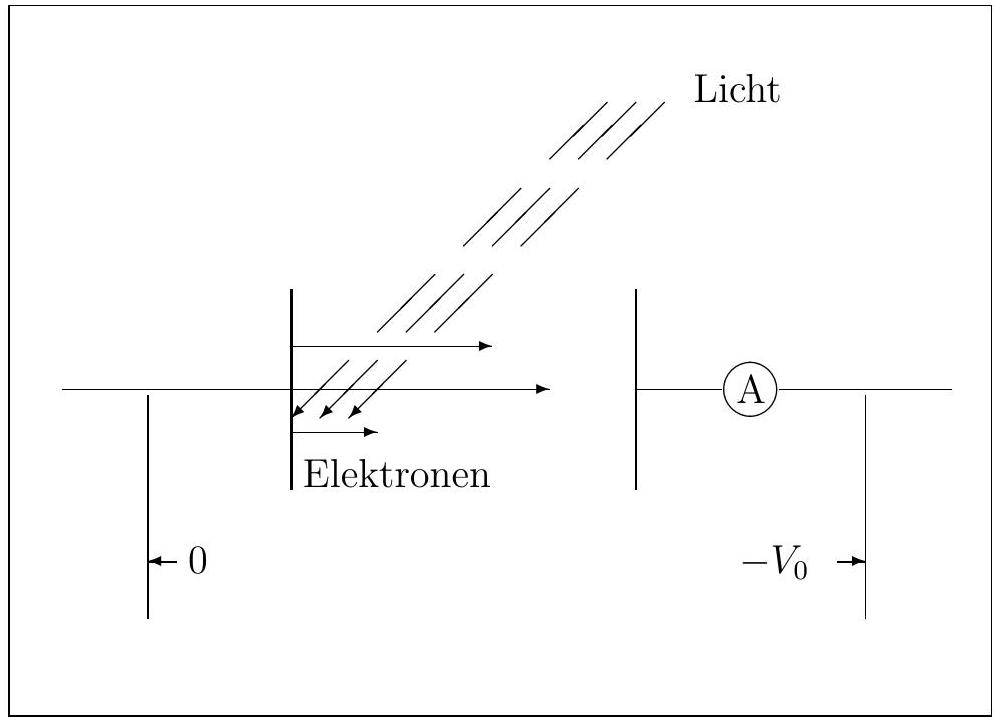
\includegraphics[scale=0.2, center]{2025_05_21_7e716008973ee1b5e8beg-05}

Dabei stellt sich folgendes heraus:

\begin{enumerate}
  \item Energie und Intensität
\end{enumerate}

Die Energie der Elektronen ist unabhängig von der Intensität des Lichtes, aber eine lineare Funktion seiner Frequenz $\omega$.\\
2. Austrittsarbeit

Elektronen werde nur emittiert, falls die Frequenz des Lichtes oberhalb einer bestimmten Schwelle liegt, welche man Austrittsarbeit nennt. Die Grenzfrequenz hängt von der Art des Metalles ab.\\
3. Photostrom

Die Größe des Photostromes durch (A), d.h. die Anzahl der Elektronen, ist proportional zur Intensität des Lichtes.

Dieser Effekt ist ihm Rahmen der klassischen Elektrodynamik nicht zu verstehen, die Energie der austretenden Elektronen sollte proportional zur Intensität $\left(\frac{\epsilon_{0}}{2} \vec{E}_{\omega}^{2}+\frac{1}{2 \mu_{0}} \vec{B}_{\omega}^{2}\right)$ des Lichtes sein.

\section*{Lichtquanten}
Für die Erklärung des Photoeffekts hat Einstein den Nobelpreis erhalten:\\
Das Licht besteht aus Teilchen (Quanten) mit der Energie $\hbar \omega$, falls das Licht die (Kreis-) Frequenz $\omega$ hat. Trifft ein solches Lichtquant auf die Metalloberfläche, so kann\\
es durch Zusammenstoß mit einem Elektron seine Energie auf dieses übertragen. Ist $A$ die "Austrittsarbeit" des Elektrons für das betreffende Metall, so gilt die Energiebilanz:

$$
\frac{1}{2} m_{e} \vec{v}_{e}{ }^{2}+A=\hbar \omega
$$

$m_{e}$ : Masse des Elektrons; $\vec{v}_{e}$ : Geschwindigkeit des Elektrons.\\
A hat die Größenordnung $\mathrm{eV}\left(1 \mathrm{eV}=1.602177 \ldots \cdot 10^{-19} \mathrm{~J}\right)$. Die Intensität des Lichtes ist proportional der Anzahl der Lichtquanten= "Photonen", d.h. je mehr Photonen auf das Metall fallen, desto mehr Elektronen werden herausgelöst.

\section*{Compton Effekt}
Dieser Effekt ist ein unmittelbarer Ausdruck der Teilchennatur des Lichtes: Läßt man Röntgenstrahlen senkrecht auf eine dünne Metallfolie fallen, so werden nach der klassischen Elektrodynamik die Elektronen in der Folie zu Schwingungen angeregt, deren Frequenz die gleiche wie die des Röntgenlichtes ist.\\
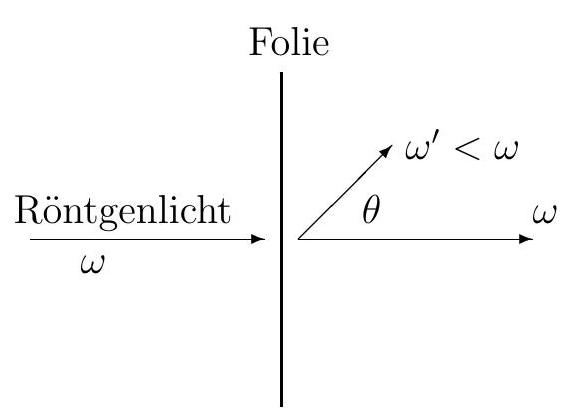
\includegraphics[scale=0.2, center]{2025_05_21_7e716008973ee1b5e8beg-06}

Die Elektronen sollten als schwingende Dipole Röntgenlicht gleicher Frequenz wieder abstrahlen, und zwar unabhängig von der Richtung $\theta$ (s. Skizze). Tatsächlich beobachtet man (Compton) folgendes: Die Frequenz des Lichtes hinter der Folie nimmt mit wachsendem $\theta$ ab!

\section*{Impuls von Photonen}
Wir überlegen uns zunächst, daß aus der speziellen Relativitätstheorie folgt, daß Photonen einen Impuls haben müßen:

$$
\text { relativistisch: } \quad E(\vec{p})=c \sqrt{\vec{p}^{2}+m^{2} c^{2}}
$$

Die Ruhemasse eines Photons (Lichtgeschwindigkeit) verschwindet, also gilt

$$
\text { Photon: } \quad E(\vec{p})=\hbar \omega=\hbar c|\vec{k}|=c|\vec{p}| .
$$

Es folgt dann $|\vec{p}|=\hbar|\vec{k}|$, und da der Ausbreitungsvektor $\vec{k}$ die gleiche Richtung wie $\vec{p}$ hat, ergibt sich

$$
\vec{p}_{P h o t o n} \equiv \vec{p}_{\gamma}=\hbar \vec{k}, \quad|\vec{k}|=2 \pi / \lambda
$$

\section*{Streuung von Photonen an Elektronen}
Man betrachte nun den Compton-Prozeß als elastischen Stoß zwischen Photonen und Elektronen. Die Elektronen befinden sich vor dem Stoß in Ruhe.

Ist nun $\vec{p}_{\gamma}$ der Impuls des Photons ( $\gamma$-Quants) vor dem Stoß mit dem Elektron, $\vec{p}_{\gamma}{ }^{\prime}$ sein Impuls nach dem Stoß und $\overrightarrow{p_{e}{ }^{\prime}}$ der Impuls des Elektrons nach dem Stoß, so lauten Energie- und Impulssatz:

$$
\begin{aligned}
\hbar \omega+m_{e} c^{2} & =\hbar \omega^{\prime}+\left(m_{e}^{2} c^{4}+\left(\vec{p}_{e}^{\prime}\right)^{2} c^{2}\right)^{\frac{1}{2}} \\
\vec{p}_{\gamma} & =\vec{p}_{\gamma}^{\prime}+\vec{p}_{e}^{\prime} \\
m_{e} & : \text { Ruhemasse des Elektrons. }
\end{aligned}
$$

Aus der ersten Gleichung folgt:

$$
\begin{aligned}
m_{e}^{2} c^{4}+\left(\vec{p}_{e}^{\prime}\right)^{2} c^{2} & =\left(\hbar \omega-\hbar \omega^{\prime}+m_{e} c^{2}\right)^{2} \\
& =\left(\hbar \omega-\hbar \omega^{\prime}\right)^{2}+2 m_{e} c^{2}\left(\hbar \omega-\hbar \omega^{\prime}\right)+m_{e}^{2} c^{4} \\
\left(\vec{p}_{e}^{\prime}\right)^{2} & =\frac{\hbar^{2} \omega^{2}}{c^{4}}-\frac{2 \hbar^{2} \omega \omega^{\prime}}{c^{4}}+\frac{\hbar^{2}\left(\omega^{\prime}\right)^{2}}{c^{4}}+\frac{2 m_{e}}{c^{2}}\left(\hbar \omega-\hbar \omega^{\prime}\right)
\end{aligned}
$$

Andererseits ergibt der Impulssatz:

$$
\begin{aligned}
\left(\vec{p}_{e}^{\prime}\right)^{2}=\left(\vec{p}_{\gamma}-\vec{p}_{\gamma}^{\prime}\right)^{2} & =\left(\hbar \vec{k}-\hbar \vec{k}^{\prime}\right)^{2} \\
& =\frac{\hbar^{2} \omega^{2}}{c^{2}}+\frac{\hbar^{2}\left(\omega^{\prime}\right)^{2}}{c^{2}}-2 \frac{\hbar \omega}{c} \frac{\hbar \omega^{\prime}}{c} \cos \theta
\end{aligned}
$$

Einsetzen führt zu

$$
\begin{aligned}
-2 \frac{\hbar \omega}{c} \frac{\hbar \omega^{\prime}}{c} \cos \theta & =-\frac{2 \hbar^{2} \omega \omega^{\prime}}{c^{4}}+\frac{2 m_{e}}{c^{2}}\left(\hbar \omega-\hbar \omega^{\prime}\right) \\
\hbar \omega \omega^{\prime}(1-\cos \theta) & =m_{e} c^{2}\left(\omega-\omega^{\prime}\right)
\end{aligned}
$$

oder, mit $\lambda=2 \pi c / \omega$,

$$
\lambda^{\prime}-\lambda=\frac{2 \pi \hbar}{m_{e} c}(1-\cos \theta)
$$

d.h. die Wellenlänge des abgelenkten Lichtes ist um so größer, je größer der Streuwinkel $\theta$ wird. Das Licht hat also ganz eindeutig Teilcheneigenschaften (Impuls, Energie, etc.).

\section*{Compton-Wellenlänge}
Man kann das "Rückstoß"-Elektron in Koinzidenz mit dem Photon messen (Geiger, Bothe). Die Größe $\lambda_{c}(e)=\hbar / m_{e} c=3.861593 \ldots \cdot 10^{-13} m$ bezeichnet man als Comp-ton-Wellenlänge des Elektrons.

\section*{Materiewellen}
Für Licht gelten die fundamentalen Beziehungen

$$
E=\hbar \omega, \quad \vec{p}=\hbar \vec{k}
$$

zwischen Welleneigenschaften $(\omega, \vec{k})$ auf der einen und den Teilcheneigenschaften $(E, \vec{p})$ auf der anderen Seite.

\section*{Teilchen-Wellen Dualismus}
Dieses motiviert die Hypothese (de Broglie), dass man umgekehrt auch Teilchen Welleneigenschaften zuschreiben können, mit

$$
\begin{aligned}
& \omega=\frac{1}{\hbar} E, \quad \vec{k}=\frac{1}{\hbar} \vec{p} \\
& E=\frac{\vec{p}^{2}}{2 m} \quad \text { oder } \quad E=c\left(\vec{p}^{2}+m^{2} c^{2}\right)^{1 / 2}
\end{aligned}
$$

\section*{de Broglie Wellenlänge}
Wir betrachten Elektron, welche aus der Ruhe auf die Geschwindigkeit $\vec{v}=\vec{p} / m$ gebracht werden, indem man sie eine Potentialdifferenz $U$ durchlaufen läßt. Nach dem Energiesatz gilt

$$
\frac{\vec{p}^{2}}{2 m_{e}}=e U, \quad \frac{1}{2 m_{e}}\left(\frac{2 \pi}{\lambda}\right)^{2} \hbar^{2}=e U
$$

wobei wir $\vec{p}=\hbar \vec{k}$ und $|\vec{k}|=\frac{2 \pi}{\lambda}$ verwendet haben.

$$
\begin{aligned}
\lambda_{e} & =\frac{2 \pi \hbar}{\left(2 m_{e} e U\right)^{\frac{1}{2}}} \\
& \approx\left(\frac{150}{U}\right)^{\frac{1}{2}} \text{\AA}, \quad U \text { in Volt }
\end{aligned}
$$

Die 'de Broglie'-Wellenlänge $\lambda_{e}$ der Elektronen ist also eine Funktion der durchlaufenen Spannung $U$. Bei $U=10^{2}, 10^{3}$ Volt, liegt $\lambda_{e}$ in der Größenordnung von Röntgenstrahlen. Experimente mit Elektronenstrahlen (analog zu den Röntgenspektrometern mit Hilfe von Kristallen als Beugungsgittern) haben ergeben, daß man Elektronen (und ebenso anderen atomaren Teilchen) Welleneigenschaften zuschreiben muß: man hat z.B. Interferenzen, Beugungserscheinungen etc. beobachtet. Da $\lambda \sim(1 / m)^{1 / 2}$, so spielt der Wellenaspekt bei makroskopischen Massen keine Rolle.

\section*{Bohr'sche Atommodell}
Streuversuche mit $\alpha$ - Teilchen und Atomen (Geiger, Marsden u.a.) hatten folgendes Atommodell (Rutherford) nahegelegt:

Die Atome bestehen aus einem nahezu punktförmigen positiven Kern (Radien $\leq 10^{-15} \mathrm{~m}$ ), um den die Elektronen in relativ weitem Abstand (Radius ca. $10^{-10} \mathrm{~m}$ ) "kreisen".

\section*{Atome sind klassisch instabil}
Das klassische AtomeModell kann die Streuexperimente gut erklären (Rutherford'sche Streuformel), führte aber zu prinzipiellen Schwierigkeiten bei den Spektren: Beschleunigte Ladungen strahlen nach der Elektrodynamik elektromagnetische Strahlung ab, deren Intensität proportional zum Quadrat der Beschleunigung ist. Die "kreisenden" Elektronen müßten also ständig strahlen und in ca. $10^{-10}$ sek in den Kern "fallen"; d.h. die Atome wären demnach instabil.

Einen phänomenologischen Ausweg aus dieser Schwierigkeit fand Bohr für wasserstoffartige Atome mit zwei Postulaten.

\section*{Interferierende Materiewellen}
Wir nehmen an, daß sich die Elektronen als selbstinterferierende Materiewellen auf einer Kreisbahn mit dem Radius $r_{n}$ um den Kern bewegt. Die Winkelabhängigkeit der Wellenfunktion des Elektrons ist dann

$$
\sim \mathrm{e}^{i k\left(r_{n} \varphi\right)},
$$

wobei $k=2 \pi / \lambda$ der (noch zu bestimmende) Wellenvektor des Elektron ist. Die Wellenfunktion muss als Funktion des Winkels $\varphi$ eindeutig sein, also

$$
k r_{n} 2 \pi=n 2 \pi, \quad r_{n}=\frac{n}{k}
$$

Für eine feste Quantenzahl $n$ ist der Wellenvektor $k$ dadurch bestimmt, dass durch ihn die Gesamtenergie des umlaufenden Elektrons,

$$
E=\frac{p^{2}}{2 m_{e}}-\frac{Z e^{2}}{4 \pi \epsilon_{0} r_{n}}=\frac{\hbar^{2} k^{2}}{2 m_{e}}-\frac{Z e^{2} k}{4 \pi \epsilon_{0} n}
$$

minimal wird (das entspricht einem Gleichgewicht der mechanischen Kräfte), $Z$ ist dabei die Kernladungszahl:

$$
\frac{\partial E(k)}{\partial k}=\frac{\hbar^{2} k}{m_{e}}-\frac{Z e^{2}}{4 \pi \epsilon_{0} n}=0, \quad k=\frac{m_{e}}{\hbar^{2}} \frac{Z e^{2}}{4 \pi \epsilon_{0} n} .
$$

Setzen wir dieses Ergebnis in $E(k)$ ein, so erhalten wir:

$$
\begin{aligned}
r_{n} & =\frac{4 \pi \varepsilon_{0} n^{2} \hbar^{2}}{Z e^{2} m_{e}} \\
E_{n} & =-\frac{1}{2} m_{e} c^{2} \frac{(\alpha Z)^{2}}{n^{2}}, \quad \alpha=\frac{e^{2}}{4 \pi \varepsilon_{0} \hbar c} .
\end{aligned}
$$

Die vom Maßsystem unabhängige dimensionslose Sommerfeld'sche Feinstrukturkonstante $\alpha$ hat den Zahlenwert $1 /(137.035 \ldots)$.

\section*{Spektren}
Auf den Bahnen $r_{n}$ strahlt das Elektron keine Energie ab. Strahlung findet dagegen statt, falls das Elektron von einem Niveau $E_{n_{2}}$ zu einem Niveau $E_{n_{1}}$ "springt", und zwar wird dabei Licht mit der Frequenz $\omega=\left(E_{n_{2}}-E_{n_{1}}\right) / \hbar$ abgestrahlt.

Diese Annahme ergibt unmittelbar die Balmer'sche Formel für die Spektrallinien des Wasserstoff - Atoms:

$$
\omega_{1,2}=\frac{1}{\hbar} \frac{1}{2} m_{e} c^{2} \alpha^{2} Z^{2}\left(\frac{1}{n_{1}^{2}}-\frac{1}{n_{2}^{2}}\right)
$$

Die Postulate 1 und 2 sind nicht aus der Mechanik und Elektrodynamik begründbar. Erst die Existenz des Wirkungsquantums $\hbar$ macht die Stabilität der Atome möglich.\\
Man bezeichnet mit $a_{0} \equiv r_{1}(Z=1)$ den Bohr'schen Radius:

$$
a_{0}=\frac{4 \pi \varepsilon_{0} \hbar^{2}}{e^{2} m_{e}}=0.529177 \text{\AA}
$$








\pagebreak



\section{Die Schrödinger - Gleichung}

Die in A2 Quantenphysik diskutierten Phänomene zeigen, daß Wellen Teilcheneigenschaften haben, und umgekehrt. Dabei sind für freie Teilchen, bzw. Wellen, die Größen Energie $E(\vec{p})$ und Impuls $\vec{p}$ auf der Teilchenseite mit den Größen Kreisfrequenz $\omega(\vec{k})$ und Wellenvektor $\vec{k}$ auf der Wellenseite durch die fundamentalen Beziehungen

$$
E=\hbar \omega, \quad \vec{p}=\hbar \vec{k}
$$

verknüpft. Dabei ist

$$
\hbar=1.054572 \ldots \cdot 10^{-34} \mathrm{~J} \mathrm{~s}=6.582 \ldots \cdot 10^{-22} \mathrm{MeV} \mathrm{~s}
$$

das Planck'sche Wirkungsquantum (Energie mal Zeit, mit $\hbar=h /(2 \pi))$.

\begin{itemize}
  \item $E=\hbar \omega$ : dass Licht aus Energiequanten (Photonen) besteht, folgt u.A. aus den Eigenschaften der Hohlraumstrahlung, sowie aus dem photoelektrischen Effekt.
  \item $\vec{p}=\hbar \vec{k}$ : Die Verknüpfung von Impuls mit dem Wellenvektor kann aus dem Compton Effekt abgeleitet werden.
\end{itemize}

Ausgehend von dieser Einsicht läßt sich die Schrödinger-Gleichung ableiten, was wir im Folgenden tun werden.

\subsection*{Wellenpakete}
Wellen werden (wie in der Optik) in der Quantenmechanik mittels komplexer Zahlen beschrieben.

\section*{Ebene Wellen}
Ebene Wellen $\psi_{\mathbf{k}}(\vec{x}, t)$ sind wie in der Elektrodynamik durch

$$
\begin{aligned}
\psi_{\mathbf{k}}(\vec{x}, t) & =A(\vec{k}) e^{-i(\omega(\vec{k}) t-\vec{k} \cdot \vec{x})} \\
A(\vec{k}) & : \text { Amplitude } \\
\omega t-\vec{k} \cdot \vec{x} & : \text { Phase }
\end{aligned}
$$

definiert. Falls $|A|=\left[(\Re e A)^{2}+(\Im m A)^{2}\right]^{\frac{1}{2}} \neq 0$, so ist die Welle überall im Raum vorhanden.

\section*{Wellenpakete}
Räumlich begrenzte Wellenzüge, sog. Wellenpakete, entstehen durch Überlagerung von ebenen Wellen mit verschiedenen $\vec{k}$ und $\omega(\vec{k})$.

\section*{Überlagerung zweier ebenen Wellen}
Als einfaches Beispiel für ein Wellenpaket betrachten wir die Überlagerung zweier ebenen Wellen.

Seien $\psi_{\mathbf{k}_{\mathbf{1}}}(\vec{x}, t)$ und $\psi_{\mathbf{k}_{\mathbf{2}}}(\vec{x}, t)$ zwei ebene Wellen mit nur wenig verschiedenen Wellenvektoren $\vec{k}_{i}$. Wir nehmen an, daß $\vec{k}_{i}=\left(k_{i}, 0,0\right)$, die Ausbreitung also in $x_{1}$-Richtung stattfinde. Die Überlagerung (Superposition) der beiden Wellen ist

$$
\psi_{\bar{k}}(\vec{x}, t)=A_{1} e^{-i\left(\omega_{1} t-k_{1} x\right)}+A_{2} e^{-i\left(\omega_{2} t-k_{2} x\right)}
$$

wobei wir $\vec{x}=\left(x_{1}, x_{2}, x_{3}\right)=(x, y, z)$ verwendet haben. Es sei $A_{1}=A_{2}=A$. Ferner setzen wir:

$$
\begin{array}{cc}
\omega_{1}=\bar{\omega}+\Delta \omega \quad, & \omega_{2}=\bar{\omega}-\Delta \omega \\
k_{1}=\bar{k}+\Delta k & , \quad k_{2}=\bar{k}-\Delta k
\end{array}
$$

und erhalten

$$
\begin{aligned}
\psi_{\bar{k}}(\vec{x}, t) & =A\left[e^{-i[(\bar{\omega}+\Delta \omega) t-(\bar{k}+\Delta k) x]}+e^{-i[(\bar{\omega}-\Delta \omega) t-(\bar{k}-\Delta k) x]}\right] \\
& =A\left[e^{-i(t \Delta \omega-x \Delta k)}+e^{+i(t \Delta \omega-x \Delta k)}\right] \cdot e^{-i(\bar{\omega} t-\bar{k} x)} \\
& =2 A \cos (t \Delta \omega-x \Delta k) e^{-i(\bar{\omega} t-\bar{k} x)}
\end{aligned}
$$

Durch Superposition der ebenen Wellen $\psi_{\mathbf{k}_{\mathbf{1}}}, \psi_{\mathbf{k}_{\mathbf{2}}}$ ensteht ein Wellenzug mit der mittleren Frequenz $\bar{\omega}$, dem Wellenvektor $\bar{k}$ und der "modulierten" Amplitude $\tilde{A}=2 A \cos (t \Delta \omega-$ $x \Delta k$ ). Die neue Amplitude $\tilde{A}$ ist eine Funktion von $\vec{x}$ und $t$. Sie ist maximal für

$$
t \Delta \omega-x \Delta k=n \pi, \quad n=0, \pm 1, \cdots
$$

und verschwindet für

$$
t \Delta \omega-x \Delta k=(2 n+1) \frac{\pi}{2}, \quad n=0, \pm 1 \cdots
$$

\section*{Gruppengeschwindigkeit}
Die "Bewegung" des durch $t \Delta \omega-x \Delta k=0$ gegebenen Maximums von $\tilde{A}$ ist durch

$$
\tilde{x}(t)=\frac{\Delta \omega}{\Delta k} t
$$

charakterisiert. Im Limes $\Delta k \rightarrow 0$ wird daraus

$$
\tilde{x}(t)=\frac{\partial \omega}{\partial k} t,
$$

oder, im 3 - dimensionalen Fall,

$$
\overline{\vec{x}}=\left(\operatorname{grad}_{\mathbf{k}} \omega(\vec{k})\right) t
$$

Das Maximum der superponierten Welle wandert also mit der Geschwindigkeit

$$
\vec{v}_{g}:=\operatorname{grad}_{\mathrm{k}} \omega(\vec{k})
$$

durch den Raum. Man bezeichnet diese Geschwindigkeit als Gruppengeschwindigkeit des Wellenzuges (Wellenpaketes).

Wegen $E=\hbar \omega, \vec{p}=\hbar \vec{k}$ gilt

$$
\vec{v}_{g}=\operatorname{grad}_{\mathbf{p}} E(\vec{p})=\vec{v}
$$

Die Gruppengeschwindigkeit eines Wellenpaketes ist gleich der "mechanischen" Geschwindigkeit der zugeordneten Teilchen.

Man betrachte z.B. $E(\vec{p})=\vec{p}^{2} /(2 m)$. Dies ist ein wichtiger Zusammenhang zwischen Wellen- und Teilcheneigenschaften.

\section*{Phasengeschwindigkeit}
Die Ausbreitung der Wellenphase $\bar{\omega} t-\bar{k} x$ ist durch $\bar{\omega} t-\bar{k} x=$ const. charakterisiert und durch $v_{\text {phase }}=\bar{\omega} / \bar{k}$ gegeben. Man bezeichnet sie mit Phasengeschwindigkeit. Wie wir von den Radiowellen wissen, findet die Übertragung der "Information" via der Modulation der Amplitude statt, die Information breitet sich also mit der Gruppengeschwindigkeit $\vec{v}_{g}$ aus.

\section*{Allgemeines Wellenpaket}
Im allgemeinen enthält ein Wellenzug (Wellenpaket) unendlich viele Frequenzen,

$$
\psi(\vec{x}, t)=\int_{-\infty}^{+\infty} \int_{-\infty}^{+\infty} \int_{-\infty}^{+\infty} d^{3} k g(\vec{k}) e^{-i(\omega(\vec{k}) t-\vec{k} \cdot \vec{x})}
$$

was einer Fourier-Zerlegung mit (komplexen) Fourier-Komponenten $g(\vec{k})$ entspricht. Letzter bestimmen, mit welchem Gewicht einzelne ebenen Wellen $\psi_{\mathbf{k}}(\vec{x}, t)$ an dem Wellenpaket beteiligt sind.

\subsubsection*{Gauß'sche Wellenpakete}
Für eine Motivation der Unschärfe-Relation betrachten wir hier den eindimensionallen Fall.

\section*{Gauß'sches Wellenpaket für den eindimensionalen Fall}
Die Funktion

$$
g(k)=e^{-\alpha\left(k-k_{o}\right)^{2}}, \quad \alpha>0
$$

beschreibt eine Gauß'sche Verteilung, die bei $k=k_{0}$ konzentriert ist. Die Breite $\sigma$ der Verteilung ist durch den Parameter $\alpha=1 /\left(2 \sigma^{2}\right)$ charakterisiert. Das Wellenpaket lautet

$$
\psi(x, t)=\int_{-\infty}^{+\infty} d k e^{-\alpha\left(k-k_{0}\right)^{2}} e^{-i(\omega(k) t-k x)}
$$

Die klasssiche $E=p^{2} /(2 m)$ und die relativistische $E^{2}=c^{2} p^{2}+m^{2} c^{4}$ Energie-Impuls Beziehungen für freie Teilchen führen jeweils zu

$$
\begin{aligned}
\omega & =\frac{1}{\hbar} \frac{1}{2 m}(\hbar k)^{2}=\frac{\hbar}{2 m} k^{2} \\
\omega & =\frac{1}{\hbar} c \sqrt{\left.(\hbar k)^{2}+m^{2} c^{2}\right)}=c\left(k^{2}+\left(\frac{m c}{\hbar}\right)^{2}\right)^{\frac{1}{2}}
\end{aligned}
$$

wobei wir $E=\hbar \omega$ und $p=\hbar k$ verwendet haben. Allgemein ist Entwicklung von $\omega(k)$ um $k=k_{0}$

$$
\omega(k)=\omega\left(k_{0}\right)+\left.\frac{d \omega}{d k}\right|_{k=k_{0}}\left(k-k_{0}\right)+\left.\frac{1}{2} \frac{d^{2} \omega}{d k^{2}}\right|_{k=k_{0}}\left(k-k_{0}\right)^{2}+\cdots
$$

Für das Gauß'sche Wellenpaket ist die Verteilung $\omega(k)$ um $k=k_{0}$ konzentriert, wir können also die Entwicklung nach dem zweiten Glied abbrechen (für $\omega=\frac{\hbar}{2 m} k^{2}$ wäre dies exakt).

$$
\begin{array}{rlrl}
\left.\frac{d \omega}{d k}\right|_{k=k_{0}} & =v_{g} & & \text { (Gruppengeschwindigkeit) } \\
\left.\frac{1}{2} \frac{d^{2} \omega}{d k^{2}}\right|_{k=k_{0}} & \equiv \beta & \left(\rightarrow \frac{\hbar}{2 m} \quad \text { für } \quad \omega=\frac{\hbar}{2 m} k^{2}\right)
\end{array}
$$

Für das Wellenpaket ergibt sich damit

$$
\psi(x, t)=\int_{-\infty}^{+\infty} d k e^{-\alpha\left(k-k_{0}\right)^{2}} e^{-i\left[\omega\left(k_{0}\right) t+v_{g}\left(k-k_{0}\right) t+\beta\left(k-k_{0}\right)^{2} t-k x\right]}
$$

Wir führen die Variablen-Substitution $\tilde{k}=k-k_{0}$ durch:

$$
\psi(x, t)=e^{-i\left(\omega\left(k_{0}\right) t-k_{0} x\right)} \int_{-\infty}^{+\infty} d \tilde{k} e^{-\alpha \tilde{k}^{2}-i \beta t \tilde{k}^{2}} e^{i \tilde{k}\left(x-v_{g} t\right)}
$$

Das Gauss'sche Integral ergibt (Übungen)

$$
\int_{-\infty}^{+\infty} d y e^{-\gamma y^{2}} e^{-i u y}=\sqrt{\frac{\pi}{\gamma}} \exp \left(-\frac{1}{4 \gamma} u^{2}\right)
$$

Diese Formel gilt auch für komplexe $\gamma$, falls $\Re e \gamma>0$, so daß wir insgesamt zu folgendem Resultat gelangen:

$$
\psi(x, t)=\left(\frac{\pi}{\alpha+i \beta t}\right)^{\frac{1}{2}} e^{-\frac{1}{4(\alpha+i \beta t)}\left(x-v_{g} t\right)^{2}} e^{-i\left(\omega\left(k_{0}\right) t-k_{0} x\right)}
$$

Das Wellenpaket $\psi(x, t)$ ist eine Welle mit der Phase $\omega\left(k_{0}\right) t-k_{0} x$ und der ortsabhängigen Amplitude

$$
\begin{aligned}
A_{G}(x, t) & =\left(\frac{\pi}{\alpha+i \beta t}\right)^{\frac{1}{2}} e^{-\frac{1}{4(\alpha+i \beta t)}\left(x-v_{g} t\right)^{2}} \\
\left|A_{G}(x, t)\right|^{2}=A_{G} A_{G}^{*} & =\left(\frac{\pi^{2}}{\alpha^{2}+\beta^{2} t^{2}}\right)^{\frac{1}{2}} e^{-\frac{\alpha\left(x-v_{g} t\right)^{2}}{2\left(\alpha^{2}+\beta^{2} t^{2}\right)}}
\end{aligned}
$$

Die Intensität $|\psi(x, t)|^{2}=\left|A_{G}\right|^{2}$ ist also wieder eine Gauß'sche Verteilung. Mit $\sigma^{2}=$ $\left(\alpha^{2}+\beta^{2} t^{2}\right)$ wächst die Varianz $\sigma$ mit der Zeit.

\section*{Gruppengeschwindingkeit}
Bei festem $t$ ist $|\psi(x, t)|^{2}$ maximal, falls $x=v_{g} t$, d.h. dort, wo sich nach der klassischen Mechanik $(x(t)=v t)$ das Teilchen befinden sollte. Das Maximum wandert mit der Geschwindigkeit $v_{g}$.

\section*{Unschärfe-Relation}
Für $t=0$ ist

$$
|\psi(x, 0)|^{2}=\frac{\pi}{\alpha} e^{-\frac{x^{2}}{2 \alpha}} \equiv \frac{\pi}{\alpha} e^{-\frac{x^{2}}{2 \sigma_{x}^{2}}}
$$

was wir mit

$$
|g(k)|^{2}=e^{-2 \alpha\left(k-k_{0}\right)^{2}} \equiv e^{-\frac{\left(k-k_{0}\right)^{2}}{2 \sigma_{k}^{2}}}
$$

in Verbindung setzten können. Wir definieren

$$
\begin{aligned}
& \delta x(0)=\sqrt{2 \alpha}: \begin{array}{l}
\text { Breite des Wellenpaketes im Ortsraum zur } \\
\text { Zeit } \mathrm{t}=0
\end{array} \\
& \delta k:=1 / \sqrt{2 \alpha}: \begin{array}{l}
\text { Breite des Gauß'schen Wellenpaketes } \\
\text { im } k \text {-Raum }
\end{array}
\end{aligned}
$$

denn, z.B. falls $k-k_{0}=\delta k$, so ist $|g(k)|^{2}$ auf den $e$ - ten Teil abgefallen. Zwischen $\delta x(0)$ und $\delta k$ gilt die Beziehung

$$
\delta k \delta x(0)=1
$$

Je schmaler also ein Wellenpaket im $k$ - Raum ist (d.h. je schmaler die Spektrallinie ist), um so breiter ist das Wellenpaket im Ortsraum und umgekehrt. ${ }^{1}$ Mit $p=\hbar k$ folgt schlussendlich

$$
\delta p \delta x(0)=\hbar
$$

Je genauer man also den Impuls eines Teilchens kennt ("Unschärfe" $\delta p$ ), desto weniger genau kann man seinen Ort $x$ angeben ("Unschärfe" $\delta x$ ). Das Produkt der Unschärfen ist durch $\hbar$ gegeben was die Heisenberg'sche Unschärferelation definiert. Mehr hierzu später!

\section*{Born'sche Interpretation}
Die Unschärferelation gilt - wie wir sehen werden - für beliebige Wellenpakete. Sie bedeutet, daß die Wellenfunktion nicht die Materieverteilung eines Teilchens beschreiben kann, denn erfahrungsgemäß zerfließen Elektronen, Protonen und Atome nicht.

Nach Born ist $|\psi(x, t)|^{2}$ vielmehr als Wahrscheinlichkeitsdichte zu interpretieren, wie wir weiter unten noch ausführlicher diskutieren werden.

\subsection*{Schrödinger - Gleichung}
\subsubsection*{Herleitung für freie Teilchen}
Mit $E=\hbar \omega$ und $\vec{p}=\hbar \vec{k}$ nimmt die ebene Welle $\psi_{\mathbf{k}}(\vec{x}, t)=A e^{-i(\omega t-\vec{k} \cdot \vec{x})}$ die Form

$$
\psi_{\mathbf{p}}(\vec{x}, t)=A e^{-\frac{i}{\hbar}(E t-\vec{p} \cdot \vec{x})}
$$

an. Für ein nichtrelativistisches Teilchen hat man $E=\frac{1}{2 m} \vec{p}^{2}$. Mit

$$
\partial_{t} \psi_{\mathbf{p}}(\vec{x}, t)=-\frac{i}{\hbar} E \psi_{\mathbf{p}}(\vec{x}, t)
$$

und

$$
\frac{\partial}{\partial x_{j}} \psi_{\mathbf{p}}(\vec{x}, t) \equiv \partial_{j} \psi_{\mathbf{p}}(\vec{x}, t)=\frac{i}{\hbar} p_{j} \psi_{\mathbf{p}}(\vec{x}, t)
$$

folgt

$$
\begin{aligned}
\Delta \psi_{\mathbf{p}}(\vec{x}, t) \equiv\left(\partial_{1}^{2}+\partial_{2}^{2}+\partial_{3}^{2}\right) \psi_{\mathbf{p}}(\vec{x}, t) & =-\frac{1}{\hbar^{2}} \vec{p}^{2} \psi_{\mathbf{p}}(\vec{x}, t) \\
& =-\frac{2 m}{\hbar^{2}} E \psi_{\mathbf{p}}(\vec{x}, t)
\end{aligned}
$$

Also genügt $\psi_{\mathbf{p}}(\vec{x}, t)$ der (partiellen) Differentialgleichung

$$
i \hbar \partial_{t} \psi_{\mathbf{p}}(\vec{x}, t)=-\frac{\hbar^{2}}{2 m_{e}} \Delta \psi_{\mathbf{p}}(\vec{x}, t)
$$

Analog gilt für das Integral

$$
\psi(\vec{x}, t)=(2 \pi \hbar)^{-\frac{3}{2}} \int_{-\infty}^{+\infty} \widetilde{\psi}(\vec{p}) e^{-\frac{i}{\hbar}\left(\frac{\vec{p}^{2}}{2 m} t-\vec{p} \cdot \vec{x}\right)} d^{3} p
$$

die Schrödinger-Gleichung.


$$
i \hbar \partial_{t} \psi(\vec{x}, t)=-\frac{\hbar^{2}}{2 m_{e}} \Delta \psi(\vec{x}, t)
$$

für freie Teilchen.

\section*{Superpositionsprinzip}
Die Schrödinger-Gleichung ist eine lineare partielle Differentialgleichung in den Zeit- und Orts-koordinaten. Die Linearität trägt dem für die Quantentheorie fundamentalen Superpositionsprinzip Rechnung:

Beschreiben $\psi_{1}$ und $\psi_{2}$ zwei quantentheoretisch mögliche physikalische Zustände, so beschreibt auch die lineare Superpostion

$$
c_{1} \psi_{1}+c_{2} \psi_{2}, \quad c_{i} \in \mathcal{C}
$$

einen möglichen physikalischen Zustand.
\section*{Korrespondenzprinzip}
Man erhält die freie Schrödinger-Gleichung formal, indem man in der Beziehung $E=\frac{1}{2 m} \vec{p}^{2}$ folgende Zuordnungen macht:

$$
E \rightarrow i \hbar \partial_{t}, \quad p_{j} \rightarrow \mathbf{P}_{j}:=\frac{\hbar}{i} \partial_{j}
$$

sowie

$$
\frac{1}{2 m} \vec{p}^{2} \quad \rightarrow \quad \frac{1}{2 m} \overrightarrow{\mathbf{P}}^{2}=-\frac{\hbar^{2}}{2 m_{e}} \Delta \equiv \mathbf{H}_{0}
$$

Die Differential-Operatoren $i \hbar \partial_{t}$ und $\mathbf{H}_{0}$ sind auf die Wellenfunktion $\psi(\vec{x}, t)$ anzuwenden. Aus $E=\frac{1}{2 m} \vec{p}^{2}$ folgt dann die freie Schrödinger-Gleichung:

$$
i \hbar \partial_{t} \psi(\vec{x}, t)=\mathbf{H}_{0} \psi(\vec{x}, t)=-\frac{\hbar^{2}}{2 m_{e}} \Delta \psi(\vec{x}, t)
$$

\subsubsection*{Teilchen in äußerem Potential}
Ein klassisches Teilchen, das sich in einem Potential $V(\vec{x})$ (unabhängig von $t$ und $\vec{p}$) befindet, besitzt die Gesamtenergie $E=\frac{1}{2 m} \vec{p}^{2}+V(\vec{x})$. Die Verallgemeinerung des obigen freien Falles ist dann

$$
E \rightarrow \mathbf{H}:=\mathbf{H}_{0}+V(\vec{x})=-\frac{\hbar^{2}}{2 m_{e}} \Delta+V(\vec{x})
$$

mit dem Konventionsfaktor $(2 \pi \hbar)^{-3/2}$\footnote{Dieser Faktor ist Konvention.} erhält man schließlich die zugehörige Schrödinger-Gleichung:

$$
i \hbar \partial_{t} \psi(\vec{x}, t)=\mathbf{H} \psi(\vec{x}, t)=-\frac{\hbar^{2}}{2 m_{e}} \Delta \psi(\vec{x}, t)+V(\vec{x}) \psi(\vec{x}, t)
$$

Die Schrödinger-Gleichung mit Potential ist eine lineare Differentialgleichung, also gilt auch hier das Superpositionsprinzip. Umgekehrt folgt die Linearität der SchrödingerGleichung für ein Teilchen mit Wechselwirkung aus der Forderung nach Gültigkeit des Superpositionsprinzipes für Wellenfunktionen.

Man beachte, daß das Superpositionsprinzip in der Mechanik i.allg. nicht gilt, da die (Hamilton'schen) Bewegungsgleichungen i.allg. nicht linear sind.

\section*{Plausibilitätsbetrachtung}
Die Schrödinger-Gleichung

$$
i \hbar \partial_{t} \psi(\vec{x}, t)=\left(-\frac{\hbar^{2}}{2 m_{e}} \Delta+V(\vec{x})\right) \psi(\vec{x}, t)
$$

für ein Teilchen in einem klassischen äußeren Potential $V(\vec{x})$ kann man sich folgendermaßen plausibel machen:\\
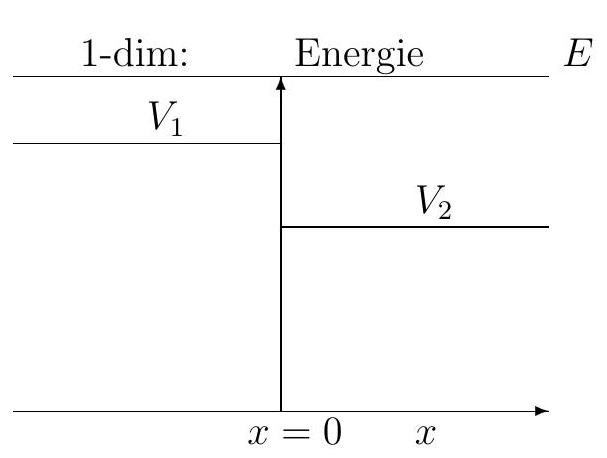
\includegraphics[scale=0.2, center]{2025_05_21_11b1754c718f6fcf84f8g-08}

Teilchen der Energie $E$ befinden sich für $x<0$ in einem Potential $V_{1}>0$ und für $x>0$ in $V_{2} \geq 0, V_{1}>V_{2}$.\\
Z.B.\\
$x<0$ : Elektronen in einem Leiter $x>0$ : im leeren Raum

In beiden Fällen, $j=1,2$, sind den Teilchenstrahlen ebene Wellen zugeordnet:

$$
\begin{aligned}
\psi_{j} & =A_{j} e^{-\frac{i}{\hbar}\left(E t-p_{j} x\right)}, \quad p_{j}=\left[2 m\left(E-V_{j}\right)\right]^{\frac{1}{2}} \\
E & =\frac{1}{2 m} p_{1}^{2}+V_{1}=\frac{1}{2 m} p_{2}^{2}+V_{2}
\end{aligned}
$$

Für $x<0$ bzw. $x>0$ gelten jeweils die Gleichungen

$$
\begin{aligned}
i \hbar \partial_{t} \psi_{1}(x, t) & =-\frac{\hbar^{2}}{2 m} \frac{d^{2}}{d x^{2}} \psi_{1}(x, t)+V_{1} \psi_{1}(x, t) \\
i \hbar \partial_{t} \psi_{2}(x, t) & =-\frac{\hbar^{2}}{2 m} \frac{d^{2}}{d x^{2}} \psi_{2}(x, t)+V_{2} \psi_{2}(x, t)
\end{aligned}
$$

Hat man nun $n$ verschiedene Gebiete mit $V_{\nu}=$ const. $\nu=1, \ldots n$, mit $V_{\nu_{1}} \neq V_{\nu_{2}}$, so erhält man für jedes $\nu$ eine entsprechende Gleichung wie oben. Eine naheliegende (aber\\
nicht zwingende) Verallgemeinerung für kontinuierliche $V(x)$ ist dann:

$$
i \hbar \partial_{t} \psi(x, t)=\left(-\frac{\hbar^{2}}{2 m} \frac{d^{2}}{d x^{2}}+V(\vec{x})\right) \psi(x, t)
$$

Die eigentliche Bestätigung der Schrödinger - Gleichung erhält man durch Vergleich mit experimentellen Resultaten.

\subsubsection*{Operatoren}
Operatoren sind nichts anderes als Vorschriften, wie Elemente einer vorgegebenen Menge bestimmte Elemente einer anderen Menge (die gleich der ursprünglichen sein kann) zugeordnet werden. Ein anderer Name für derartige Vorschriften ist Abbildung.

\section*{Matrizen}
Es sei $\left(\mathbf{e}_{\mathbf{1}}, \mathbf{e}_{\mathbf{2}}\right)$ eine feste Basis im $\mathbb{R}^{2}$. Man hat dann

$$
\vec{x}=x_{1} \mathbf{e}_{\mathbf{1}}+x_{2} \mathbf{e}_{\mathbf{2}} \quad \leftrightarrow \quad\binom{x_{1}}{x_{2}}=\mathbf{x}
$$

Jede Matrix

$$
\mathbf{A}=\left(\begin{array}{ll}
a_{11} & a_{12} \\
a_{21} & a_{22}
\end{array}\right)
$$

definiert eindeutig eine Abbildung $\mathbb{R}^{2} \rightarrow \mathbb{R}^{2}$ durch, die Vorschrift

$$
\mathbf{x} \quad \rightarrow \quad \mathbf{x}_{\mathbf{A}}=\mathbf{A} \cdot \mathbf{x} \quad \text { für alle } \mathbf{x} \in \mathbb{R}^{2} .
$$

Hier ist A ein Matrix - Operator.

\section*{Beispiele für Operatoren}
$\overline{\text { Es sei }} \mathcal{F}:=\left\{f_{1}(x), \cdots, f_{n}(x), x \in \mathbb{R}\right\}$ eine Menge von komplexwertigen Funktionen auf der reellen Achse, die bestimmte Eigenschaften haben. Z.B. seien die $f_{\nu}(x)$ quadratintegrierbar:

$$
\int_{\mathbb{R}} d x\left|f_{\nu}(x)\right|^{2}<\infty
$$

\begin{itemize}
  \item Multiplikations-Operator
\end{itemize}

Die Vorschrift

$$
f_{\nu}(x) \rightarrow x^{2} f_{\nu}(x)
$$

definiert den Multiplikations - Operator $x^{2}$. Man beachte, daß häufig $x^{2} f_{\nu}(x) \notin \mathcal{F}$ : so braucht z.B. $x^{2} f_{\nu}(x)$ nicht mehr quadratintegrabel zu sein!

\begin{itemize}
  \item Differential-Operator Die Vorschrift
\end{itemize}

$$
f_{\nu}(x) \rightarrow \frac{d}{d x} f_{\nu}(x)
$$

definiert den Differential-Operator $\frac{d}{d x}$, falls $f_{\nu} \in C^{1}$ (d.h. die Menge der 1-mal stetig differenzierbaren Funktionen). Auch hier stimmt die Bildmenge nicht notwendigerweise mit der Urbildmenge $C^{1}$ überein!

\begin{itemize}
  \item Komplexe-Konjugation
\end{itemize}

Die Vorschrift

$$
f_{\nu}(x) \rightarrow f_{\nu}^{*}(x)
$$

definiert den Operator der Komplexe Konjugation K.

\section*{Anmerkungen}
\begin{enumerate}
  \item Definitions- und Wertebereich
\end{enumerate}

Diese Beispiele zeigen, daß es bei einem Operator wesentlich ist, die zugehörige

\begin{itemize}
  \item Urbild-Menge = Definitionsbereich
  \item Bild-Menge = Wertebereich\\
anzugeben.
\end{itemize}

\begin{enumerate}
  \setcounter{enumi}{1}
  \item Lineare Operatoren\\
$\overline{\text { Der Matrix-Operator } \mathbf{A}}$ ist ein linearer Operator. Mit
\end{enumerate}

$$
\mathbf{x}^{(1)}, \mathbf{x}^{(2)} \in \mathbb{R}^{2}, \quad \lambda_{1}, \lambda_{2} \in \mathbb{R}, \quad \lambda_{1} \mathbf{x}^{(1)}+\lambda_{2} \mathbf{x}^{(2)} \in \mathbb{R}^{2}
$$

gilt

$$
\mathbf{A} \cdot\left(\lambda_{1} \mathbf{x}^{(1)}+\lambda_{2} \mathbf{x}^{(2)}\right)=\lambda_{1}\left(\mathbf{A} \cdot \mathbf{x}^{(1)}\right)+\lambda_{2}\left(\mathbf{A} \cdot \mathbf{x}^{(2)}\right)
$$

Der Differential-Operator ist gleichfalls linear. Mit

$$
f_{1}(x), f_{2}(x) \in C^{1}, \quad \lambda_{1}, \lambda_{2} \in \mathbb{C}
$$

gilt

$$
\frac{d}{d x}\left(\lambda_{1} f_{1}(x)+\lambda_{2} f_{2}(x)\right)=\lambda_{1} \frac{d}{d x} f_{1}(x)+\lambda_{2} \frac{d}{d x} f_{2}(x)
$$

\begin{enumerate}
  \setcounter{enumi}{2}
  \item Antilineare Operatoren
\end{enumerate}

Andererseis gilt für die komplexe Konjugation $\mathbf{K}$ :

$$
\mathbf{K}\left(\lambda_{1} f_{1}(x)+\lambda_{2} f_{2}(x)\right)=\lambda_{1}^{*} \mathbf{K} f_{1}(x)+\lambda_{2}^{*} \mathbf{K} f_{2}(x),
$$

d.h. $\mathbf{K}$ ist nicht linear. Man nent $\mathbf{K}$ antilinear.\\
4. Vertauschungsrelationen\\
$\overline{\text { Operatoren vertauschen }}$ im allgemeinen nicht miteinander. Seien z.B. $\mathbf{A}_{1}$ und $\mathbf{A}_{2}$ zwei Matrizen, so gilt i.a.

$$
\mathbf{A}_{1} \cdot \mathbf{A}_{2} \neq \mathbf{A}_{2} \cdot \mathbf{A}_{1}, \quad\left[\mathbf{A}_{1}, \mathbf{A}_{2}\right] \equiv \mathbf{A}_{1} \cdot \mathbf{A}_{2}-\mathbf{A}_{2} \cdot \mathbf{A}_{1} \neq 0
$$

Man nennt $\left[\mathbf{A}_{1}, \mathbf{A}_{2}\right]$ den Kommutator von $\mathbf{A}_{1}$ mit $\mathbf{A}_{2}$. Ferner hat man

$$
\frac{d}{d x}(x f(x))=f(x)+x\left(\frac{d}{d x} f(x)\right), \quad \frac{d}{d x}(x f(x))-x\left(\frac{d}{d x} f(x)\right)=f(x)
$$

Das bedeutet

$$
\frac{d}{d x} x-x \frac{d}{d x}=\left[\frac{d}{d x}, x\right]=\mathbf{1}
$$

wobei 1 der Idenditätsoperator (die Einheitsmatrix) ist.\\
5. Skalarprodukt

In jedem komplex-wertigen Vektorraum mit

$$
\mathbf{x}, \mathbf{y} \in \mathcal{C}^{N}, \quad \mathbf{x}=\left(x_{1}, \ldots, x_{N}\right), \quad \mathbf{y}=\left(y_{1}, \ldots, y_{N}\right)
$$

läßt sich das Skalarprodukt

$$
(\mathbf{x}, \mathbf{y}) \equiv \sum_{i} x_{i}^{*} y_{i}, \quad(\mathbf{x}, \mathbf{x})=\sum_{i} x_{i}^{*} x_{i} \equiv|\mathbf{x}|^{2}
$$

definieren. Man bezeichnet $|\mathbf{x}|$ als die Norm des Vektors $\mathbf{x}$. Sei $A$ eine $N \times N$ matrix, dann gilt

$$
(\mathbf{x}, A \mathbf{y})=\sum_{i} x_{i}^{*} A_{i j} y_{i}
$$

\subsubsection*{Das Korrespondenzprinzip}
\section*{Ortsoperators}
Der lineare Multiplikations-Operatore

$$
\mathbf{Q}_{j}: \quad \mathbf{Q}_{j} \psi=x_{j} \psi, \quad j=1,2,3
$$

wird Ortsoperator genannt.

\section*{Impulsoperator}
Der linearen Differential-Operator

$$
\mathbf{P}_{j}: \quad \mathbf{P}_{j} \psi=\frac{\hbar}{i} \partial_{j} \psi, \quad j=1,2,3
$$

wird Impulsoperator genannt.

\section*{Linearität des Schrödinger-Operators}
Der Schrödinger-Operator

$$
\mathbf{H}=-\frac{\hbar^{2}}{2 m_{e}} \Delta+V(\vec{x})
$$

ist ein linearer Operator im Raum der Wellenfunktionen $\psi(\vec{x}, t)$. Er ist mit

$$
\mathbf{H}=\mathbf{H}(\overrightarrow{\mathbf{P}}, \overrightarrow{\mathbf{Q}})=\frac{1}{2 m} \overrightarrow{\mathbf{P}}^{2}+V(\overrightarrow{\mathbf{Q}})
$$

eine Funktion des Orts- und des Impulsoperators.

\section*{Vertauschungs-Relationen}
Die Operatoren $\mathbf{P}_{j}$ und $\mathbf{Q}_{k}$ genügen den Vertauschungs-Relationen:

$$
\begin{aligned}
\mathbf{P}_{j} \mathbf{Q}_{k}-\mathbf{Q}_{k} \mathbf{P}_{j} & =\frac{\hbar}{i} \delta_{j k} \\
\mathbf{P}_{j}\left(\mathbf{Q}_{k} \psi\right)-\mathbf{Q}_{k}\left(\mathbf{P}_{j} \psi\right) & =\left\{\begin{array}{rll}
\frac{\hbar}{i} \psi & \text { für } & j=k \\
0 & \text { für } & j \neq k
\end{array}\right.
\end{aligned}
$$

Weitere Eigenschaften der Operatoren $\mathbf{H}, \overrightarrow{\mathbf{P}}, \overrightarrow{\mathbf{Q}}$ etc. werden später diskutiert.

\section*{Hamilton-Operator}
Der Schrödinger Operator ist eine Funktion von Impuls und Ort, genau wie die HamiltonFunktion der klassischen Mechanik. Daher wird er auch Hamilton-Operator genannt.

\section*{Korrespondenzprinzip}
Der Übergang von der Hamilton-Mechanik zur Quantenmechanik bezeichnet man auch als Quantisierung. Dabei geht man von den "kanonisch konjungierten" Variablen $q_{i}$ und $p_{i}$ (Ort und Impuls) der Hamilton-Mechanik aus. Es gelten die folgende Äquivalenzen:

\section*{Mechanik}
Phasenraum

$$
A\left(q_{i}, p_{i}\right)
$$

\section*{Quantenmechanik}
Hilbertraum\\
Operator $\hat{A}$

Hamiltonfunktion $H$ Hamiltonoperator $\hat{H}$

$$
\begin{aligned}
q_{i}, p_{i} & \text { Operatoren } \hat{q}_{i}, \hat{p}_{i} \\
\{A, B\} & \text { Kommutator }[\hat{A}, \hat{B}]=\hat{A} \hat{B}-\hat{B} \hat{A} \\
\left\{q_{i}, p_{j}\right\}=0 & {\left[\hat{q}_{i}, \hat{p}_{j}\right]=i \hbar \delta_{i j} }
\end{aligned}
$$

\begin{enumerate}
  \setcounter{enumi}{7}
  \item $\quad \frac{d A}{d t}=\frac{\partial A}{\partial t}+\{A, H\} \quad i \hbar \frac{d}{d t} \hat{A}=i \hbar \frac{\partial \hat{A}}{\partial t}+[\hat{A}, \hat{H}]$
\end{enumerate}

Dabei bezeichnet

$$
\{\varphi, \psi\}=\sum_{i}\left(\frac{\partial \varphi}{\partial q_{i}} \frac{\partial \psi}{\partial p_{i}}-\frac{\partial \varphi}{\partial p_{i}} \frac{\partial \psi}{\partial q_{i}}\right)
$$

die Poisson-Klammer $\{\varphi, \psi\}$. Die obrige Tabelle beschreibt das sogenannte "Korrespondenzprinzip". Insbesondere sieht man aus Punkt 7. und 8., dass der klassische Grenzfall $\hbar \rightarrow 0$ erfüllt ist.

\subsection*{Zur Interpretation der Wellenfunktion}
Es sei klassisch $E=\frac{1}{2} \vec{p}^{2}+V_{0}$, mit $V_{0}=$ const. Da die Normierung der Energie (d.h. $V_{0}$ ) willkürlich ist, kann die Frequenz $\omega=E / \hbar$ selbst keine physikalische Bedeutung haben, wohl aber Differenzen, wie $\omega_{12}=\left(E_{2}-E_{1}\right) / \hbar$.

\subsubsection*{Wahrscheinlichkeitsdichte}
Die Wellenfunkion $\psi(\vec{x}, t)$ ist folgendermaßen zu verstehen

Die Größe

$$
w(\vec{x}, t)=|\psi(\vec{x}, t)|^{2}=\psi^{*}(\vec{x}, t) \psi(\vec{x}, t)
$$

ist eine Wahrscheinlichkeitsdichte. Die Wahrscheinlichkeit $w(G, t)$ ein Teilchen zur Zeit $t$ im Gebiet $G \subset \mathbb{R}^{3}$ zu finden, ist entsprechend durch

$$
w(G, t)=\int_{G} d^{3} x w(\vec{x}, t)
$$

gegeben.

\section*{Normierung}
Da das Teilchen irgendwo sein muß, muss die Wellenfunktion normiert sein:

$$
w\left(\mathbb{R}^{3}, t\right)=1
$$

Dies ist eine zusätzliche Bedingung an die Lösungen der Schrödinger-Gleichung: Es sind nur quadrat-integrable Lösungen zugelassen,

$$
\int_{\mathbb{R}^{3}} d^{3} x|\psi|^{2}<\infty
$$

Diese Normierung läßt sich i.A. durch eine einfache Reskalierung der Wellenfunktion erreichen. Falls

$$
\int_{\mathbb{R}^{3}} d^{3} x|\psi|^{2}=N^{2}<\infty
$$

so ist mit $\psi(\vec{x}, t)$ auch

$$
\frac{1}{|N|} \psi(\vec{x}, t)
$$

eine Lösung der Schrödinger - Gleichung, da diese linear ist. Also läßt sich durch Umnormierung immer $\int_{\mathbb{R}^{3}} d^{3} x|\psi|^{2}=1$ erreichen.

\section*{Normierung von Gauß'schen Wellenpakten}
In Abschnitt 1.1.1 haben wir eindimensionale Gauß'sche Wellenpakte behandelt. In drei Dimensionen gilt analog:

$$
\psi_{G}(\vec{x}, t) \approx A_{G}(\vec{x}, t) e^{-i(\omega t-\vec{x} \cdot \vec{k})}, \quad\left|A_{G}(\vec{x}, t=0)\right|^{2}=\left(\frac{\pi}{\alpha}\right)^{3} e^{-\vec{x}^{2} /(2 \alpha)}
$$

wenn wir uns für die Normierung zunächst auf $t=0$ beschränken. Aus $\int d y e^{-y^{2} /(2 \alpha)}=$ $\sqrt{2 \pi \alpha}$ folgt

$$
\int d^{3} x\left|A_{G}(\vec{x}, t=0)\right|^{2}=\left(\frac{\pi}{\alpha}\right)^{3}(2 \pi \alpha)^{\frac{3}{2}}=N^{2}
$$

für die Norm. Demnach erhält man

$$
\begin{aligned}
\psi_{G}(\vec{x}, t=0) & =(2 \pi \alpha)^{-3 / 4} e^{-\vec{x}^{2} /(4 \alpha)} e^{i \vec{k} \cdot \vec{x}} \\
w(\vec{x}, t=0) & =(2 \pi \alpha)^{-3 / 2} e^{-\vec{x}^{2} /(2 \alpha)}
\end{aligned}
$$

für das normierte Wellenpaket, mit

$$
\int_{\mathbb{R}^{3}} d^{3} x w(\vec{x}, t=0)=1
$$

Für allgemeine Zeiten $t$ folgt die Normierung aus der Kontinuitätsgleichung.

\subsubsection*{Kontinuitätsgleichung}
Falls die Schrödinger-Gleichung physikalisch sinnvoll sein soll, dann muss die Normierung der Wellenfunktion eine Konstante der Bewegung sein. Aus

$$
\int_{\mathbb{R}^{3}} d^{3} x w(\vec{x}, t=0)=1
$$

muss

$$
\int_{\mathbb{R}^{3}} d^{3} x w(\vec{x}, t)=1
$$

für alle Zeiten folgern.

\section*{Kontinuitätsgleichung}
Zunächst gilt

$$
\partial_{t} w(\vec{x}, t)=\partial_{t}\left(\psi^{*}(\vec{x}, t) \psi(\vec{x}, t)\right)=\left(\partial_{t} \psi^{*}\right) \psi+\psi^{*}\left(\partial_{t} \psi\right)
$$

Die Schrödinger-Gleichung für $\psi$ und für $\psi^{*}$ ergibt:

$$
\partial_{t} \psi=\frac{1}{i \hbar}\left(-\frac{\hbar^{2}}{2 m_{e}} \Delta+V\right) \psi, \quad \partial_{t} \psi^{*}=-\frac{1}{i \hbar}\left(-\frac{\hbar^{2}}{2 m_{e}} \Delta+V\right) \psi^{*}
$$

da das Potential $V$ reell ist. Hieraus folgt

$$
\partial_{t} w(\vec{x}, t)=-\frac{\hbar}{2 m i}\left(\psi^{*} \Delta \psi-\left(\Delta \psi^{*}\right) \psi\right)
$$

Nun gilt allgemein

$$
f_{1} \Delta f_{2}-f_{2} \Delta f_{1}=\operatorname{div}\left(f_{1} \operatorname{grad} f_{2}-f_{2} \operatorname{grad} f_{1}\right)
$$

so daß wir mit mit der Definition

$$
\vec{s}:=\frac{\hbar}{2 m i}\left(\psi^{*} \operatorname{grad} \psi-\psi \operatorname{grad} \psi^{*}\right)
$$

für die Wahrscheinlichkeits-Strome-Dichte $\vec{s}$ die Kontinuitätsgleichung

$$
\partial_{t} w(\vec{x}, t)+\operatorname{div} \vec{s}(\vec{x}, t)=0
$$

erhalten, mit

$$
\begin{aligned}
w(\vec{x}, t) & =|\psi(\vec{x}, t)|^{2} \\
\vec{s}(\vec{x}, t) & =\frac{\hbar}{2 m i}\left(\psi^{*} \operatorname{grad} \psi-\psi \operatorname{grad} \psi^{*}\right)(\vec{x}, t)
\end{aligned}
$$

Es gilt also:

\section*{Reelle Wellenfunktionen können keinen Strom transportieren.}
Kontinuitätsgleichungen gibt es überall dann in der Physik, wenn es dynamische Erhaltungsgrössen gibt, wie die Anzahl Teilen oder, wie hier, die Normierung. ${ }^{3}$

\section*{Erhaltung der Normierung}
Aus der Kontinuitätgleichung folgt die Erhaltung der Normierung. Bezeichnen wir mit $K(a)$ eine Vollkugel vom Radius $a$ und mit $\partial K(a)$ ihre Oberfläche, so erhalten wir unter Verwendung der Kontinuitätgleichung und des Gauß'schen Satzes: ${ }^{4}$

$$
\begin{aligned}
\partial_{t} \int_{\mathbb{R}^{3}} d^{3} x w(\vec{x}, t)=\int_{\mathbb{R}^{3}} d^{3} x \partial_{t} w(\vec{x}, t) & =-\int_{\mathbb{R}^{3}} d^{3} x \operatorname{div} \vec{s}(\vec{x}, t) \\
& =-\lim _{a \rightarrow \infty} \int_{\partial K(a)} d^{2} \vec{f} \cdot \vec{s}(\vec{x}, t)
\end{aligned}
$$

wobei $d^{2} \vec{f}$ das gerichtete Oberflächenelement ist. Wir transformieren auf Kugelkoordinaten:

$$
\int_{\mathbb{R}^{3}} d^{3} x w(\vec{x}, t)=\int_{0}^{\infty} r^{2} d r \int d \Omega w(\vec{x}, t), \quad r=|\vec{x}|
$$

Die Normierbarkeit $\int_{\mathbb{R}^{3}} d^{3} x w(\vec{x}, t)<\infty$ ist gewährleistet, falls

$$
\lim _{r \rightarrow \infty} \int d \Omega w(\vec{x}, t) \sim \frac{1}{|\vec{x}|^{3+\epsilon}}, \quad \epsilon>0
$$

bzw.

$$
\lim _{r \rightarrow \infty}|\psi(\vec{x}, t)| \sim \frac{1}{|\vec{x}|^{3 / 2+\epsilon}}
$$

Hieraus folgt ${ }^{5}$

$$
|\operatorname{grad} \psi| \sim \frac{1}{|\vec{x}|^{3 / 2+\epsilon}}, \quad \quad|\vec{s}(\vec{x}, t)| \sim \frac{1}{r^{3+\epsilon}}
$$

\footnotetext{${ }^{3}$ Die allgemeine Form is $\dot{\rho}+\nabla \cdot \vec{j}=0$, mit (Teilchen-) Dichte $\rho=\rho(\vec{x}, t)$ und Stromdichte $\vec{j}=\vec{j}(\vec{x}, t)$.\\
${ }^{4}$ Nach dem Satz von Gauss ist das Integral über ein gegebenes Volumen von der Divergenz $\nabla \cdot \vec{s}$ eines Vektorfelds gleich dem Integral über die entsprechende Oberfläche vom Vektorfeld $\vec{s}$ selbst.\\
${ }^{5}$ Für den rotations-symmetrischen Fall hat man $\psi=1 /|\vec{x}|^{\alpha}$, mit $\operatorname{grad} \psi=-\vec{x} /|\vec{x}|^{\alpha+1}$, also $|\operatorname{grad} \psi|=$ $1 /|\vec{x}|^{\alpha}$, was aus $|\vec{x}|=\sqrt{x^{2}+y^{2}+z^{2}}$ folgt.
}Das heißt wiederum

$$
\lim _{a \rightarrow \infty} \int_{\partial K(a)} d^{2} \vec{f} \cdot \vec{s}(\vec{x}, t)=0
$$

und somit

$$
\partial_{t} \int_{\mathbb{R}^{3}} d^{3} x w(\vec{x}, t)=0
$$

was es zu beweisen galt

\section*{Gauß'sches Wellenpaket}
Für ein Gauß'sches Wellenpaket ${ }^{6}$

$$
\psi_{G}(\vec{x}, t=0)=(2 \pi \alpha)^{-3 / 4} e^{-\vec{x}^{2} /(4 \alpha)} e^{i \vec{p}_{0} \cdot \vec{x} / \hbar}
$$

erhält man

$$
\vec{s}(\vec{x}, t=0)=\frac{\vec{p}_{0}}{m} w(\vec{x}, t=0)=\vec{v}_{g} w(\vec{x}, t=0)
$$

für die Wahrscheinlichkeits-Stromdichte $\vec{s}=\left(\psi^{*} \nabla \psi-\psi \nabla \psi^{*}\right) \hbar /(2 m i)$. Die Wahrscheinlichkeitsdichte wird also mit der Gruppengeschwindigkeit $\vec{v}_{g}$ transportiert.

\begin{itemize}
  \item Reele Faktoren, wie $\exp \left(-\vec{x}^{2} /(4 \alpha)\right)$, tragen nicht zur Stromdichte bei.
  \item Der Zusammenhang\\
-Stromdichte ist gleich Geschwindigkeit mal Teilchendichtegilt allgemein. ${ }^{7}$
\end{itemize}

\subsubsection*{Impulsraum}
Für eine ebene Welle

$$
\psi_{\mathbf{p}}(\vec{x}, t)=A e^{-i(E t-\vec{p} \cdot \vec{x}) / \hbar}, \quad A=\mathrm{const} .
$$

hat die Wahrscheinlichkeitsdichte $w(\vec{x}, t)$ und die Stromdichte $\vec{s}(\vec{x}, t)$ die Form

$$
\begin{aligned}
w(\vec{x}, t) & =|A|^{2}=\text { const. } \\
\vec{s}(\vec{x}, t) & =\frac{\vec{p}}{m}|A|^{2}
\end{aligned}
$$

d.h. die Kontinuitätsgleichung $\partial_{t} w+\operatorname{div} \vec{s}=0$ ist erfüllt, die Wellenfunktion aber nicht normierbar:

$$
\int_{\mathbb{R}^{3}} d^{3} x w(\vec{x}, t)=|A|^{2} \int_{\mathbb{R}^{3}} d^{3} x \rightarrow \infty
$$

Ebene Wellen erstrecken sich bis ins Unendliche. Mehr hierzu später.

\footnotetext{${ }^{6}$ Zur Errinerung, die normierte Normalverteilung ist $f(x)=\frac{1}{\sqrt{2 \pi \sigma^{2}}} e^{-\frac{(x-\mu)^{2}}{2 \sigma^{2}}}$\\
${ }^{7}$ Die elektrische Stromdichte in einem Draht ist durch $\vec{j}=q \vec{v} \rho$ gegeben, wobei $q, \vec{v}, \rho$ Ladung, Geschwindigkeit, Dichte der Elektronen sind.
}\section*{Fourierintegrale}
Ist $\psi(\vec{x}, t)$ eine Lösung der Schrödinger-Gleichung (allgemine, d.h. mit Potential $V(\vec{x})$ ), so können wir bezüglich $\vec{x}$ Fourier-transformieren:

$$
\psi(\vec{x}, t)=\int \frac{d^{3} k}{(2 \pi)^{3}} \tilde{\psi}(\vec{k}, t) e^{i \vec{k} \cdot \vec{x}}, \quad \vec{p}=\hbar \vec{k}
$$

Die Umkehr-Funktion ist

$$
\tilde{\psi}(\vec{k}, t):=\int d^{3} x \psi(\vec{x}, t) e^{-i \vec{k} \cdot \vec{x}}
$$

denn

$$
\begin{aligned}
\tilde{\psi}(\vec{k}, t) & =\int d^{3} x e^{-i \vec{k} \cdot \vec{x}} \int \frac{d^{3} k^{\prime}}{(2 \pi)^{3}} \tilde{\psi}\left(\overrightarrow{k^{\prime}}, t\right) e^{i \overrightarrow{k^{\prime}} \cdot \vec{x}} \\
& =\int \frac{d^{3} k^{\prime}}{(2 \pi)^{3}} \underbrace{\int d^{3} x e^{-i\left(\vec{k}-\vec{k}^{\prime}\right) \cdot} \vec{x}}_{(2 \pi)^{3} \delta\left(\vec{k}-\vec{k}^{\prime}\right)} \tilde{\psi}\left(\overrightarrow{k^{\prime}}, t\right)
\end{aligned}
$$

wobei sich $\int d x e^{-i q x}=(2 \pi) \delta(q)$ durch einen Grenzübergang beweisen lässt. ${ }^{8}$

\section*{Wahrscheinlichkeitsdichte im Impulsraum}
Setzen wir die Fourierdarstellung für $\psi(\vec{x}, t)$ in die Normierungsbedingung

$$
\int d^{3} x \psi^{*}(\vec{x}, t) \psi(\vec{x}, t)=1
$$

ein, so erhalten wir

$$
\begin{aligned}
1 & =\int d^{3} x \psi^{*}(\vec{x}, t) \int \frac{d^{3} k}{(2 \pi)^{3}} \tilde{\psi}(\vec{k}, t) e^{i \vec{k} \cdot \vec{x}} \\
& =\int \frac{d^{3} k}{(2 \pi)^{3}} \tilde{\psi}(\vec{k}, t) \int d^{3} x\left(\psi(\vec{x}, t) e^{-i \vec{k} \cdot \vec{x}}\right)^{*}
\end{aligned}
$$

also

$$
1=\int \frac{d^{3} k}{(2 \pi)^{3}} \tilde{\psi}(\vec{k}, t) \tilde{\psi}^{*}(\vec{k}, t)
$$

Damit kann man, analog zu $w(\vec{x}, t)$, die Grösse

$$
\tilde{w}(\vec{k}, t)=|\tilde{\psi}(\vec{k}, t)|^{2}
$$

als Wahrscheinlichkeitsdichte im Impulsraum interpretieren.\\
Bemerkung: $\tilde{w}(\vec{k}, t)$ ist nicht die Fourier-Transformierte von $w(\vec{x}, t)$.

\footnotetext{${ }^{8}$ Man betrachte den Limes $\epsilon \rightarrow 0$ von $\int_{-\infty}^{\infty} d x e^{-i q x-\epsilon|x|}=2 \epsilon /\left(q^{2}+\epsilon^{2}\right)$, welches zu $2 \pi \delta(q)$ wird.
}\subsubsection*{Erwartungswerte}
Es seien $a_{1}, a_{2}, \ldots$ die möglichen Meßwerte einer Größe $A$. Die Wahrscheinlichkeit, bei einer Messung den Wert $a_{\nu}$ zu finden, sei $w_{\nu}$, wobei $\sum_{\nu} w_{\nu}=1$. Dann definiert man als Mittel- bzw. Erwartungswert von A die Zahl

$$
\bar{A} \equiv\langle A\rangle=\sum_{\nu=1} a_{\nu} w_{\nu}
$$

Analog definiert man als Erwartungswert (zur Zeit $t$ ) der Ortskoordinate $x_{j}, j=1,2,3$ :

$$
\left\langle\mathbf{Q}_{j}\right\rangle(t)=\int d^{3} x x_{j} w(\vec{x}, t)
$$

\section*{Impulsoperator}
Der Erwartungswerte des Impulsopertors ist via

$$
\langle\overrightarrow{\mathbf{P}}\rangle=\int \frac{d^{3} k}{(2 \pi)^{3}} \hbar \vec{k} \tilde{w}(\vec{k}, t)=\int d^{3} x \psi^{*}(\vec{x}, t)\left(\frac{\hbar \nabla_{x}}{i}\right) \psi(\vec{x}, t)
$$

sowohl im Impuls- wie im Ortsraum definiert, denn

$$
\begin{aligned}
\langle\overrightarrow{\mathbf{P}}\rangle & =\int d^{3} x \int \frac{d^{3} k^{\prime}}{(2 \pi)^{3}} \tilde{\psi}^{*}\left(\overrightarrow{k^{\prime}}, t\right) e^{-i \overrightarrow{k^{\prime}} \cdot \vec{x}\left(\frac{\hbar \nabla_{x}}{i}\right)} \int \frac{d^{3} k}{(2 \pi)^{3}} \tilde{\psi}(\vec{k}, t) e^{i \vec{k} \cdot \vec{x}} \\
& =\int \frac{d^{3} k^{\prime}}{(2 \pi)^{3}} \int \frac{d^{3} k}{(2 \pi)^{3}} \hbar \vec{k} \underbrace{\int d^{3} x e^{i\left(\vec{k}-\vec{k}^{\prime}\right)} \cdot \vec{x}}_{(2 \pi)^{3} \delta\left(\vec{k}-\vec{k}^{\prime}\right)} \tilde{\psi}^{*}\left(\vec{k}^{\prime}, t\right) \tilde{\psi}(\vec{k}, t)
\end{aligned}
$$

\section*{Allgemeine Basis}
Allgemein können wir im Funktionenraum eine orthogonal Basis $\varphi_{\nu}(\vec{x})$ wählen, so dass

$$
\psi(\vec{x})=\sum_{n} c_{n} \varphi_{n}(\vec{x}), \quad \int d^{3} x \varphi_{n}^{*}(\vec{x}) \varphi_{m}(\vec{x})=\delta_{n, m}
$$

Beispiele für die $\varphi_{n}(\vec{x})$ sind ebene Wellen und Kugelfunktionen, später Näheres hierzu. Der Erwartungswert $\bar{A}$ lässt sich dann als

$$
\bar{A}=\sum_{\nu} a_{\nu} w_{n}=\sum_{\nu} a_{\nu}\left|c_{\nu}\right|^{2}
$$

schreiben, denn $c_{\nu}^{2}$ enspricht der Wahrscheinlichkeit das Teilchen $\psi(\vec{x})$ im Zustand $\varphi_{\nu}(\vec{x})$ zu finden. Die Vorraussetzung für diese Beziehung ist allerdings, dass die nicht-diagonalen Matrixelemente $\int d^{3} x \varphi_{n}^{*}(\vec{x}) A \varphi_{m}(\vec{x})$ verschwinden, also für $n \neq m$. Auch hierzu Nähers später.

\section*{Schwankungsquadrate}
Bei Wahrscheinlichkeits-Aussagen ist nicht nur der Mittelwert wichtig, sondern auch die mittlere Abweichung hiervon.

Hat $A$ die Meßwerte $a_{1}, a_{2}, \ldots$ und den Mittelwert $\langle A\rangle$, so definiert man als mittleres Schwankungsquadrat $(\Delta A)^{2}, \Delta A=\sqrt{(\Delta A)^{2}}$ die Größe

$$
\begin{aligned}
(\Delta A)^{2} & =\sum_{\nu=1}^{n}\left(a_{\nu}-\langle A\rangle\right)^{2} w_{\nu} \\
& =\sum_{\nu=1}^{n}\left(a_{\nu}^{2}-2\langle A\rangle a_{\nu}+\langle A\rangle^{2}\right) w_{\nu} \\
& =\sum_{\nu=1}^{n} a_{\nu}^{2} w_{\nu}-\langle A\rangle^{2}=\left\langle A^{2}\right\rangle-\langle A\rangle^{2} \geq 0
\end{aligned}
$$

Das ist der übliche Ausdruck für die Varianz.

\section*{Heisenberg'sche Unschärfe-Relation}
Zwischen der Varianz des Impulses und des Ortes, $\Delta p_{j}$ und $\Delta x_{j}$, besteht die Heisenberg'sche Unschärfe-Relation,

$$
\left(\Delta x_{j}\right) \cdot\left(\Delta p_{j}\right) \geq \frac{1}{2} \hbar
$$

welche wir später allg. beweisen werden. Bei einem quantenmechanischen System lassen sich Orts- und Impulsvariable also nie gleichzeitig beliebig scharf messen. Dem Produkt der Unschärfen ist durch die Relation $\left(\Delta x_{j}\right) \cdot\left(\Delta p_{j}\right) \geq \hbar / 2$ eine untere Schranke gesetzt.

\subsubsection*{Beugung und Interferenz}
\section*{Doppelspaltexperiment}
Wir betrachten nun die Interpretation eines Experiments, bei welchem ein monochromatischer Elektronenstrahl auf zwei Spalten auftritt:\\
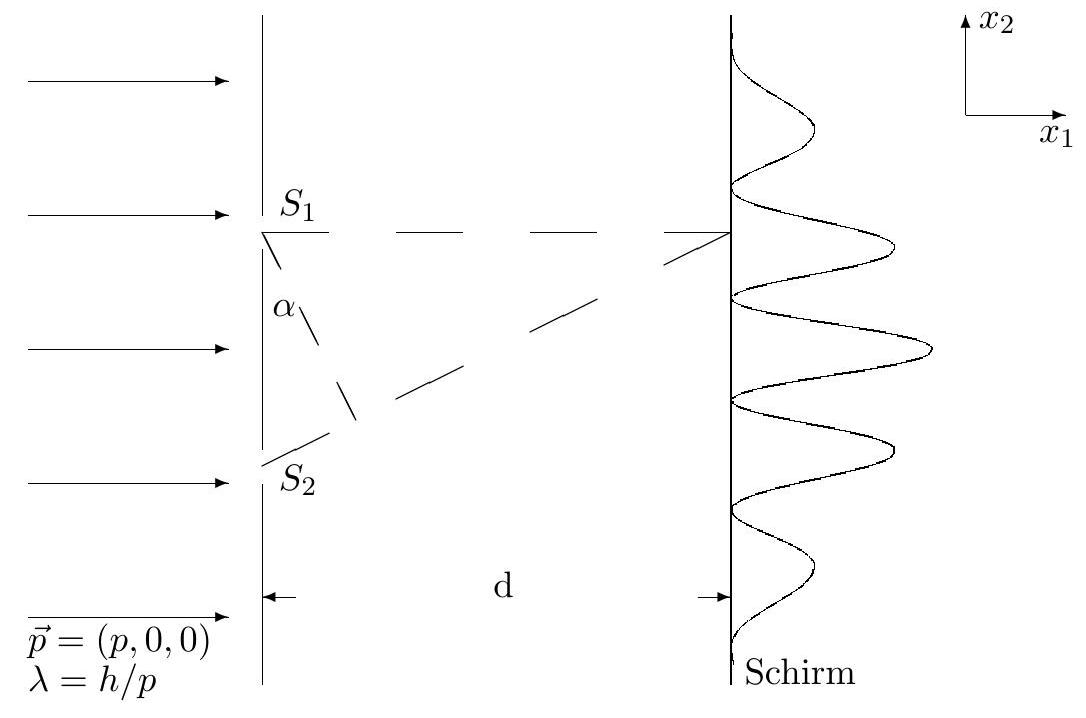
\includegraphics[scale=0.2, center]{2025_05_21_11b1754c718f6fcf84f8g-19}

Von links fällt eine ebene Welle mit Frequenz $\omega=\frac{E}{\hbar}=\frac{1}{\hbar}\left(\frac{1}{2 m} \vec{p}^{2}\right)$ und Wellenvektor $\vec{k}=\frac{1}{\hbar} \vec{p}$ auf eine Blende mit den Spalten $S_{1}$ und $S_{2}$, die sich im Abstand $a$ voneinander befinden. Die Spalten sind kohärente Quellen für die Kugelwellen ${ }^{9}$

$$
A_{1} \frac{e^{-i(\omega t-k|\vec{x}-\vec{a} / 2|)}}{|\vec{x}-\vec{a} / 2|}, \quad A_{2} \frac{e^{-i(\omega t-k|\vec{x}+\vec{a} / 2|)}}{|\vec{x}+\vec{a} / 2|}, \quad k=|\vec{k}|=\frac{2 \pi}{\lambda}
$$

die sich hinter der Blende überlagern:

$$
\psi(\vec{x}, t)=A_{1} \frac{e^{-i(\omega t-k|\vec{x}-\vec{a} / 2|)}}{|\vec{x}-\vec{a} / 2|}+A_{2} \frac{e^{-i(\omega t-k|\vec{x}+\vec{a} / 2|)}}{|\vec{x}+\vec{a} / 2|}
$$

Die zugehörige Intensität (unnormierte Wahrscheinlichkeitsdichte) ist

$$
|\psi(\vec{x}, t)|^{2}=\frac{\left|A_{1}\right|^{2}}{(\vec{x}-\vec{a} / 2)^{2}}+\frac{\left|A_{2}\right|^{2}}{(\vec{x}+\vec{a} / 2)^{2}}+\Re e\left(\frac{2 A_{1} A_{2}^{*} e^{i k(|\vec{x}-\vec{a} / 2|-|\vec{x}+\vec{a} / 2|)}}{|\vec{x}-\vec{a} / 2||\vec{x}+\vec{a} / 2|}\right)
$$

Der letzte Term ist für die Interferenzen auf dem Schirm verantwortlich, welche als Funktion der Gangdiffernez $\Delta x=|\vec{x}-\vec{a} / 2|-|\vec{x}+\vec{a} / 2|$ auftreten. Letzter lässt sich via $\Delta x=a \sin \alpha$ durch den Winkel $\alpha$ (siehe Abbildung) ausdrücken.

\section*{Wellen-Bild}
Die Interferenz-Maxima treten beim Doppelspaltexeriment auf wenn die Gangdiffernz $\Delta x$ ein Vielfaches der Wellenlänge $\lambda=2 \pi / k$ ist, also wenn

$$
a \sin \alpha_{n}=n \lambda
$$

gilt. Die Abstände der Maxima betragen auf dem Schirm

$$
d \sin \alpha_{n+1}-d \sin \alpha_{n} \approx \frac{d \lambda}{a}
$$

Hält man einen Spalt zu, so verschwindet das zugehörige $A_{i}$ und ebenso das Interferenzbild.

\section*{Ein-Teilchen Interferenz}
Die Interferenz verschwindet nicht, wenn man die Intensität des einfallenden Elektronenstrahl so stark verringert, daß immer nur ein einziges Elektron gleichzeitig in der Apparatur ist. Für eine genügende Statistik ist die Messung dann natürlich viele Male zu wiederholen.

\section*{Einzelne Elektronen interferieren mit sich selber.}
Dies ist für alle Materiewellen der Fall. Da Elementarteilchen vom selben Typus ununterscheidbar sind, ist diese Aussage für den Viel-Teilchen Fall zu spezifizieren.

\footnotetext{${ }^{9}$ Für die Theorie von Kugelwellen verweisen wir auf die Elektrodynamik.
}\subsection*{Ehrenfest Theorem}
\subsubsection*{Hermitisch konjungierte Operatoren}
Mit $A^{\dagger}$ bezeichnet man den zu $A$ hermitisch konjungierten Operator. In Matrix Notation transponiert man die Matrix und nimmt dann die komplex-konjungierte Werte

$$
A \hat{=} A_{i j}, \quad\left(A^{\dagger}\right)_{i j}=A_{j i}^{*}
$$

Es folgt

$$
(A \psi)^{*}=\psi^{*} A^{\dagger}
$$

was sich in Matrix-Notation mit $\psi=\left(\psi_{1}, \psi_{2}, \ldots\right)$ einfach nachvollziehen lässt:

$$
(A \psi)_{i}=\sum_{k} A_{i k} \psi_{k}, \quad\left((A \psi)^{*}\right)_{i}=\sum_{k} A_{i k}^{*} \psi_{k}^{*}=\sum_{k}\left(A^{\dagger}\right)_{k i} \psi_{k}^{*}=\left(\psi^{*} A^{\dagger}\right)_{i}
$$

q.e.d. Angewandt auf die Schrödinger-Gleichung folgt

$$
i \hbar \dot{\psi}=H \psi, \quad-i \hbar \dot{\psi}^{*}=\psi^{*} H^{\dagger}=\psi^{*} H
$$

letzteres da der Hamilton-Operator symmetrisch und reel is, und damit selbst-adjungiert, d.h. es gilt $H=H^{\dagger}$.

\subsubsection*{Bewegungsgleichung für Erwartungswerte}
Die zeitliche Entwicklung von eines Erwartungwerts $\langle A\rangle$ is durch

$$
i \hbar \frac{d}{d t}\langle A\rangle=i \hbar \frac{d}{d t} \int d^{3} x \psi^{*} A \psi=\int d^{3} x \psi^{*} A(H \psi)-\int d^{3} x\left(\psi^{*} H\right) A \psi
$$

gegeben. Für den ersten Term haben wir die Schrödinger Gleichung $i \hbar \dot{\psi}=H \psi$ verwendet, und im zweiten Term die komplex-konjungierte Schrödinger Gleichung $-i \hbar \dot{\psi}^{*}=\psi^{*} H$. Hier haben wir angenommen, dass der Operator $A$ selber nicht explizit von der Zeit abhängt. Sollte das der Fall sein, ergibt sich insgesamt

$$
i \hbar \frac{d}{d t}\langle A\rangle=\langle[A, H]\rangle+i \hbar\left\langle\frac{\partial A}{\partial t}\right\rangle
$$

was man als Ehrenfest Theorem bezeichnet. Den Kommutator $[A, H]=A H-H A$ hatten wir bereits eingeführt.

\subsubsection*{Quasiklassische Bewegung}
Wir wenden das Ehrenfest Theorem auf den Impuls- und den Orts-Operator an. Für ein Teilchen in einem Zeit-unabhängignen Potential $V(x)$ gilt

$$
H=\frac{p^{2}}{2 m}+V(x), \quad[p, H]=[p, V(x)], \quad[x, H]=\left[x, p^{2}\right] / 2 m
$$

da Operatoren mit sich selber vertauschen. Der erste Term ergibt

$$
[p, H]=\frac{\hbar}{i}\left(\nabla_{x} V(x)-V(x) \nabla_{x}\right)=\frac{\hbar}{i} V^{\prime}
$$

während wir den zweiten Term mit Hilfe von $[x, p]=i \hbar$ zu

$$
\left[x, p^{2}\right]=x p^{2}-p^{2} x=(x p-p x+p x) p-p^{2} x=i \hbar p+p[x, p]=2 i \hbar p
$$

umformen. In das Ehrenfest Theorem eingesetzt finden wir

$$
i \hbar \frac{d}{d t}\langle p\rangle=\frac{\hbar}{i}\left\langle V^{\prime}\right\rangle, \quad i \hbar \frac{d}{d t}\langle x\rangle=\frac{i \hbar}{m}\langle p\rangle
$$

was zusammen

$$
m \frac{d}{d t}\langle x\rangle=\langle p\rangle \quad \frac{d}{d t}\langle p\rangle=-\left\langle V^{\prime}\right\rangle
$$

ergibt. Die Erwartungswerte von Operatoren gehorchen also den klassischen Bewegungsgleichungen. Dieses ist allerding nicht verwunderlich, da die Schrödinger-Gleichung dem Korrespondenzprinzip genügt.


\pagebreak


\section{Eindimensionale Systeme}
\subsection*{Stationäre Schrödinger-Gleichung}
\section*{Seperation der Variabeln}
Ist das Potential $V(\vec{x})$ von der Zeit $t$ unabhängig, so kann man für die zeitabhängige Schrödinger-Gleichung $i \hbar \dot{\psi}(\vec{x}, t)=H \psi(\vec{x}, t)$ nach Lösungen der Form

$$
\psi(\vec{x}, t)=\sigma(t) u(\vec{x})
$$

suchen (Separation der Variablen). Dies führt zu

$$
i \hbar u(\vec{x}) \frac{d}{d t} \sigma(t)=\left[-\frac{\hbar^{2}}{2 m_{e}} \Delta u(\vec{x})+V(\vec{x}) u(\vec{x})\right] \sigma(t)
$$

Dividiert man durch $\sigma(t) u(\vec{x}) \neq 0$, so erhält man

$$
i \hbar \frac{1}{\sigma(t)} \frac{d \sigma(t)}{d t}=\frac{1}{u(\vec{x})} \mathbf{H} u(\vec{x}), \quad \mathbf{H}=-\frac{\hbar^{2}}{2 m_{e}} \Delta+V(\vec{x})
$$

Da die linke Seite eine Funktion der unabhängigen Variablen $t$, die rechte Seite eine Funktion der unabhängigen Variablen $\vec{x}$ ist, muß

$$
i \hbar \frac{1}{\sigma(t)} \frac{d \sigma(t)}{d t}=E=\mathrm{const}
$$

gelten, d.h.

$$
\sigma(t)=C e^{-i E t / \hbar}, \quad C=\text { const. }
$$

und

$$
\mathbf{H} u(\vec{x})=\left(-\frac{\hbar^{2}}{2 m_{e}} \Delta u(\vec{x})+V(\vec{x}) u(\vec{x})\right)=E u(\vec{x})
$$

Dies ist die zeitunabhängige oder stationäre Schrödinger-Gleichung. Die stationäre SchrödingerGleichung hat die Form einer Eigenwert-Gleichung.

\section*{Eigenwerte und Eigenfunktionen}
Sei A eine $n \times n$ Matrix in einem $n$-dimensionalen Vektorraum, und $\vec{v}$ ein $n$ dimensionaler Vektor mit der Eigenschaft

$$
\mathbf{A} \vec{v}=a \vec{v}, \quad a \in \mathbb{R}
$$

so ist $a$ ein Eigenwert von $\mathbf{A}$ und $\vec{v}$ ein Eigenvektor von A zum Eigenwert $a: \vec{v}=\vec{v}_{a}$. Analog ist mit

$$
u(\vec{x})=u_{E}(\vec{x}), \quad \mathbf{H} u_{E}(\vec{x})=E u_{E}(\vec{x})
$$

$u(\vec{x})$ eine Eigenfunktion des Schrödinger-Operators H, hier zum Eigenwert E.

\section*{Überlagerung zweier Lösungen}
Seien $\psi_{j}(\vec{x}, t)=\sigma_{j}(t) u_{E_{j}}(\vec{x})$ zwei Lösungen der Schrödinger-Gleichung, mit

$$
\sigma_{j}(t)=C_{j} e^{-i E_{j} t / \hbar} \quad \text { und } \quad u_{E_{j}}(\vec{x}), \quad j=1,2,
$$

so ist auch jede linear Superposition von $\psi_{1}$ und $\psi_{2}$ eine Lösung. Das heisst, es gilt

$$
i \hbar \partial_{t} \psi(\vec{x}, t)=\mathbf{H} \psi(\vec{x}, t), \quad \psi(\vec{x}, t)=\alpha_{1} \psi_{1}(\vec{x}, t)+\alpha_{2} \psi_{2}(\vec{x}, t),
$$

mit konstanten $\alpha_{j}$.

\section*{Eigenwert-Spektren}
Die Eigenwerte des Hamilton-Operators können diskret oder kontinuierlich sein:

$$
\begin{aligned}
-\infty<E_{1}, \ldots, E_{\nu}, \ldots & \text { diskrete Eigenwerte, } \\
\{-\infty<E<\infty\} & \text { kontinuierlich verteilte Eigenwerte. }
\end{aligned}
$$

Wegen der Linearität der Schrödinger-Gleichung sind beliebige Überlagerungen

$$
\psi(\vec{x}, t)=\sum_{\nu=1}^{\infty} C_{\nu} e^{-i E_{\nu} t / \hbar} u_{E_{\nu}}(\vec{x})+\int d E C(E) e^{-i E t / \hbar} u_{E}(\vec{x})
$$

der orthonomierten Eigenfunktionen $u_{E_{\nu}}(\vec{x})$ und $u_{E}(\vec{x})$ wiederum Lösungen von $\mathbf{H}$, mit $C_{\nu} \in \mathcal{C}$ und $C(E) \in \mathcal{C}$ und der Bedingung für die Normierung der Wellefunktion,

$$
\sum_{\nu}\left|C_{\nu}\right|^{2}+\int d E|C(E)|^{2}=1
$$

Man beachte, dass die Energie unten beschränkt sein muss, da das System sonst nicht stabil ist: $E \geq B>-\infty$.

\section*{Eigenfunktionen des Impulsoperators}
Als Beispiel betrachten wir die Eigenfunktionen $e_{p}(x)$ des Impulsoperators $\mathbf{P}=\frac{\hbar}{i} \frac{d}{d x}$ zum reellen Eigenwert $p$ :

$$
\mathbf{P} e_{p}(x)=\frac{\hbar}{i} \frac{d}{d x} e_{p}(x)=p e_{p}(x)
$$

Die Eigenlösungen sind offenbar $e_{p}(x)=C e^{i p x / \hbar}$, mit $C=$ const., also ebene Wellen.

\subsection*{Eindimensionale Potentialstufe}
Wir betrachten das eindimensionale Potential

$$
\begin{array}{rlll}
V(x)=0 & \text { für } & x<0 \\
V(x)=V_{0}>0 & \text { für } & x>0
\end{array}
$$

Die zugehörige zeitunabhängige Schrödinger-Gleichung zum Eigenwerte $E$ lautet

$$
-\frac{\hbar^{2}}{2 m} \frac{d^{2} u(x)}{d x^{2}}+V(x) u(x)=E u(x)
$$

\section*{Stetigkeits-Bedingungen am Potentialsprung}
Das Potential springt bei $x=0 \mathrm{um} V_{0}$. Dahe stellt sich die Frage, ob die Wellenfunktion auch Diskontinuitäten aufweist. Aus

$$
\frac{d^{2} u(x)}{d x^{2}}=-\frac{2 m}{\hbar^{2}}(E-V) u(x)
$$

folgt, daß bei stetigem $u(x)$ die zweite Ableitung von $u$ (linke Seite) bei $x=0$ einen endlichen Sprung um $2 m V_{0} / \hbar^{2} u(0)$ macht.

Die erste Ableitung $d u / d x$ ist dagegen stetig:

$$
\begin{aligned}
\lim _{\epsilon \rightarrow 0}\left(\left.\frac{d u}{d x}\right|_{\epsilon}-\left.\frac{d u}{d x}\right|_{-\epsilon}\right) & =\lim _{\epsilon \rightarrow 0} \int_{-\epsilon}^{+\epsilon} d x \frac{d}{d x}\left(\frac{d u}{d x}\right) \\
& =\lim _{\epsilon \rightarrow 0}-\frac{2 m}{\hbar^{2}} \int_{-\epsilon}^{+\epsilon} d x(E-V) u(x)=0
\end{aligned}
$$

da der Integrand endlich ist und das Integrationsintervall gegen Null tendiert.\\
Die Anschlussbedingung für $x=0$ ist also: $u(x)$ und $u^{\prime}(x)$ sind stetig. Allgemein spricht man auch von Randbedingungen.

\subsubsection*{Streuzustände}
Wenn das Potential konstant ist, $V=0$ oder $V=V_{0}$, wird die stationäre-Schrödinger Gleichung durch ebene Wellen gelöst:

$$
u(x)=e^{ \pm i k x}, \quad \frac{(\hbar k)^{2}}{2 m}=E-V
$$

modulo einer Normierungskontanten. Dabei enspricht $+k$ und $-k$ links-, bzw. rechtslaufenden Wellen.

\section*{Einlaufende und reflektierte Welle}
Wir betrachten $E>V_{0}$, die Eigenenergie des Zustandes ist also größer als die Potentialstufe. Klassisch würde ein von links einfallendews Elektron daher einfach durchlaufen. Um festzustellen, ob dies auch quantenmechanisch der Fall ist, gehen wir von der allgemeinen Lösung aus. D.h. wir betrachten $x \leq 0$ und

$$
x \leq 0: \quad u(x)=e^{i k x}+R e^{-i k x}, \quad k=\frac{1}{\hbar} \sqrt{2 m E}>0
$$

also eine allgemeine Superposition von einlaufender und reflektierte Welle. Zur einlaufenden Welle $(+k)$ wird die rücklaufende Welle $(-k)$ mit Amplitude $R$ zugemischt. Der entsprechende Teilchenfluss (die Wahrscheinlichkeits-Stromdichte) ist

$$
s(x)=\frac{\hbar}{2 m i}\left(u^{*} \frac{d u}{d x}-u \frac{d u^{*}}{d x}\right), \quad s_{-}=\frac{\hbar k}{m}\left(1-|R|^{2}\right)
$$

da sich die Mischterme gegenseitig aufheben.

\begin{itemize}
  \item $e^{i k x}$ beschreibt eine von links einfallende Welle mit Fluss $\hbar k / m>0$
  \item $R e^{-i k x}$ beschreibt eine an der Stufe reflektierte Welle mit Fluss $-|R|^{2} \hbar k / m$.
\end{itemize}

Die Anschlussbedingung bei $x=0$ bestimmt dabei $R$.

\section*{Transmitierte Welle}
Die Lösung für $x \geq 0$ lautet

$$
x \geq 0: \quad u(x)=T e^{i q x}, \quad q=\frac{1}{\hbar} \sqrt{2 m\left(E-V_{0}\right)}, \quad s_{+}=\frac{\hbar q}{m}|T|^{2}
$$

Die ebenfalls mögliche Lösung $e^{-i q x}$ lassen wir weg, da von rechts keine Welle einfallen soll. $s_{+}=\frac{\hbar q}{m}|T|^{2}$ ist der nach rechts durchlaufende Strom.

\begin{center}
\begin{tabular}{ccl}
\hline
Welle & Fluss & Interpretation \\
\hline
$e^{i k x}$ & $\hbar k / m$ & Einlaufende Welle \\
$R e^{-i k x}$ & $-|R|^{2} \hbar k / m$ & $R$ : Reflektions-Koeffizient \\
$T e^{i q x}$ & $|T|^{2} \hbar q / m$ & $T$ : Transmissions-Koeffizient \\
\hline
\end{tabular}
\end{center}

\section*{Stetigkeitsbedingungen}
$\overline{u(x) \text { ist bei } x=0 \text { nur dann stetig wenn }}$

$$
1+R=T
$$

erfüllt is. Analog ist die Ableitung $d u / d x$ bei $x=0$ stetig falls

$$
i k(1-R)=i q T
$$

gilt. Zusammen folgt

$$
R=\frac{k-q}{k+q}, \quad T=\frac{2 k}{k+q}
$$

Damit sind $R$ und $T$ als Funktionen von $E$ und $V_{0}$ bekannt.

\section*{Teilchenstromerhaltung}
Man rechnet unmittelbar nach, dass

$$
\frac{\hbar k}{m}\left(1-|R|^{2}\right)=\frac{\hbar q}{m}|T|^{2}
$$

gilt. Damit is $s(x)$ ebenfalls bei $x=0$ stetig. Das war zu erwarten, da der Teilchenstrom aufgrund der Kontinuitätsgleichung erhalten ist.

Im Gegensatz zur klassischen Mechanik, für die für $E>V_{0}$ kein Teilchen an der Potentialstufe reflektiert würde, wird in der Quantenmechanik ein endliche Bruchteil, $|R|^{2}$, des Elektrons reflektiert.

\subsubsection*{Reflektierte Zustände}
Wir betrachten nun $E<V_{0}$. Für $x \leq 0$ ist die allgemeie Lösung durch

$$
x \leq 0: \quad u(x)=A_{1} \sin k x+B_{1} \cos k x, \quad k=\frac{1}{\hbar} \sqrt{2 m E}
$$

gegeben, für $x \geq 0$ analog durch

$$
x \geq 0: \quad u(x)=A_{2} e^{-\kappa x}+B_{2} e^{\kappa x}, \quad \kappa=\frac{1}{\hbar} \sqrt{2 m\left(V_{0}-E\right)}
$$

Aus physikalischen Gründen (Normierbarkeit) kann $u(x)$ für $x>0$ nicht beliebig groß werden, woraus $B_{2}=0$ folgt.

\section*{Stetigkeitsbedingungen}
Die Bedingung der Stetigkeit von $u(x)$ und von $d u / d x$ für $x=0$ ergibt

$$
A_{2}=B_{1}, \quad A_{1} k=-A_{2},
$$

woraus

$$
\begin{array}{ll}
x \leq 0: & u(x)=A_{1}\left(\sin k x-\frac{k}{\kappa} \cos k x\right) \\
x \geq 0: & u(x)=-A_{1} \frac{k}{\kappa} e^{-\kappa x}
\end{array}
$$

folgt.

\section*{Bemerkungen}
\begin{itemize}
  \item Es ist überall $s(x)=0$. Stehende Wellen transportieren keine Teilchen.
  \item Im Gegensatz zum klassischen Fall dringt ein Bruchteil der Teilchen auch in das "verbotene" Gebiet $x>0$ ein. Im klassisch verbotenem Bereich fällt die Teilchendichte $|u(x)|^{2}$ exponentiell ab, mit der Eindringstiefe
\end{itemize}

$$
\lambda=\frac{1}{2 \kappa}=\frac{\hbar / 2}{\sqrt{2 m\left(V_{0}-E\right)}}
$$

Diese Phänomene werden an allen Grenzflächen beobachtet, sie sind u.A. in der Halbleiterphysik von Bedeutung.

\subsection*{Potentialbarriere}
\begin{center}
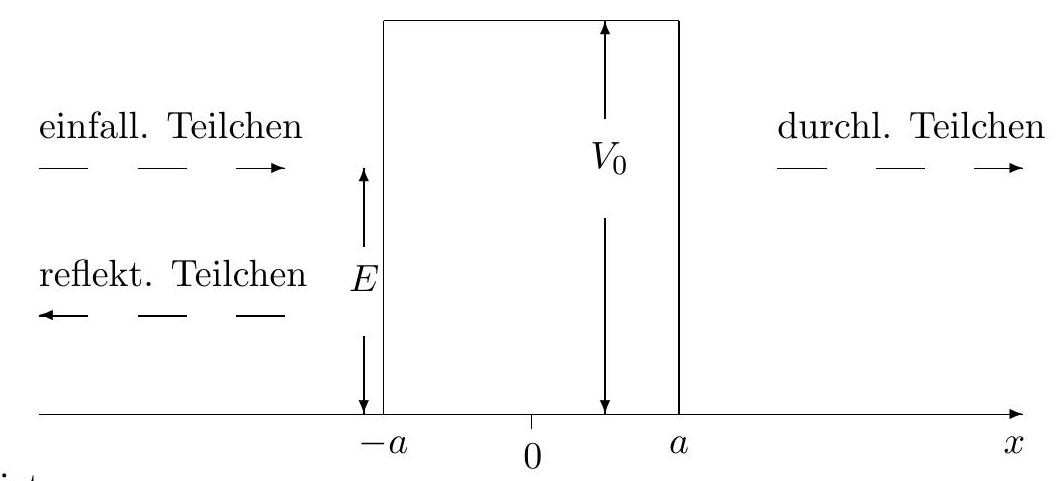
\includegraphics[scale=0.2]{2025_05_21_2790b5a0182e53887e3bg-08}
\end{center}

Das Potential ist:

$$
V(x)=\left\{\begin{array}{llc}
0 & \text { für } & x<-a \\
V_{0}>0 & \text { für } & -a<x<a \\
0 & \text { für } & x>a
\end{array}\right.
$$

\section*{Wellenfunktion}
Wir nehmen an, dass von links Teilchen mit der Energie $E<V_{0}$ einfallen und zum Teil reflektiert werden. Von rechts sollen keine Teilchen einfallen. Wir haben somit

$$
\begin{aligned}
x<-a: & u(x) & =e^{i k x}+R e^{-i k x} & \\
-a<x<a: & u(x) & =A e^{-\kappa x}+B e^{\kappa x} & \\
x>a: & u(x) & =T e^{i k x} . &
\end{aligned}
$$

\section*{Stetigkeitsbedingungen}
Die Stetigkeit von $u(x)$ und $d u / d x$ bei $x= \pm a$ führt auf folgendes lineare Gleichungssystem, für die vier Grössen $R, A, B$ und $T$ :

$$
\begin{aligned}
& x=-a:\left\{\begin{aligned}
& e^{-i k a}+R e^{i k a}=A e^{\kappa a}+B e^{-\kappa a} \\
& i k\left(e^{-i k a}-R e^{i k a}\right)= \\
&\left.x=+a:-A e^{\kappa a}+B e^{-\kappa a}\right) \\
& A e^{-\kappa a}+B e^{\kappa a}=T e^{i k a} \\
& \kappa\left(-A e^{-\kappa a}+B e^{\kappa a}\right)=i k T e^{i k a}
\end{aligned}\right.
\end{aligned}
$$

Aus den beiden ersten Gleichungen ergibt sich

$$
\begin{aligned}
2 A e^{\kappa a} & =\left(1-i \frac{k}{\kappa}\right) e^{-i k a}+R\left(1+i \frac{k}{\kappa}\right) e^{i k a} \\
2 B e^{-\kappa a} & =\left(1+i \frac{k}{\kappa}\right) e^{-i k a}+R\left(1-i \frac{k}{\kappa}\right) e^{i k a}
\end{aligned}
$$

durch Addition und Subtraktion; ebenso aus den beiden letzten Gleichungen:

$$
\begin{aligned}
2 A e^{-\kappa a} & =\left(1-i \frac{k}{\kappa}\right) e^{i k a} T \\
2 B e^{\kappa a} & =\left(1+i \frac{k}{\kappa}\right) e^{i k a} T
\end{aligned}
$$

Die Quotienten führen zu

$$
\frac{A}{B}=\frac{\left(1-i \frac{k}{\kappa}\right) e^{-i k a}+R\left(1+i \frac{k}{\kappa}\right) e^{i k a}}{\left(1+i \frac{k}{\kappa}\right) e^{-i k a}+R\left(1-i \frac{k}{\kappa}\right) e^{i k a}} e^{-2 \kappa a}=\frac{\left(1-i \frac{k}{\kappa}\right) e^{i k a}}{\left(1+i \frac{k}{\kappa}\right) e^{i k a}} e^{2 \kappa a} .
$$

Mit $\rho=k / \kappa$ erhalten wir hieraus

$$
\left[\left(1+\rho^{2}\right) e^{-2 i k a}+R(1+i \rho)^{2}\right] e^{-2 \kappa a}=\left[\left(1+\rho^{2}\right) e^{-2 i k a}+R(1-i \rho)^{2}\right] e^{2 \kappa a}
$$

oder

$$
\left(1+\rho^{2}\right) e^{-2 i k a} \sinh (2 \kappa a)=R\left[\left(1+2 i \rho-\rho^{2}\right) e^{-2 \kappa a}-\left(1-2 i \rho-\rho^{2}\right) e^{2 \kappa a}\right]
$$

Setzen wir dies in den Quotienten aus den ersten beiden Gleichungen ein, so ergibt sich:

$$
R=e^{-2 i k a} \frac{\left(\kappa^{2}+k^{2}\right) \sinh (2 \kappa a)}{\left(k^{2}-\kappa^{2}\right) \sinh (2 \kappa a)+2 i \kappa k \cosh (2 a \kappa)}
$$

Analog findet man

$$
T=e^{-2 i k a} \frac{2 i \kappa k}{\left(k^{2}-\kappa^{2}\right) \sinh (2 \kappa a)+2 i \kappa k \cosh (2 a \kappa)}
$$

Daraus bekommt man folgende Absolutquadrate:

$$
\begin{aligned}
|R|^{2} & =\frac{\left(\kappa^{2}+k^{2}\right)^{2} \sinh ^{2}(2 \kappa a)}{\left(\kappa^{2}-k^{2}\right)^{2} \sinh ^{2}(2 \kappa a)+4 \kappa^{2} k^{2} \cosh ^{2}(2 \kappa a)} \\
|T|^{2} & =\frac{4 \kappa^{2} k^{2}}{\left(\kappa^{2}-k^{2}\right)^{2} \sinh ^{2}(2 \kappa a)+4 \kappa^{2} k^{2} \cosh ^{2}(2 \kappa a)}
\end{aligned}
$$

d.h. $|R|^{2}+|T|^{2}=1$, denn $\cosh ^{2}-\sinh ^{2}=1$.

\section*{Tunneleffekt}
Obwohl $E<V_{0}$ können Teilchen durch die Barriere tunneln, wobei vor allem die Größe

$$
\kappa a=\frac{1}{\hbar} \sqrt{2 m a^{2}\left(V_{0}-E\right)}
$$

für den Bruchteil der durchlaufenden Elektronen verantwortlich ist.

\section*{Klassischer Grenzfall}
Wir betrachten nun den Fall kleiner Tunnelwahrscheinlichkeit, also z.B. $E \ll V_{0}$ oder allg.

$$
\kappa a \gg 1: \quad \sinh (2 \kappa a) \approx \frac{1}{2} e^{+2 \kappa a},
$$

d.h.

$$
|T|^{2} \approx \frac{(4 \kappa k)^{2}}{\left(\kappa^{2}+k^{2}\right)^{2}} e^{-4 \kappa a} \quad \kappa a=\frac{1}{\hbar} \sqrt{2 m a^{2}\left(V_{0}-E\right)}
$$

Wir bemerken, daß im klassischen Grenzfall $\hbar \rightarrow 0$ das Produkt $\kappa a$ divergiert, mit $\kappa a \rightarrow$ $\infty$, die Tunnelrate ist daher exponentiell unterdrückt.

\section*{Allgemeine Tunnelbarriere}
Ein allgemeines Tunnelpotential $V(x)$ kann man näherungsweise im klassichen Grenzfall behandeln. Dafür berücksichtigt man in obiger Formel nur die Exponentialfunktion, womit die Transmissionskoeffizienten näherungsweise multiplikativ sind. Teilen wir die Barriere in kleine Abschnitte, $a=a_{1}+a_{2}+\ldots$, dann gilt für die zugehörigen Transmissionskoeffizienten

$$
\left|T_{a}\right|^{2} \approx\left|T_{a_{1}}\right|^{2} \cdot\left|T_{a_{2}}\right|^{2} \cdot \ldots
$$

(Multiplikationssatz der Wahrscheinlichkeiten).\\
Approximiert man einen kontinuierlichen Potentialberg $V(x)$ durch immer kleinere Stufen der Dicke $a_{i}$, so erhält man, abgesehen von einem Normierungsfaktor,

$$
|T| \approx e^{-2 \int d x \sqrt{\left(2 m / \hbar^{2}\right)(V(x)-E)}}
$$

Der Tunneleffekt ist ein wichtiges physikalischen Phänomen. Er ist z.B. für den Kernzerfall sowie für die kalte Emission von Elektronen aus einer Metalloberfläche (Kathode) verantwortlich.\\
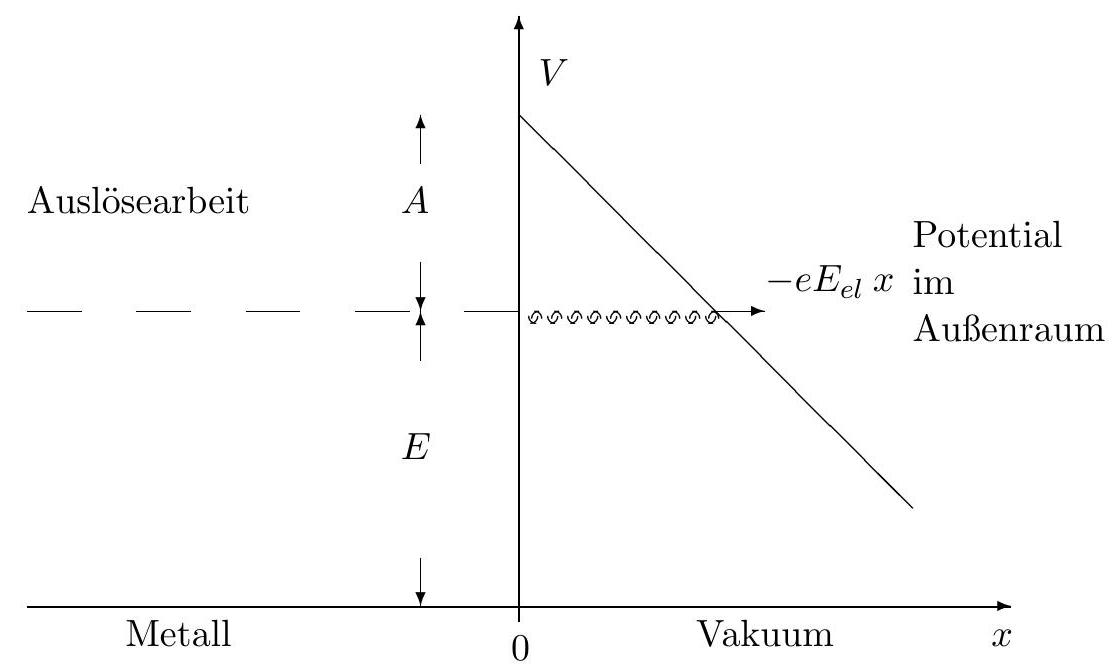
\includegraphics[scale=0.2, center]{2025_05_21_2790b5a0182e53887e3bg-11}

\subsection*{Unendlich tiefer Potentialtopf}
Wir studieren nun den Potentialverlauf

$$
\begin{array}{ll}
V(x)=0 & \text { für }-a<x<a \\
V(x)=\infty & \text { sonst }
\end{array}
$$

In Kap. 2.2 haben wir gesehen, daß die Wellenfunktion mit Energie $E<V_{0}$ in der Potentialstufe exponentiell unterdrückt wird. Für den unendlich tiefen Potentialtopf, mit $V_{0} \rightarrow \infty$, folgt also dass $u(x)=0$ für $|x| \geq a$ gilt. Im Topf selbst hat man

$$
\frac{d^{2} u}{d x^{2}}=-\frac{2 m E}{\hbar^{2}} u
$$

Keine Lösungen für $E<0$\\
Falls $E<0$ ist, so hat man für $-a<x<a$ die Lösungen

$$
u(x)=A_{1} e^{\kappa x}+A_{2} e^{-\kappa x}, \quad \kappa=\frac{1}{\hbar}(-2 m E)^{\frac{1}{2}}
$$

mit denen man die Randbedingungen $u(a)=u(-a)=0$ jedoch nur mit $A_{1}=A_{2}=0$ erfüllen kann. Es gibt also keine Lösungen für das Problem mit $E<0$.

\section*{Lösungen für $E>0$}
Für $E>0$ gilt

$$
\frac{d^{2} u}{d x^{2}}=-k^{2} u(x), \quad k=\frac{1}{\hbar} \sqrt{2 m E}
$$

für $-a<x<a$, mit den Lösungen

$$
\begin{array}{ll}
u^{(-)}(x)=A^{(-)} \sin k x & (\text { ungerade Funktion in } x) \\
u^{(+)}(x)=A^{(+)} \cos k x & (\text { gerade Funktion in } x)
\end{array}
$$

\section*{Antisymmetrische Lösung}
Aus der Randbedingung $\sin (a x)=0$ für die ungerade (antisymmetrische) Lösung folgt $k a=n \pi$, mit $n=1,2,3, \ldots$. Es sind also nur diskrete (bestimmte) Werte von $k$ (und damit der Energie E) mit der Randbedingung vertäglich. Die Eigenwerte sind somit quantisiert.

Die zulässigen Energiewerte sind

$$
E_{n}^{(-)}=\frac{n^{2} \pi^{2} \hbar^{2}}{2 m a^{2}}, \quad n=1,2,3, \ldots
$$

Die Normierung der zugehörigen Eigenfunktionen

$$
u_{n}^{(-)}=A^{(-)} \sin \left(\frac{n \pi x}{a}\right)
$$

gemäß $\int_{-a}^{a} u^{*}(x) u(x) d x=1$ ergibt $A^{(-)}=(a)^{-\frac{1}{2}}$, also

$$
u_{n}^{(-)}(x)=a^{-\frac{1}{2}} \sin \left(\frac{n \pi x}{a}\right), \quad n=1,2,3, \ldots
$$

\section*{Symmetrische Lösung}
Für die gerade (symmetrische) Lösung folgt aus $\cos k a=0$, dass hier $k a=(n+1 / 2) \pi$ gilt, wobei $n$ eine ganze Zahl ist. Damit lauten die Eigenwerte

$$
E_{n}^{(+)}=\frac{(n+1 / 2)^{2} \pi^{2} \hbar^{2}}{2 m a^{2}}, \quad n=0,1,2, \ldots
$$

Die zugehörigen (normierten) Eigenfunktionen sind

$$
u_{n}^{(+)}=a^{-\frac{1}{2}} \cos \left[(n+1 / 2) \frac{\pi x}{a}\right], \quad n=0,1,2, \cdots
$$

\section*{rundzustandsenergie}
Der tiefstmögliche Energiewert - die Grundzustandsenergie- ist

$$
E_{n=0}^{(+)}=\frac{\pi^{2} \hbar^{2}}{8 m a^{2}}
$$

Der niedrigste antisymmetriche Zustand, $u_{n=1}^{(-)}(x)$, hat die eine höhre Energie, $E_{n=1}^{(-)}=$ $4 E_{n=0}^{(+)}$.

\section*{Knoten der Wellenfunktion}
Die Energien $E_{n}^{( \pm)}$sind jeweils um so größer, je größer die Zahl der Nullstellen (Knoten)\\
der zugehörigen Eigenfunktionen $u_{n}^{( \pm)}(x)$ im Intervall $[-a,+a]$ ist. Je mehr Knoten, desto schneller verändert sich die Wellefunktion, desto grösser der Gradient, desto grösser damit auch die kinetische Energie.

Die Wellenfunktion $u_{n=0}^{(+)}=a^{-1 / 2} \cos \pi x /(2 a)$ des Grundzustandes hat keine Nullstelle für $|x|<a$.

\section*{Orthogonalität}
Mittels der Beziehungen

$$
\begin{aligned}
2 \cos \alpha_{1} \cos \alpha_{2} & =\cos \left(\alpha_{1}+\alpha_{2}\right)+\cos \left(\alpha_{1}-\alpha_{2}\right) \\
2 \sin \alpha_{1} \sin \alpha_{2} & =\cos \left(\alpha_{1}-\alpha_{2}\right)-\cos \left(\alpha_{1}+\alpha_{2}\right) \\
2 \sin \alpha_{1} \cos \alpha_{2} & =\sin \left(\alpha_{1}+\alpha_{2}\right)+\sin \left(\alpha_{1}-\alpha_{2}\right)
\end{aligned}
$$

erhält man mit $\sigma= \pm$ die Orthogonalitätsbeziehungen

$$
\int_{-a}^{a} d x\left(u_{m}^{(\sigma)}\right)^{*}(x) u_{n}^{(\sigma)}(x)=\delta_{m n}, \quad \int_{-a}^{a} d x\left(u_{m}^{(+)}\right)^{*}(x) u_{n}^{(-)}(x)=0
$$

Eigenfunktionen zu verschiedenen Eigenwerten $E_{n}^{( \pm)}$sind bezügliche des Skalarproduktes

$$
(\psi, \phi)=\int d x \psi^{*}(x) \phi(x)
$$

zueinander orthogonal:

$$
\left(u_{n}^{(\gamma)}, u_{m}^{(\alpha)}\right)=\delta_{n, m} \delta_{\gamma, \delta}, \quad \gamma, \alpha= \pm
$$

Das war zu erwarten, da der Hamilton-Operator symmetrisch ist, und symmetrische Matrizen otrhogonale Eigenfunktionen haben. Mehr dazu später.

\section*{Erwartungswerte}
$\overline{\text { Die Mittelwerte }\langle x\rangle}$ und $\langle p\rangle$ verschwinden. Z.B. ergibt sich

$$
\langle x\rangle=\frac{1}{a} \int_{-a}^{a} d x \sin \left(\frac{n \pi x}{a}\right) x \sin \left(\frac{n \pi x}{a}\right)=0
$$

da der Integrand antisymmetrisch in $x$ ist. Damit reduzieren sich die Schwankungsquadrate zu

$$
(\Delta x)^{2}=\left\langle x^{2}\right\rangle-\langle x\rangle^{2}=\left\langle x^{2}\right\rangle, \quad(\Delta p)^{2}=\left\langle p^{2}\right\rangle-\langle p\rangle^{2}=\left\langle p^{2}\right\rangle
$$

\section*{Impulsunschärfe}
$\overline{\text { Mit } \mathbf{H}=\mathbf{P}^{2} / 2 m}$ und $\mathbf{P}^{2}=\hbar \nabla / i$ gilt

$$
\left\langle p^{2}\right\rangle_{n}^{( \pm)}=2 m E_{n}^{( \pm)}=\int_{-a}^{a} d x u_{n}^{( \pm)}(x)\left(-\hbar^{2} \frac{d^{2}}{d x^{2}}\right) u_{n}^{( \pm)}(x)
$$

für die Impulstunschärfe.

\section*{Ortsunschärfe}
Mit der Substitution $y=\pi x / a$ erhalten wir ferner

$$
\begin{aligned}
\left\langle x^{2}\right\rangle_{n}^{(-)} & =\frac{1}{a} \int_{-a}^{a} d x x^{2} \sin ^{2} \frac{n \pi x}{a} \\
& =\frac{1}{\pi} \int_{-\pi}^{\pi}\left(\frac{a y}{\pi}\right)^{2} \sin ^{2} n y d y
\end{aligned}
$$

für das Schwankungsquadrat des Orts-Operators. Da $\sin ^{2} \alpha=(1-\cos 2 \alpha) / 2$, erhält man nach mehrmaliger partieller Integration

$$
\left\langle x^{2}\right\rangle_{n}^{(-)}=\frac{a^{2}}{3}\left(1-\frac{3}{2 \pi^{2} n^{2}}\right)
$$

\section*{Orts- und Impulsunschärfe}
Für die ungeraden Eigenfunktionen lautet das Gesamtergebnis damit

$$
(\Delta p)_{n}^{(-)}=\frac{n \pi \hbar}{a} ; \quad(\Delta x)_{n}^{(-)}=\frac{a}{\sqrt{3}}\left(1-\frac{3}{2 \pi^{2} n^{2}}\right)^{\frac{1}{2}}
$$

Mit $\cos ^{2} \alpha=(1+\cos 2 \alpha) / 2$ findet man analog

$$
(\Delta p)_{n}^{(+)}=\left(n+\frac{1}{2}\right) \frac{\pi \hbar}{a} ; \quad(\Delta x)_{n}^{(+)}=\frac{a}{\sqrt{3}}\left(1-\frac{3}{2 \pi^{2}\left(n+\frac{1}{2}\right)^{2}}\right)^{\frac{1}{2}}
$$

für die ungeraden Wellenfunktionen.

\section*{Unschärferelationen}
Die Unschärferelationen lauten:

$$
\begin{aligned}
(\Delta x)_{n}^{(-)} \cdot(\Delta p)_{n}^{(-)} & =\frac{\hbar}{\sqrt{3}}\left[n^{2} \pi^{2}-3 / 2\right]^{\frac{1}{2}} \\
(\Delta x)_{n}^{(+)} \cdot(\Delta p)_{n}^{(+)} & =\frac{\hbar}{\sqrt{3}}\left[(n+1 / 2)^{2} \pi^{2}-3 / 2\right]^{\frac{1}{2}}
\end{aligned}
$$

\section*{Minimale Unschärfe}
Das Produkt der Unschärfen $\Delta x \cdot \Delta p$ hängt nicht von $a$ ab und wächst mit $n$. Für den Grundzustand $u_{0}^{(+)}$hat man

$$
(\Delta x)_{0}^{(+)} \cdot(\Delta p)_{0}^{(+)}=\frac{\hbar}{\sqrt{3}}\left(\frac{1}{4} \pi^{2}-\frac{3}{2}\right)^{\frac{1}{2}}=0.568 \hbar>\frac{\hbar}{2}
$$

d.h. die allgemeine Heisenberg'sche Unschärferelation $(\Delta \mathbf{P}) \cdot(\Delta \mathbf{Q})>\hbar / 2$ ist erfüllt.

\subsection*{Potentialtopf mit endlicher Tiefe}
Es sei

$$
V(x)=\left\{\begin{array}{rcr}
0 & \text { für } & |x|>a \\
-V_{0}<0 & \text { für } & \mid x]<a
\end{array}\right.
$$

Die Lösungen zu positiver Energie erhält man durch analytische Fortsetzung ( $\kappa \rightarrow-i \kappa$ ) der Lösungen für die Potentialbarriere (siehe Kap. 2.3).

\section*{Gebundene Zustände}
Die Lösungen zu negativen Energien,

$$
-V_{0}<E<0
$$

ensprechen klassisch gebundenen Zuständen, d.h. für $|x| \gg a$ sollte die Wellenfunktion abfallen. Demnach kommen folgende Lösungen der Schrödinger-Gleichung in Frage:

$$
\begin{array}{rll}
x<-a & : & u(x)=B_{-} e^{\kappa x} \\
-a<x<+a: & u(x)=A_{1} \cos q x+A_{2} \sin q x \\
x>a: & u(x)=B_{+} e^{-\kappa x}
\end{array}
$$

mit

$$
q=\sqrt{2 m\left(V_{0}+E\right)} / \hbar, \quad \kappa=\sqrt{-2 m E} / \hbar
$$

Dabei wurde $E=(\hbar \kappa)^{2} /(2 m)=(\hbar q)^{2} /(2 m)-V_{0}$ verwendet.

\section*{Stetigkeitsbedingungen}
Die Forderung nach Stetigkeit der Wellenfunktion und ihrer Ableitung für $x= \pm a$ gibt die Bedingungen

$$
\begin{aligned}
B_{-} e^{-\kappa a} & =A_{1} \cos q a-A_{2} \sin q a \\
\kappa B_{-} e^{-\kappa a} & =q\left(A_{1} \sin q a+A_{2} \cos q a\right) \\
B_{+} e^{-\kappa a} & =A_{1} \cos q a+A_{2} \sin q a \\
\kappa B_{+} e^{-\kappa a} & =q\left(A_{1} \sin q a-A_{2} \cos q a\right)
\end{aligned}
$$

Hieraus folgt

$$
\kappa=q \frac{A_{1} \sin q a+A_{2} \cos q a}{A_{1} \cos q a-A_{2} \sin q a}=q \frac{A_{1} \sin q a-A_{2} \cos q a}{A_{1} \cos q a+A_{2} \sin q a}
$$

d.h. $A_{1}$ oder $A_{2}$ muss verschwinden. Die Lösungen müssen daher vollständig symmetrische oder antisymmetrisch sein,

$$
u^{(+)}(x)=A_{1} \cos q^{(+)} x, \quad u^{(-)}(x)=A_{2} \sin q^{(-)} x
$$

Später werden wir zeigen, daß dies eine Folge der Symmetrieeigenschaften des HamlitonOperators ist, er ist invariant unter der Spiegelung $x \leftrightarrow-x$.

\section*{Eigenwertgleichungen}
Die Gleichungen

$$
\kappa^{(+)}=q^{(+)} \tan \left(q^{(+)} a\right) \quad \kappa^{(-)}=-q^{(-)} \cot \left(q^{(-)} a\right)
$$

bestimmen die zulässigen Eigenwerte $E^{(+)}$und $E^{(-)}$. Mit $b^{2}=2 m V_{0} a^{2} / \hbar^{2}$, bzw. $y^{( \pm)}=$ $a q^{( \pm)}$, finden wir

$$
\kappa=\frac{\sqrt{2 m}}{\hbar} \sqrt{-E}=\frac{\sqrt{2 m}}{\hbar} \sqrt{V_{0}-\frac{(q \hbar)^{2}}{2 m}}=\frac{1}{a} \sqrt{\frac{2 m V_{0} a^{2}}{\hbar^{2}}-(q a)^{2}}
$$

Die transzendenten Gleichungen

$$
\sqrt{b^{2}-\left(y^{(+)}\right)^{2}} / y^{(+)}=\tan y^{(+)}, \quad \sqrt{b^{2}-\left(y^{(-)}\right)^{2}} / y^{(-)}=-\cot y^{(-)}
$$

bestimmen somit $q^{( \pm)}$und daher auch die Eigenwerte $E^{( \pm)}=\left(\hbar q^{( \pm)}\right)^{2} /(2 m)-V_{0}$. Sie können graphisch gelöst werden.\\
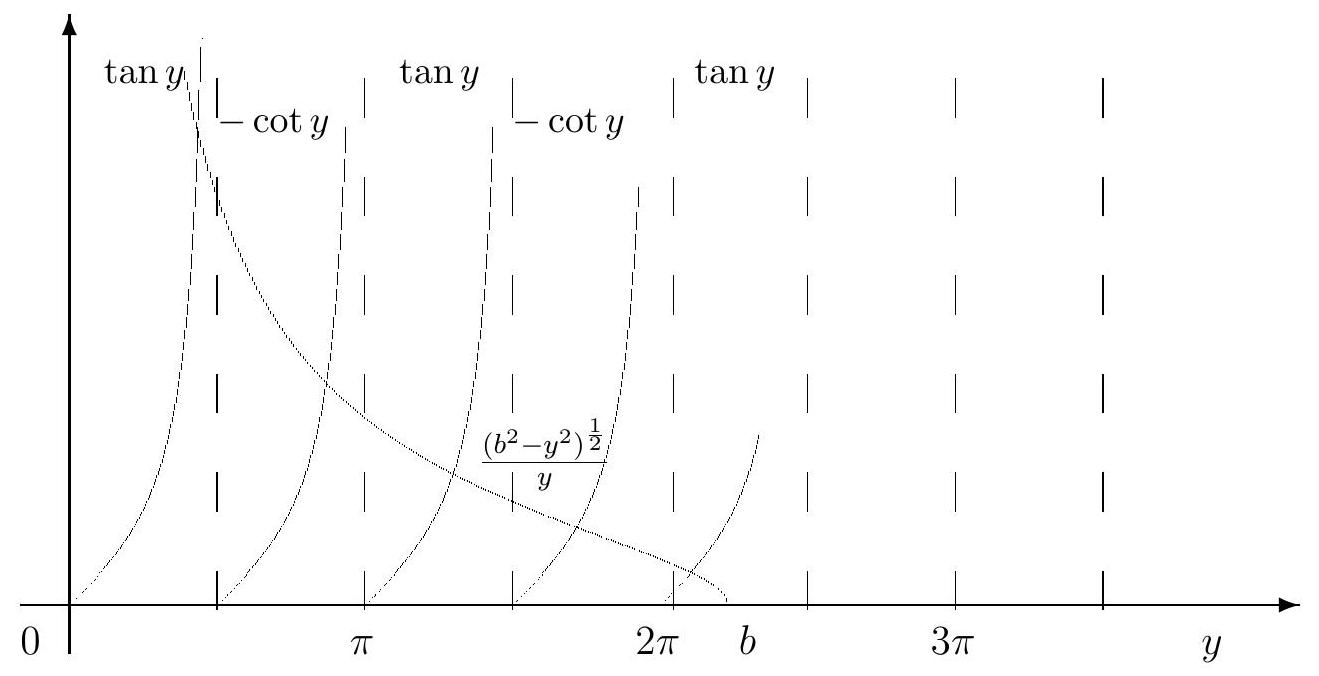
\includegraphics[scale=0.2, center]{2025_05_21_2790b5a0182e53887e3bg-16}

Dabei dievergiert $\tan y=\sin y / \cos y(\cot y=\cos y / \sin y)$ bei $2 \pi$-Vielfachen von $0(\pi / 2$. Die Anzahl der gebundenen Zustände hängt von dem Wert von $b^{2}=2 m V_{0} a^{2} / \hbar^{2} \mathrm{ab}$.

\section*{Symmetrische gebundene Zustände}
Wie klein $b^{2}$ auch sein mag, es gibt immer zumindest einen gebundenen Zustand mit $0<$ $y^{(+)}<\pi / 2$. Dieses Resultat gilt für den hier betrachteten Fall eines 1-dimensionalen Potentialtopfes. Sehr flache 3-dimensioneal Potentialtöpfe haben keine gebundene Zustände.

\section*{Antisymmetrische gebundene Zustände}
Einen antisymmetrischen Eigenwert $E^{(-)}<0$ gibt es nur, falls $\left(b^{2}-\pi^{2} / 4\right)^{\frac{1}{2}}>0$, d.h. falls

$$
2 m V_{0} a^{2} / \hbar^{2}>\frac{\pi^{2}}{4}
$$

\section*{Tiefer Topf}
Für sehr große $b^{2} \gg y^{2}$ hat man näherungsweise die Lösungen

$$
y^{(+)} \approx\left(n+\frac{1}{2}\right) \pi, \quad n=0,1, \ldots ; \quad y^{(-)} \approx n \pi, \quad n=1, \ldots,
$$

d.h. die Lösungen gehen in die des Topfes mit unendlich hohen Wänden über, siehe Kap. 2.4, mit $b^{2}=2 m V_{0} a^{2} / \hbar^{2}$.

\subsection*{Paritätsoperator}
Beim Potentialtopf zerfallen die Eigenlösungen des Operators $\mathbf{H}$ in symmetrische und antisymmetrische Funktionen. Dies legt die Einführung eines sogenannten Spiegelungs- oder Paritätsoperators nahe. Wir bezeichnen mit $\boldsymbol{\Pi}$ den Operator, der eine Funktion $u(x)$ in $u(-x)$ überführt:

$$
\boldsymbol{\Pi}: \quad(\boldsymbol{\Pi} u)(x)=u(-x)
$$

\section*{Eigenzustände}
Es gilt:

$$
\begin{aligned}
& \boldsymbol{\Pi} u^{(+)}(x)=u^{(+)}(-x)=u^{(+)}(x) \\
& \boldsymbol{\Pi} u^{(-)}(x)=u^{(-)}(-x)=-u^{(-)}(x)
\end{aligned}
$$

d.h. die $u^{(+)}$sind Eigenlösungen von $\boldsymbol{\Pi}$ zum Eigenwert +1 , die $u^{(-)}$Eigenfunktionen von $\Pi$ zum Eigenwert -1. Die Eigenwerte $\pm 1$ sind hier auch die einzig möglichen, da zweimalige Anwendung von $\boldsymbol{\Pi}$ zur ursprünglichen Funktion zurückführt:\\
Aus $(\boldsymbol{\Pi} u)(x)=\lambda u(x)$ folgt:

$$
u(x)=\boldsymbol{\Pi}(\boldsymbol{\Pi} u) \equiv \boldsymbol{\Pi}^{2} u=\lambda \boldsymbol{\Pi} u=\lambda^{2} u(x), \quad \text { d.h. } \quad \lambda= \pm 1
$$

Die Eigenwerte $\lambda= \pm 1$ heißen Paritäten.

\section*{Zerlegung}
Man kann jede Funktion $u(x)$ nach Eigenfunktionen von $\boldsymbol{\Pi}$ zerlegen :

$$
u(x)=\frac{1}{2}(u(x)+u(-x))+\frac{1}{2}(u(x)-u(-x)) .
$$

\section*{Symmetrien}
Der Hamilton-Operator eines Potentialtopfes, $\mathbf{H}=-\frac{\hbar^{2}}{2 m} \frac{d^{2}}{d x^{2}}+V_{0}$, für $|x|<a$, ist invariant gegenüber der Substitution $x \rightarrow-x$, d.h. wir haben

$$
\boldsymbol{\Pi}(\mathbf{H} \Psi(x, t)=\mathbf{H}(\boldsymbol{\Pi} \Psi(x, t))
$$

Man bezeichnet allg. einen Operator $\boldsymbol{\Pi}$, welcher mit dem Hamilton-Operator vertauscht, als eine Symmetrie. Für den Paritätsopertor ist dies der Fall:

$$
\Pi \mathbf{H}-\mathbf{H} \Pi=[\Pi, \mathbf{H}]=0
$$

\section*{Invarianz der Eigenfunktionen}
Ist $\Psi(x, t)$ eine Lösung der Schrödinger-Gleichung

$$
i \hbar \partial_{t} \Psi(x, t)=\mathbf{H} \Psi(x, t)
$$

so erhält man durch Anwendung von $\boldsymbol{\Pi}$ auf beiden Seiten

$$
i \hbar \partial_{t}(\boldsymbol{\Pi} \Psi)=\boldsymbol{\Pi}(\mathbf{H} \Psi)=\mathbf{H}(\boldsymbol{\Pi} \Psi)
$$

wobei wir im letzten Schritt die Vertauschungrelation $\boldsymbol{\Pi} \mathbf{H}=\mathbf{H} \boldsymbol{\Pi}$ verwendet haben. Falls $\mathbf{H}$ mit der Symmetrie $\boldsymbol{\Pi}$ vertauscht, dann ist mit $\Psi$ somit auch $\Pi \Psi$ eine Lösung der Schrödinger-Gleichung. Die symmetrisierten (antisymmetrisierten) Funktionen

$$
\begin{aligned}
\Psi^{(+)}(x, t) & =\frac{1}{2}(1+\boldsymbol{\Pi}) \Psi(x, t) \\
\Psi^{(-)}(x, t) & =\frac{1}{2}(1-\boldsymbol{\Pi}) \Psi(x, t)
\end{aligned}
$$

$\Psi^{( \pm)}(x, t)$ genügen also jede für sich der Schrödinger-Gleichung und werden im Laufe der Zeit nicht gemischt. Hieraus folgt direkt, daß jede Eigenfunktion $u(x)$ der stationären Schrödinger-Gleichung nach den Eigenwerten von $\boldsymbol{\Pi}$ klassifiziert werden kann. Sie muss also gerade oder ungerade in $x$ sein.

\section*{Eigenschaften des Paritätsoperators}
Für die Orts- und Impulsoperatoren $\mathbf{Q}$ und $\mathbf{P}$ gilt offenbar

$$
\Pi Q=-Q \Pi, \quad \Pi P=-P \Pi
$$

Der Paritätsoperator ist hermitisch, $\boldsymbol{\Pi}^{\dagger}=\boldsymbol{\Pi}$. Es gilt

$$
\left(u_{1}, \boldsymbol{\Pi} u_{2}\right)=\int_{-a}^{+a} d x u_{1}^{*}(x) u_{2}(-x)
$$

Die Substitution $x \rightarrow-x$ unter dem Integral ergibt

$$
\left(u_{1}, \Pi u_{2}\right)=\int_{-a}^{+a} d x u_{1}^{*}(-x) u_{2}(x)=\left(\Pi u_{1}, u_{2}\right)=\left(u 2, \Pi u_{1}\right)^{*}
$$

Q.E.D.

\subsection*{Zusammenfassung}
Die Betrachtung der Quantenmechanik eindimensionaler Systeme erscheint auf den ersten Blick etwas akademisch. Aus zwei Gründen ist dieses Kapitel jedoch sehr wichtig. Einerseits gibt es es gerade durch die moderne Halbleitertechnik physikalische System (Quantendrähte, Quantendots), welche sich eindimensional verhalten und durch die hier entwickelte Theorie in erster Näherung beschrieben werden. Zudem konnten wir anhand der eindimensionalen Systeme einiges von allg. Bedeutung lernen:

\begin{enumerate}
  \item Die Existenz und Physik von Streuzuständen (Potentialstufe und Potentialbarriere). Sie haben ein kontinuierliches Energiespektrum.
  \item Die Physik des Tunneleffekts (Potentialbarriere). Als Funktion des Tunnelpotentials ist die Tunnelrate i.a. exponentiell klein.
  \item Die Eigenschaften der Eigenzustände in einem Potential $V(x)$, welches für $|x| \rightarrow$ $\infty$ divergiert (unendlich tiefer Potentialtopf): Alle Eigenenergien sind diskret und durch die Randbedingungen bestimmt. Ein weiteres Beispiel hierzu werden wir später mit dem harmonischen Oszillator kennelernen.
  \item Die Existenz von gebundenen Zuständen für ein Potential $V(x)$, welches für $|x| \rightarrow$ $\infty$ endlich bleibt (endlich tiefer Potentialtopf). Die Randbedingungen bestimmen die erlaubten Quantenzahlen. Gebundene Zustände werden wir beim Wasserstoffatoms wiedersehen, die Lösung der Schrödinger-Gleichung erfordert im Falle des Wasserstoffatoms jedoch einen viel höheren mathematischen Aufwand.
  \item Am Beispiel des Paritätsoperators haben wir gesehen, daß sich die Lösungen eines Hamiltonoperators nach den Eigenwerten seiner Symmetrieelemente klassifizieren lassen. Von diesem Umstand werden wir bei der Betrachtung des Wasserstoffatoms umfassenden Gebrauch machen.
\end{enumerate}


\pagebreak


\section{Der harmonische Oszillator}

\subsection*{Eigenfunktionen und Eigenwerte}
Der klassische harmonische Oszillator wird durch die Hamiltonfunktion

$$
E=\frac{1}{2 \mathrm{~m}} p^{2}+\frac{b}{2} x^{2}, \quad b>0
$$

beschrieben, welche auch gleichzeitig die Gesamtenergie ist. Daraus ergibt sich nach dem Korrespondenzprinzip der Hamiltonoperator

$$
\mathbf{H}=-\frac{\hbar^{2}}{2 m} \frac{d^{2}}{d x^{2}}+\frac{b}{2} x^{2}
$$

für die zeitunabhängige Schrödinger-Gleichung $\mathbf{H} u(x)=E u(x)$.

\section*{Randbedingungen}
Das Potential $b x^{2} / 2$ wächst monoton mit der Distanz vom Ursprung, womit die Aufenthaltswahrscheinlichkeit $|u(x)|^{2}$ für große $|x|$ gegen Null geht. Gesucht sind damit Lösungen, für die

$$
\lim _{|x| \rightarrow \infty} u(x)=0 \quad \text { und } \quad(u, u)=\int_{-\infty}^{+\infty} d x u^{*}(x) u(x)=1
$$

gilt. Es wird sich zeigen, daß nur bestimmte Werte von $E$ mit dieser Bedingung verträglich sind (diskrektes Spektrum).

\section*{Reskalierung}
Mit

$$
\omega=\sqrt{\frac{b}{m}}, \quad \varepsilon=\frac{2 E}{\hbar \omega}, \quad \beta^{2}=\frac{m \omega}{\hbar}
$$

erhält man

$$
H=\frac{\hbar \omega}{2}\left(\beta^{2} x^{2}-\frac{1}{\beta^{2}} \frac{d^{2} u}{d x^{2}}\right) \quad \frac{1}{\beta^{2}} \frac{d^{2} u}{d x^{2}}=\left(\beta^{2} x^{2}-\varepsilon\right) u
$$

Eigenzustand für $\varepsilon=1$\\
Die resaklierte Gleichung läßt sich zunächst approximativ für sehr große $x$ lösen:

$$
\text { Für } \quad \beta^{2} x^{2} \gg \varepsilon \quad \text { gilt } \quad u_{\infty}^{\prime \prime}=\beta^{4} x^{2} u_{\infty} \text {. }
$$

Eine approximative Lösung ist

$$
\begin{aligned}
u_{\infty} & =e^{-\frac{1}{2} \beta^{2} x^{2}} \\
u_{\infty}^{\prime} & =-\beta^{2} x e^{-\frac{1}{2} \beta^{2} x^{2}} \\
u_{\infty}^{\prime \prime} & =-\beta^{2} e^{-\frac{1}{2} \beta^{2} x^{2}}+\beta^{4} x^{2} e^{-\frac{1}{2} \beta^{2} x^{2}}=\beta^{2}\left(\beta^{2}-1\right) x^{2} u_{\infty}
\end{aligned}
$$

Falls $\varepsilon=1$ ist $u_{\infty}(x)$ somit sogar eine exakte Lösung, mit $E=E_{0}=\frac{1}{2} \hbar \omega$. Wir bezeichnen mit $u_{0}(x)$ die zugehörige normierte Lösung der Schrödinger-Gleichung, mit $\left(u_{0}, u_{0}\right)=1$ (Gauss Integral) und

$$
u_{0}(x)=\left(\frac{\beta^{2}}{\pi}\right)^{\frac{1}{4}} e^{-\beta^{2} x^{2} / 2}, \quad E=E_{0}=\frac{1}{2} \hbar \omega
$$

Wir werden sehen, dass $u_{0}(x)$ der Grundzustand ist und $E_{0}=\hbar \omega / 2$ die Grundzustandsenergie.

\section*{Erzeugungs- und Vernichtungsoperatoren}
Alle Eigenlösungen und Eigenwerte lassen sich iterativ aus dem Grundzustand $u_{0}(x)$ berechnen. Dazu betrachten wir Operatoren

$$
\mathbf{a} \equiv \frac{1}{\sqrt{2}}\left(\beta x+\frac{1}{\beta} \frac{d}{d x}\right) \quad \mathbf{a}^{+} \equiv \frac{1}{\sqrt{2}}\left(\beta x-\frac{1}{\beta} \frac{d}{d x}\right)
$$

Man nennt $\mathbf{a}^{+}$und a Erzeugungs- und Vernichtungsoperatoren. Sei $u=u(x)$ beliebig, mit $\frac{d}{d x} x-x \frac{d}{d x}=1$ gilt dann

$$
\begin{aligned}
& \mathbf{a}^{+}(\mathbf{a} u)=\frac{1}{2}\left(\beta^{2} x^{2}-\frac{1}{\beta^{2}} \frac{d^{2}}{d x^{2}}\right) u-\frac{1}{2} u \\
& \mathbf{a}\left(\mathbf{a}^{+} u\right)=\frac{1}{2}\left(\beta^{2} x^{2}-\frac{1}{\beta^{2}} \frac{d^{2}}{d x^{2}}\right) u+\frac{1}{2} u
\end{aligned}
$$

also

$$
\begin{aligned}
\left(\mathbf{a} \mathbf{a}^{+}-\mathbf{a}^{+} \mathbf{a}\right) u & =u \\
\mathbf{a a}^{+}-\mathbf{a}^{+} \mathbf{a} & =1=\left[\mathbf{a}, \mathbf{a}^{+}\right]
\end{aligned}
$$

Auf- und Absteigeoperatoren genügen daher bosonischen Vertauschungsrelationen, mehr dazu in der Quantenstatistik. Ferner gilt

$$
\mathbf{H}=\hbar \omega\left(\mathbf{a}^{+} \mathbf{a}+\frac{1}{2}\right)
$$

und

$$
\left(u_{1}, \mathbf{a} u_{2}\right)=\left(\mathbf{a}^{+} u_{1}, u_{2}\right)
$$

für Funktionen $u_{1}, u_{2}$, die im Unendlichen hinreichend stark verschwinden. Damit sind $\mathbf{a}$ und $\mathbf{a}^{+}$konjungierte Operatoren.

\section*{Grundzustand}
Die Schrödinger-Gleichung läßt sich folgenderweise schreiben:

$$
\left(\mathbf{a}^{+} \mathbf{a}\right) u(x)=\frac{1}{2}(\varepsilon-1) u(x)
$$

Für normierte Wellenfunktionen $u(x)$ folgt hieraus

$$
\begin{aligned}
\frac{1}{2}(\varepsilon-1) & =\frac{1}{2}(\varepsilon-1)(u, u)=\left(u, \mathbf{a}^{+} \mathbf{a} u\right) \\
& =(\mathbf{a} u, \mathbf{a} u) \geq 0
\end{aligned}
$$

wobei die Gleichheit dann und nur dann gilt, falls $\mathbf{a} u=0$ und ebenfalls $\varepsilon=1$. Also

$$
\mathbf{a} u(x)=0: \quad \frac{d u}{d x}=-\beta^{2} x u(x), \quad u(x)=u_{0}(x)=\left(\frac{\beta^{2}}{\pi}\right)^{\frac{1}{4}} e^{-\frac{1}{2} \beta^{2} x^{2}}
$$

Also ist $\varepsilon=1$, d.h. $E_{0}=\frac{1}{2} \hbar \omega$, der kleinstmögliche Eigenwert von $\mathbf{H}$, und damit die Grundzustandsenergie.

\section*{Auf- und Absteigen}
Wir betrachten den Kommutator von a mit dem Hamiltonoperator $H=\hbar \omega\left(\mathbf{a}^{+} \mathbf{a}+1 / 2\right)$ :

$$
\mathbf{a}\left(\mathbf{a}^{+} \mathbf{a}+\frac{1}{2}\right)=\left(\mathbf{a}^{+} \mathbf{a}+\left[\mathbf{a}, \mathbf{a}^{+}\right]\right) \mathbf{a}+\frac{1}{2} \mathbf{a}=\left(\mathbf{a}^{+} \mathbf{a}+1\right) \mathbf{a}+\frac{1}{2} \mathbf{a}
$$

also:

$$
\begin{aligned}
\left(\mathbf{a}^{+} \mathbf{a}+\frac{1}{2}\right)(\mathbf{a} u) & =\mathbf{a}\left(\mathbf{a}^{+} \mathbf{a}+\frac{1}{2}\right) u-\mathbf{a} u \\
\left(\mathbf{a}^{+} \mathbf{a}+\frac{1}{2}\right)\left(\mathbf{a}^{+} u\right) & =\mathbf{a}^{+}\left(\mathbf{a}^{+} \mathbf{a}+\frac{1}{2}\right) u+\mathbf{a}^{+} u
\end{aligned}
$$

mit der analogen Rechnung für $\mathbf{a}^{+}$.

\section*{Interpretation}
$\overline{\text { Mit } H=\hbar \omega\left(\mathbf{a}^{+} \mathbf{a}+1 / 2\right)=\hbar \omega \varepsilon / 2 \text { folgern wir somit }}$

$$
\begin{aligned}
\mathbf{H}(\mathbf{a} u) & =\frac{\hbar \omega}{2}(\varepsilon-2)(\mathbf{a} u) \\
\mathbf{H}\left(\mathbf{a}^{+} u\right) & =\frac{\hbar \omega}{2}(\varepsilon+2)\left(\mathbf{a}^{+} u\right)
\end{aligned}
$$

Ist also $u$ eine Eigenfunktion mit Eigenwert $\widehat{\varepsilon}$, so ist damit $\mathbf{a} u$ eine Lösung mit Eigenwert $\widehat{\varepsilon}-2$ und $\mathbf{a}^{+} u$ ist eine Eigenfunktion mit Eigenwert $\widehat{\varepsilon}+2$. Entsprechend gehört $\mathbf{a}^{m} u$ zu $\widehat{\varepsilon}-2 m$.

Nun gilt $\varepsilon \geq 1$ (s. oben). D.h. für jeden Eigenwert $\widehat{\varepsilon}$ gibt es eine ganze Zahl $n$, so daß $\mathbf{a}^{n} u \neq 0$ ist , aber $\mathbf{a}^{n+1} u=0$. Hieraus folgt $\widehat{\varepsilon}-2 n=1$ bzw. $\mathbf{a}^{n} u \sim u_{0}$. Wenn man genügend häufig absteigt erreicht man immer den Grundzustand.

\section*{Energiespektrum}
Aus der Forderung $\varepsilon \geq 1$ folgt, daß nur die Eigenwerte $\widehat{\varepsilon}_{n}=2 n+1$ möglich sind, mit $n=$ $0,1, \ldots$ Mit $E=\hbar \omega \varepsilon / 2$ sind die erlaubten Eigenwerte $E_{n}$ des harmonischen Oszillators entsprechend

$$
E_{n}=\left(n+\frac{1}{2}\right) \hbar \omega, \quad n=0,1, \ldots
$$

\section*{Eigenfunktionen}
Bezeichnet man die Eigenfunktionen mit $u_{n}$, so gilt

$$
\mathbf{a}^{+} u_{n}(x)=N u_{n+1}(x),
$$

mit einer Normierungskonstante $N$. Sei $u_{n}$ normiert, dann ist $u_{n+1}$ ebenfalls normiert falls

$$
\begin{aligned}
N^{2}\left(u_{n+1}, u_{n+1}\right) & \equiv N^{2}=\left(\mathbf{a}^{+} u_{n}, \mathbf{a}^{+} u_{n}\right) \\
& =\left(\mathbf{a} \mathbf{a}^{+} u_{n}, u_{n}\right)=\left(\left(\mathbf{a}^{+} \mathbf{a}+1\right) u_{n}, u_{n}\right),
\end{aligned}
$$

wobei wir die $\mathbf{a} \mathbf{a}^{+}-\mathbf{a}^{+} \mathbf{a}=1$ verwendet haben. Aus der Schrödinger-Gleichung

$$
\mathbf{a}^{+} \mathbf{a} u_{n}=n u_{n}, \quad \mathbf{H}=\hbar \omega\left(\mathbf{a}^{+} \mathbf{a}+\frac{1}{2}\right), \quad E_{n}=\left(n+\frac{1}{2}\right) \hbar \omega
$$

folt schließlich $N^{2}=n+1$. Demnach erhält man

$$
\begin{aligned}
\mathbf{a}^{+} u_{n}(x) & =\sqrt{n+1} u_{n+1}(x) \\
\mathbf{a} u_{n}(x) & =\sqrt{n} u_{n-1}(x)
\end{aligned}
$$

Mittels Iteration folgt aus der ersten Gleichung:

$$
u_{n}(x)=\frac{1}{\sqrt{n!}}\left(\mathbf{a}^{+}\right)^{n} u_{0}(x) \quad u_{0}(x)=\left(\frac{\beta^{2}}{\pi}\right)^{\frac{1}{4}} e^{-\beta^{2} x^{2} / 2}
$$

Sämtliche Eigenfunktionen des harmonischen Oszillators können also iterative durch einfaches differenzieren aus dem Grundzustand gewonnen werden, das Problem ist somit gelöst.

\section*{Orthonormalität}
Sind $E_{n_{1}} \neq E_{n_{2}}$ zwei verschiedene Eigenwerte, so gilt

$$
\begin{aligned}
E_{n_{1}}\left(u_{n_{2}}, u_{n_{1}}\right) & =\left(u_{n_{2}}, \mathbf{H} u_{n_{1}}\right)=\left(\mathbf{H} u_{n_{2}}, u_{n_{1}}\right) \\
& =E_{n_{2}}\left(u_{n_{2}}, u_{n_{1}}\right),
\end{aligned}
$$

d.h. $\left(u_{n_{2}}, u_{n_{1}}\right)=0$ für $n_{1} \neq n_{2}$. Die $u_{n}(x)$ bilden also ein orthonormales System. Sie sind auch vollständig. Der obrige Beweis gilt für beliebige selbst-adjungierte Operatoren, insbesondere für alle Hamilton-Operatoren.

\section*{Explizite Form der Eigenfunktionen}
Man kann die Eigenfunktionen $u_{n}(x)$ auch explizit

$$
u_{n}(x)=\sqrt{\beta}\left(n!2^{n} \sqrt{\pi}\right)^{-\frac{1}{2}} e^{-\frac{1}{2} \beta^{2} x^{2}} H_{n}(\beta x)
$$

als Funktion der Hermiteschen Polynomen $H_{n}(y)$ schreiben (hier ohne Beweis). Es gilt

$$
\begin{aligned}
& H_{0}(y)=1, \quad H_{1}(y)=2 y \\
& H_{2}(y)=4 y^{2}-2, \quad H_{3}(y)=8 y^{3}-12 y, \ldots
\end{aligned}
$$

Hermiteschen Polynome sind Lösungen der Differentialgleichung

$$
H_{n}^{\prime \prime}(y)-2 y H_{n}^{\prime}(y)+2 n H_{n}(y)=0
$$

Wir gehen hier nicht weiter auf die Eigenschaften von Hermite Polynome ein. Weit wichtiger werden später die Legendre Polynome sein.

\subsection*{Matrizenmechanik, Operatoren}
Anhand vom harmonischen Oscillator diskutieren wir im Folgenden einige allgemeine Konzepte.

\subsubsection*{Matrixelemente}
Sei $V^{n}$ ein n-dimensionaler Vektorraum mit Elementen $\vec{v}=\left(v_{1}, \ldots, v_{n}\right)$, einer orthonormierten Basis $\vec{e}_{1}, \ldots \vec{e}_{n}$, und einem Skalarprodukt $(\vec{v}, \vec{v})$. Eine lineare Abbildung $A$ (Operator A) is via den Matrixelementen $a_{i k}$,

$$
a_{i k}=\left(\vec{e}_{i}, A \vec{e}_{k}\right)
$$

definiert:

$$
\vec{v} \quad \rightarrow \quad(A \vec{v})_{i}=\sum_{k=1}^{n} a_{i k} v_{k}, \quad \vec{v}=\sum_{k} v_{k} \vec{e}_{k}
$$

\section*{Matrixelemente des harmonischen Oszillators}
Analog zu endlich-dimensionalen Vektorräumen lassen sich die Matrixelemente von unendlichdimensionalen Matrizen bezüglich einer Basis $\left\{u_{n}\right\}$ ausrechnen, was wir hier für den harmonischen Oszillator nachvollziehen. Dabei interessieren uns die Operatoren $\mathbf{a}, \mathbf{a}^{+}, \mathbf{Q}$, $\mathbf{P}$ und $\mathbf{H}$. Man hat

$$
\begin{aligned}
& a_{m n}=\left(u_{m}, \mathbf{a} u_{n}\right)=\sqrt{n}\left(u_{m}, u_{n-1}\right)=\sqrt{n} \delta_{m, n-1} \\
& a_{m n}^{+}=\left(u_{m}, \mathbf{a}^{+} u_{n}\right)=\sqrt{n+1}\left(u_{m}, u_{n+1}\right)=\sqrt{n+1} \delta_{m, n+1}
\end{aligned}
$$

Ferner ist

$$
\mathbf{Q}=\frac{1}{\sqrt{2} \beta}\left(\mathbf{a}+\mathbf{a}^{+}\right), \quad \mathbf{P}=\frac{\hbar}{i} \frac{\beta}{\sqrt{2}}\left(\mathbf{a}-\mathbf{a}^{+}\right)
$$

und daher gilt

$$
\mathbf{Q} u_{n}=\frac{1}{\sqrt{2} \beta}\left(\sqrt{n} u_{n-1}+\sqrt{n+1} u_{n+1}\right)
$$

$$
\begin{aligned}
\left(u_{m}, \mathbf{Q} u_{n}\right) & =\frac{1}{\sqrt{2} \beta}\left(\sqrt{n} \delta_{m, n-1}+\sqrt{n+1} \delta_{m, n+1}\right) \\
\left(u_{m}, \mathbf{P} u_{n}\right) & =\frac{\hbar}{i} \frac{\beta}{\sqrt{2}}\left(\sqrt{n} \delta_{m, n-1}-\sqrt{n+1} \delta_{m, n+1}\right)
\end{aligned}
$$

Es fehlen noch die Matrixelemente des Hamilton-Operators,

$$
\left(u_{m}, \mathbf{H} u_{n}\right)=E_{n} \cdot \delta_{m n}
$$

In der Basis der Eigenzustände $\left\{u_{n}\right\}$ ist die Hamiltonmatrix $H_{m n} \equiv\left(u_{m}, \mathbf{H} u_{n}\right)$ diagonal, was zu erwarten war. Allgemein spricht von der "Matrizen"-Mechanik des harmonischen Oszillators.

\subsubsection*{Eigenschaften von Operatoren}
\section*{Leiteroperatoren}
Die Auf- und Absteigeoperatoren $\mathbf{a}^{+}$und $\mathbf{a}$, die die Eigenwerte von $\mathbf{H}$ um den Betrag $\hbar \omega$ erhöhen, bez. erniedrigen, werden auch Leiter-Operatoren genannt, bzw. Erzeugungs- und Vernichtungs-Operatoren. Diese Operatoren spielen in der Physik eine zentrale Rolle, da viele Systeme (Teilchenphysik/Elektrodynamik) auf harmonischen Oszillatoren aufbaut sind.

\section*{Adjungierte Operatoren}
Sei $B[\varphi]=\left\{\varphi_{\nu}, \nu=1, \ldots\right\}$ ein vollständiges System von Funktionen bezüglich des Skalarproduktes $\left(u_{1}, u_{2}\right)$. Ferner sollen alle $\varphi_{\nu}$ zum Definitionsbereich des Operators A gehören, mit $\left|A \varphi_{\nu}\right|<\infty$.

Läßt sich zu gegebenem $u$ ein $u^{+}$finden, derart daß

$$
\left(u, A \varphi_{\nu}\right)=\left(u^{+}, \varphi_{\nu}\right)
$$

für alle $\varphi_{\nu}$, so definiert die Zuordnung

$$
u \rightarrow u^{+}=A^{+} u
$$

den $z u A$ adjungierten Operator $A^{+}$.

In matrix Notation. Aus $A_{\nu \mu}=\left(\varphi_{\nu}, A \varphi_{\mu}\right)$ und $\left(A^{+} \varphi_{\nu}, \varphi_{\mu}\right)=\left(\varphi_{\mu}, A^{+} \varphi_{\nu}\right)^{*}$ folgt

$$
\left(A^{+}\right)_{\mu \nu}=\left(\varphi_{\mu}, A^{+} \varphi_{\nu}\right)=\left(A^{+} \varphi_{\nu}, \varphi_{\mu}\right)^{*}=\left(\varphi_{\nu}, A \varphi_{\mu}\right)^{*}=A_{\nu \mu}^{*}
$$

was wir schon früher gesehen hatten. Ein Beispiel ist

$$
A=\left(\begin{array}{cc}
a & b \\
c & d
\end{array}\right), \quad A^{+}=\left(\begin{array}{cc}
a^{*} & c^{*} \\
b^{*} & d^{*}
\end{array}\right)
$$

\section*{Selbst-adjungierte Operatoren}
Falls

$$
\left(\varphi_{\nu}, A \varphi_{\mu}\right)=\left(A \varphi_{\nu}, \varphi_{\mu}\right), \quad \forall \varphi_{\nu}, \varphi_{\mu}
$$

so ist $\mathbf{A}$ selbst-adjungiert.

Selbst-adjungierte Operatoren haben reele Diagonal-Elemente, wie z.B.

$$
A=\left(\begin{array}{cc}
a & b+i b^{\prime} \\
b-i b^{\prime} & c
\end{array}\right), \quad a, b, c \text { reel. }
$$

Es gilt $A_{i j}=A_{j i}^{*}$.

\section*{Observable}
Alle physikalischen Observablen entsprechen in der Quantenmechanik selbstadjungierte Operatoren, insbesondere auch der Hamilton-Operator $H$, sowie die Orts- und Impulsoperatoren $\overrightarrow{\mathbf{x}}$ und $\overrightarrow{\mathbf{p}}$. Selbstadjungierte Operatoren haben als symmetrische Matrizen nur reelle Eigenwerte und damit auch reellen Meßwerte. Komplexe Impulse kommen experimentell nicht vor.

\section*{Unitäre Operatoren}
Gilt

$$
A^{+}=A^{-1}, \quad A^{+} A=A A^{+}=1,
$$

so heißt $A \equiv U$ unitär. Es gilt

$$
\left(U u_{1}, U u_{2}\right)=\left(U^{+} U u_{1}, u_{2}\right)=\left(u_{1}, u_{2}\right),
$$

d.h. unitäre Operatoren lassen Skalarprodukte invariant.

Beispiele für unitäre Transformationen:\\
(a) Orthogonale Transformationen\\
(b) Zeitentwicklungs-Operatoren in einem n -dimensionalen Vektorraum.

\subsection*{Kohärente Zustände}
Es läßt sich leicht nachrechnen, daß die Erwartungswerte ( $u_{n}, \mathbf{Q} u_{n}$ ) und ( $u_{n}, \mathbf{P} u_{n}$ ) für alle Eigenzustände $u_{n}=u_{n}(x)$ des harmonischen Oszillators verschwinden. Dies ist auch für die zeitabhängigen Lösungen

$$
\psi_{n}(x, t)=e^{-i E_{n} t / \hbar} u_{n}(x)
$$

der Fall. Der Erwartungswert des Ortsoperators Q bezüglich der Energie-Eigenfunktionen $u_{n}(x)$ beschreibt also nicht die klassischen Bewegung $x(t)=A \sin (\omega t+\alpha)$ des harmonischen Pendels.

\section*{Kohärente Zustände}
Ausgehend von dieser Betrachtung ist es naheliegend, Überlagerung der Eigenfunktionen des harmonischen Oszillators zu betrachten, analog zu der Überlagerung von ebenen Wellen für freie Teilchen (siehe Abschnitt ??). Im Falle der freien Teilchen gab es eine ausgezeichnete Überlagerung der Eigenfunktionen, das Gauss'sche Wellenpaket, im Falle des harmonischen Oszillators sind es die kohärenten Zustände.

Ein kohärente Zustand is als Eigenfunktion $u_{z}(x)$ des Vernichtungsoperators a zum komplexen Eigenwert $z$ definiert:

$$
\mathbf{a} u_{z}(x)=z u_{z}(x)
$$

\section*{Erwartungswerte}
Man hat

$$
\left(u_{z}, \mathbf{Q} u_{z}\right)=\frac{1}{\sqrt{2} \beta}\left(u_{z},\left(\mathbf{a}+\mathbf{a}^{+}\right) u_{z}\right)=\frac{1}{\sqrt{2} \beta}\left(z+z^{*}\right)
$$

und analog

$$
\left(u_{z}, \mathbf{P} u_{z}\right)=\frac{\hbar \beta}{i \sqrt{2}}\left(u_{z},\left(\mathbf{a}-\mathbf{a}^{+}\right) u_{z}\right)==\frac{\hbar \beta}{i \sqrt{2}}\left(z-z^{*}\right)
$$

was jeweils dem Real- und Imaginär-Anteil von $z$ entspricht. Die Erwartungswerte des Orts- und Impulsoperators verschwinden für $u_{z}$ also nicht.

\section*{Entwicklung nach Energie-Eigenfunktionen}
Wir verwenden

$$
u_{n}=\frac{1}{\sqrt{n!}}\left(\mathbf{a}^{+}\right)^{n} u_{0}
$$

um das Matrixlement

$$
\left(u_{n}, u_{z}\right)=\frac{1}{\sqrt{n!}}\left(\left(\mathbf{a}^{+}\right)^{n} u_{0}, u_{z}\right)=\frac{1}{\sqrt{n!}}\left(u_{0}, \mathbf{a}^{n} u_{z}\right)=\frac{z^{n}}{\sqrt{n!}}\left(u_{0}, u_{z}\right)
$$

zu berechnen. Damit erhalten wir

$$
u_{z}(x)=\sum_{n=0}^{\infty}\left(u_{n}, u_{z}\right) u_{n}(x)=\left(u_{0}, u_{z}\right) \sum_{n=0}^{\infty} \frac{\left(z \mathbf{a}^{+}\right)^{n}}{n!} u_{0}(x)=\left(u_{0}, u_{z}\right) e^{z \mathbf{a}^{+}} u_{0}(x) .
$$

$\operatorname{Mit}\left(u_{0}, u_{z}\right)=e^{-|z|^{2} / 2}$ is $u_{z}(x)$ normiert,

$$
u_{z}=e^{-|z|^{2} / 2} e^{z \mathbf{a}^{+}} u_{0}(x)
$$

wie man leicht nachrechnen kann.

\section*{Über-Vollständigkeit}
$\overline{\text { Eigenfunktionen, die zu }}$ verschiedenen $z$-Werten gehören, sind nicht zueinander orthogonal,

$$
\left(u_{z_{2}}, u_{z_{1}}\right)=\sum_{n=0}^{\infty}\left(u_{z_{2}}, u_{n}\right)\left(u_{n}, u_{z_{1}}\right)=\exp \left(-\frac{1}{2}\left|z_{1}\right|^{2}-\frac{1}{2}\left|z_{2}\right|^{2}+z_{2}^{*} z_{1}\right)
$$

und dami über-vollständig.

\section*{Ortsraum-Darstellung}
Mit $\frac{1}{\sqrt{2}} \mathbf{a}^{+}=\left(\beta x-\frac{1}{\beta} \frac{d}{d x}\right)$ findet man $\mathbf{a} u_{z}(x)=z u_{z}(x)$ für

$$
u_{z}(x)=\left(\frac{\beta^{2}}{\pi}\right)^{\frac{1}{4}} e^{-\frac{1}{2} \beta^{2} x^{2}+\sqrt{2} z \beta x-\frac{1}{2}|z|^{2}-\frac{1}{2} z^{2}}
$$

Bei den Eigenfunktionen $u_{z}(x)$ des Vernichtungsoperators a handelt es sich also um Gauß'sche Wellenpakete.

\section*{Unschärfe-Relationen}
Aus

$$
\mathbf{Q}^{2}=\frac{1}{2 \beta^{2}}\left[\mathbf{a}^{2}+\left(\mathbf{a}^{+}\right)^{2}+2 \mathbf{a}^{+} \mathbf{a}+1\right], \quad \mathbf{P}^{2}=\frac{\hbar^{2} \beta^{2}}{2}\left[2 \mathbf{a}^{+} \mathbf{a}-\mathbf{a}^{2}-\left(\mathbf{a}^{+}\right)^{2}+1\right]
$$

folgt

$$
\left(u_{z}, \mathbf{Q}^{2} u_{z}\right)=\frac{1}{2 \beta^{2}}\left(4(\operatorname{Re}(z))^{2}+1\right), \quad\left(u_{z}, \mathbf{P}^{2} u_{z}\right)=\frac{\hbar^{2} \beta^{2}}{2}\left(4(\operatorname{Im}(z))^{2}+1\right)
$$

Wegen $\left\langle u_{z}, \mathbf{Q} u_{z}\right\rangle=(\sqrt{2} / \beta) \operatorname{Re}(z)$, und $\left\langle u_{z}, \mathbf{P} u_{z}\right\rangle=\sqrt{2} \beta \hbar \operatorname{Im}(z)$ gilt daher für die mittleren Schwankungen:

$$
(\Delta \mathbf{Q})^{2}=\frac{1}{2 \beta^{2}}, \quad(\Delta \mathbf{P})^{2}=\frac{\hbar^{2} \beta^{2}}{2}, \quad \Delta \mathbf{Q} \Delta \mathbf{P}=\frac{\hbar}{2}
$$

Das Produkt der Schwankungen von $\mathbf{Q}$ und $\mathbf{P}$ im Zustand $u_{z}$ hat also den minimalen Wert der Heisenberg'schen Unschäferelation und ist von $z$ unabhängig. Diese Minimaleigenschaft hinsichtlich der Unschärferelation ist für Gauß'schen Wellenpakete charakteristisch.

\section*{Zeitabhängigkeit}
Wegen der Zeitabhängigkeit

$$
\psi_{n}(x, t)=e^{-i E_{n} t / \hbar} u_{n}(x)=e^{-i \omega t / 2} e^{-i n \omega t} u_{n}(x)
$$

der Energie-Eigenfunktionen ist die Zeitabhängigkeit der Zustände $u_{z}$ durch

$$
u_{z}(x, t)=e^{-\frac{|z|^{2}}{2}} e^{-i \frac{\omega}{2} t} \sum_{n=0}^{\infty} \frac{\left(z e^{-i \omega t}\right)^{n}}{\sqrt{n!}} u_{n}=e^{-i \omega t / 2} u_{z(t)}(x), \quad z(t)=z e^{-i \omega t}
$$

gegeben. Man beachte, daß $u_{z}(x, t=0)=u_{z}$. Für den Erwartungswert von $\mathbf{Q}$ bezüglich $u_{z}(x, t)$ erhalten wir

$$
<\mathbf{Q}>_{z}(t)=\frac{1}{\sqrt{2} \beta}\left(u_{z(t)},\left(\mathbf{a}+\mathbf{a}^{+}\right) u_{z(t)}\right)=\frac{1}{\sqrt{2} \beta}\left(z(t)+z^{*}(t)\right)
$$

Setzt man $z=|z| e^{i \delta}$, so folgt schließlich

$$
<\mathbf{Q}>_{z}(t)=A \cos (\omega t-\delta), \quad A=\frac{\sqrt{2}|z|}{\beta}
$$

Hier hat der Erwartungswert von Q dieselbe Form wie die klassische Bewegung.

\section*{Formkonstanz des Wellenpaketes}
Die zeitabhängige Funktion $u_{z(t)}(x)$ hat die explizite Gestalt

$$
u_{z(t)}(x)=\left(\beta^{2} / \pi\right)^{1 / 4} \exp \left(-\frac{1}{2} \beta^{2} x^{2}+\sqrt{2} z(t) \beta x-\frac{1}{2}|z|^{2}-\frac{1}{2} z^{2}(t)\right)
$$

Es handelt sich um ein zeitabhängiges Gauß'sches Wellenpaket, dessen Breite jedoch nicht von der Zeit abhängt, d.h. kohärente Wellenpakete zerfließen nicht (wie das auch beim Laser der Fall ist).

Der Name "kohärente Zustände" rührt von ihren Anwendungen bei Kohärenzproblemen in der Quantenoptik her. Da kohärente Zustände nicht zerfließen, sind sie geeignet, um Signale in Glasfaser ohne Dämpfung über weite Entferungen zu transportieren.



\pagebreak



\section{Eigenschaften der Drehimpulsoperatoren}

\subsection*{Räumliche Drehungen}
Der Drehimpuls ist inhärent mit räumlichen Rotationen verknüpft. Analog ist der normale Impuls erhalten, wenn eine System translations-invariant ist (Satz von Noether). Um rotations-invariante Potentiale quantenmechansich zu behandeln, wie das Wasserstoffatom, müssen wir uns daher zuerst mit den Eigenschaften der quantenmechanischen Drehimpulsoperatoren auseinandersetzen.

\subsubsection*{Die Drehimpulsoperatoren}
Wir betrachten 3-dimensionale Systeme mit rotationssymmetrischen Potentialen, d.h.

$$
i \hbar \frac{d}{d t} \Psi(\vec{x}, t)=\mathbf{H} \Psi(\vec{x}, t), \quad \mathbf{H}=-\frac{\hbar^{2}}{2 m} \Delta+V(r)
$$

wobei $r=|\vec{x}|$. In der klassischen Mechanik ist der Drehimpuls $\vec{l}=\left(l_{1}, l_{2}, l_{3}\right)$ für rotationsinvariante Systeme erhalten: ${ }^{1}$

$$
\vec{l}=\vec{x} \times \vec{p}, \quad \frac{d \vec{l}}{d t}=0, \quad l_{i}=\epsilon_{i j k} x_{j} p_{k}
$$

Die Lösung des Kepplerproblems in der klassichen Mechanik gelingt unter Ausnutzung der Energie- und der Drehimpulserhaltung, beides sind auch quantenmechanische Erhaltungsgrößen. Um die Drehimpulserhaltung bei der Lösung des Wasserstoffatoms auszunützen, werden wir uns im folgenden näher mit den Eigenschaften der Drehimpulsoperatoren beschäftigen.

\footnotetext{${ }^{1}$ Wir erinnern an die Eigenschaften des total antisymmetrischen Tensors $\epsilon_{i j k}$ (Levi-Civita Symbol): $\epsilon_{i j k} \epsilon_{p q k}=\delta_{i p} \delta_{j q}-\delta_{i q} \delta_{j p}$, wobei über gleich Indizes summiert wird. Analog gilt $\epsilon_{j m n} \epsilon_{i m n}=2 \delta_{j i}$ und $\varepsilon_{i j k} \varepsilon_{i j k}=6$.
}\section*{Bahn-Drehimplus}
Nach dem Korrespondenzprinzip werden die klassischen Variablen Ort und Impuls via

$$
\begin{aligned}
& x_{j} \rightarrow \mathbf{Q}_{j}: \quad \text { Multiplikation mit } x_{j} \\
& p_{j} \rightarrow \mathbf{P}_{j}: \quad \text { "Multiplikation" mit } \frac{\hbar}{i} \partial_{j}
\end{aligned}
$$

zu Operatoren im Hilbertraum der quadratintegrablen Wellenfunktionen. Analog wird auch der Drehimpuls via

$$
\begin{aligned}
\vec{l} \rightarrow \overrightarrow{\mathbf{L}} & =\overrightarrow{\mathbf{Q}} \times \overrightarrow{\mathbf{P}} \\
& =\frac{\hbar}{i}\left(x_{2} \partial_{3}-x_{3} \partial_{2}, x_{3} \partial_{1}-x_{1} \partial_{3}, x_{1} \partial_{2}-x_{2} \partial_{1}\right)
\end{aligned}
$$

zum Bahn-Drehimpulsoperator $\overrightarrow{\mathbf{L}}$. Es gibt noch den Eigendrehimpuls (Spin) der Elektronen, den wir später behandeln werden. Der Drehimpuls ist eine physikalische Observable und somit (wie $\overrightarrow{\mathbf{x}}$ und $\overrightarrow{\mathbf{P}}$ ) selbstadjungiert.

\section*{Vertauschungs-Relationen}
Die karthesischen Komponenten $\mathbf{L}_{1}, \mathbf{L}_{2}, \mathbf{L}_{3}$ genügen den Vertauschungs-Relationen

$$
\left[\mathbf{L}_{k}, \mathbf{L}_{n}\right] \equiv \mathbf{L}_{k} \mathbf{L}_{n}-\mathbf{L}_{n} \mathbf{L}_{k}=i \hbar \epsilon_{k n m} \mathbf{L}_{m}
$$

Zum Beweis betrachte man

$$
\left[L_{k}, L_{l}\right]=\epsilon_{k i j} \epsilon_{l m n}\left[r_{i} p_{j}, r_{m} p_{n}\right], \quad\left[r_{i}, p_{j}\right]=i \hbar \delta_{i j}
$$

Die Zwischenrechnung

$$
\begin{aligned}
{\left[r_{i} p_{j}, r_{m} p_{n}\right] } & =r_{i} p_{j} r_{m} p_{n}-r_{m} p_{n} r_{i} p_{j} \\
& =r_{i}\left(\left[p_{j}, r_{m}\right]+r_{m} p_{j}\right) p_{n}-r_{m}\left(\left[p_{n}, r_{i}\right]+r_{i} p_{n}\right) p_{j} \\
& =-i \hbar r_{i} \delta_{j m} p_{n}+i \hbar r_{m} \delta_{n i} p_{j}
\end{aligned}
$$

führt auf

$$
\begin{aligned}
\epsilon_{k i j} \epsilon_{l m n} \delta_{j m} & =-\epsilon_{k i j} \epsilon_{l n j}=\delta_{k n} \delta_{i l}-\delta_{k l} \delta_{i n} \\
\epsilon_{k i j} \epsilon_{l m n} \delta_{n i} & =-\epsilon_{k j n} \epsilon_{l m n}=\delta_{k m} \delta_{j l}-\delta_{k l} \delta_{j m}
\end{aligned}
$$

Eingesetzt heben sich jeweils die letzten Terme gegenseitig auf, was zu

$$
\left[L_{k}, L_{l}\right]=i \hbar\left(r_{k} p_{l}-r_{l} p_{k}\right)
$$

führt, Q.E.D.

\subsubsection*{Erzeugende für Drehungen}
Reele orthogonale $3 \times 3$ Matrizen $R$ efinieren räumliche Drehungen:

$$
\begin{aligned}
\vec{x} \rightarrow \quad \vec{y} & =R \vec{x} \\
|\vec{y}| & =|R \vec{x}|=|\vec{x}| \quad \operatorname{det}(R)=\mathbf{1}
\end{aligned}
$$

Mit $R^{T}=R^{-1}$ muss die transponierte Matrix gleich der Inversen sein. Unter Rotationen ändern Vektoren nicht die Länge, daher $\operatorname{det}(R)=1$. In Komponenten:

$$
R=\left(a_{j k}\right) \quad \sum_{l=1}^{3} a_{j l} a_{k l}=\delta_{j k} \quad\left(R R^{T}=\mathbf{1}\right)
$$

\section*{Dahrstellung}
Wegen $R^{T}=R^{-1}$ gibt es nur 3 voneinander unabhängige Parameter. Hierfür kann man die 3 Drehwinkel $\varphi_{1}, \varphi_{2}, \varphi_{3}$, um die $x, y$ und $z$ Achsen wählen. Die Drehmatrizen für "reine" Drehungen um eine der drei Achsen sind

$$
\begin{array}{ll}
R\left(\varphi_{3}\right)=\left(\begin{array}{ccc}
\cos \varphi_{3} & \sin \varphi_{3} & 0 \\
-\sin \varphi_{3} & \cos \varphi_{3} & 0 \\
0 & 0 & 1
\end{array}\right) & R\left(\varphi_{1}\right)=\left(\begin{array}{ccc}
1 & 0 & 0 \\
0 & \cos \varphi_{1} & \sin \varphi_{1} \\
0 & -\sin \varphi_{1} & \cos \varphi_{1}
\end{array}\right) \\
R\left(\varphi_{2}\right)=\left(\begin{array}{ccc}
\cos \varphi_{2} & 0 & -\sin \varphi_{2} \\
0 & 1 & 0 \\
\sin \varphi_{2} & 0 & \cos \varphi_{2}
\end{array}\right) &
\end{array}
$$

\section*{Erzeugende}
Für Drehungen um kleine Winkel sind die Ableitungen der Drehmatrizen von Bedeutung:

$$
\left.\frac{d R\left(\varphi_{3}\right)}{d \varphi_{3}}\right|_{\varphi_{3}=0}=\left(\begin{array}{ccc}
0 & 1 & 0 \\
-1 & 0 & 0 \\
0 & 0 & 0
\end{array}\right) \equiv A_{3}
$$

Von Interesse ist nun, daß auch Drehungen um einen endlichen Winkel $\phi_{3}$ eine Funktion der $3 \times 3$ Matrix $A_{3}$ sind:

$$
R\left(\varphi_{3}\right)=e^{A_{3} \varphi_{3}}=\mathbf{1}+A_{3} \varphi_{3}+\frac{1}{2!} A_{3}^{2} \varphi_{3}^{2}+\ldots
$$

Zum Beweis verwendet man die Eigenschaften der nicht-trivialen $2 \times 2$ Unter-Matrix:

$$
A=\left(\begin{array}{cc}
0 & 1 \\
-1 & 0
\end{array}\right), \quad A^{2}=\left(\begin{array}{cc}
-1 & 0 \\
0 & -1
\end{array}\right)=-1 \quad A^{3}=-A
$$

Damit zerfällt $\exp \left(A_{3} \phi_{3}\right)$ in gerade und ungerade Anteile, die seperat aufsummiert werden können. Analog zu $A_{3}$ definiert man

$$
A_{1}=\left.\frac{d R\left(\varphi_{1}\right)}{d \varphi_{1}}\right|_{\varphi_{1}=0}=\left(\begin{array}{ccc}
0 & 0 & 0 \\
0 & 0 & 1 \\
0 & -1 & 0
\end{array}\right), \quad A_{2}=\left.\frac{d R\left(\varphi_{2}\right)}{d \varphi_{2}}\right|_{\varphi_{2}=0}=\left(\begin{array}{ccc}
0 & 0 & -1 \\
0 & 0 & 0 \\
1 & 0 & 0
\end{array}\right) .
$$

Man nennt die $A_{j}$ die Erzeugende für infinitesimale Drehungen. Offenbar gilt $A_{j}^{T}=-A_{j}$.

\section*{Lie-Gruppe}
Die erzeugenden $3 \times 3$ Matrizen $A_{j}$ genügen den Vertauschungsrelationen

$$
\left[A_{j}, A_{k}\right]=-\epsilon_{j k l} A_{l}
$$

Da die Größen $\mathbf{A}_{j}$ einerseits in einem Vektorraum operieren, andererseits aber noch den obigen algebraischen Vertauschungsrelationen genügen, bezeichnet man sie als Elemente der Lie-Algebra der Drehgruppe.

\subsubsection*{Drehungen von Wellenfunktionen}
Mittels der Substitution $\left(i \hbar A_{j}\right) \rightarrow L_{j}$ gehen die Vertauschungsrelationen für die Erzeugenden formal in jene der Drehimpulsoperatoren über,

$$
\left[A_{j}, A_{k}\right]=-\epsilon_{j k l} A_{l}, \quad\left[L_{j}, L_{k}\right]=i \hbar \epsilon_{j k l} L_{l}
$$

wobei letzteren im Hilbertraum der quadratintegrablen Funktionen wirken. Es liegt also nahe zu vermuten, daß die Drehimpulsoperatoren die Erzeugende für Rotationen von Wellenfunktionen sind:

$$
\psi(R(\vec{\varphi}) \vec{x})=e^{-i \overrightarrow{\mathbf{L}} \cdot \vec{\varphi} / \hbar} \psi(\vec{x}) \quad R(\vec{\varphi})=e^{\vec{A} \cdot \vec{\varphi}}
$$

mit $\vec{\varphi}=\left(\varphi_{1}, \varphi_{2}, \varphi_{3}\right)$. Dabei ist $\psi(R \vec{x})$ die um die Achse $\vec{\varphi} /|\vec{\varphi}|$ und den Winkel $|\vec{\varphi}|$ gedrehte Wellenfunktion.

\section*{Beispiel}
Zur Illustration betrachten wir den Fall einer (infinitesimal) kleinen Drehung um die $z$ Achse. Mit $R \cong \mathbf{1}+\varphi_{3} A_{3}+\ldots$ erhalten wir

$$
\begin{aligned}
\psi(R \vec{x}) & =\psi\left(x_{1}+\varphi_{3} x_{2}, x_{2}-\varphi_{3} x_{1}, x_{3}\right) \\
& \cong \psi(\vec{x})-\varphi_{3}\left(x_{1} \partial_{2}-x_{2} \partial_{1}\right) \psi(\vec{x})
\end{aligned}
$$

sowie

$$
\begin{aligned}
e^{-i \overrightarrow{\mathbf{L}} \cdot \vec{\varphi} / \hbar} \psi(\vec{x}) & \cong\left(1-\frac{i}{\hbar} \varphi_{3} L_{3}\right) \psi(\vec{x}) \\
& =\left(1-\varphi_{3}\left(x_{1} \partial_{2}-x_{2} \partial_{1}\right)\right) \psi(\vec{x})
\end{aligned}
$$

\subsection*{Eigenwerte der Drehimpulsoperatoren}
Wir beginnen mit einer mathematischen Vorbemerkung.

\subsubsection*{Gemeinsame Diagonalisierung von Operatoren}
Satz\\
Sind A und B zwei selbstadjungierte Operatoren, so lassen sie sich genau dann gleichzeitig auf Diagonalform bringen falls sie vertauschen, d.h. falls $[\mathbf{A}, \mathbf{B}]=0$ gilt. In diesem Fall haben sie ein gemeinsames System von Eigenfunktionen,

Beweis

\begin{enumerate}
  \item Sind A und B zwei Matrizen in Diagonalform, so folgt notwendig $A B=B A$.
  \item Es sei $u_{\alpha}$ Eigenvektor von A zum Eigenwert $a_{\alpha}$ :
\end{enumerate}

$$
A u_{\alpha}=a_{\alpha} u_{\alpha}
$$

Nach Vorraussetzung gilt

$$
a_{\alpha} B u_{\alpha}=B\left(A u_{\alpha}\right)=A\left(B u_{\alpha}\right)
$$

d.h. mit $u_{\alpha}$ ist auch $B u_{\alpha}$ Eigenvektor von A.

Fallunterscheidung\\
(a) Falls der zu $a_{\alpha}$ gehörige Eigenvektorraum 1-dimensional ist, so muß $B u_{\alpha}$ ein Vielfaches von $u_{\alpha}$ sein und es folgt $B u_{\alpha}=b_{\beta} u_{\alpha}$, d.h. $u_{\alpha}$ ist auch Eigenvektor von B!\\
(b) Der Eigenwert $a_{\alpha}$ ist entartet, d.h. der zu $a_{\alpha}$ gehörige Eigenvektorraum ist mehrdimensional. $B u_{\alpha}$ liegt in diesem Unterraum und $B$ kann, da es selbstadjungiert ist, in diesem Unterraum auf Diagonalform gebracht werden. Man kann also als Basis in dem zu $a_{\alpha}$ gehörigen Unterraum die Eigenvektoren $u_{\alpha \beta}$ von B wählen:

$$
B u_{\alpha \beta}=b_{\beta} u_{\alpha \beta}, \quad \alpha \text { fest, } \quad \beta=\beta_{1}, \beta_{2}, \ldots
$$

Beispiel\\
Aus Abschnitt ?? haben wir diesen Zusammenhang schon am Beispiel des eindimensionalen Potentialtopfes kennengelernt. Dabei war $A=\boldsymbol{\Pi}$ der Paritätsoperator und $B=\mathbf{H}$ der Hamiltonian.

Die Eigenwerte $\pm 1$ von $\boldsymbol{\Pi}$ sind unendlichfach entartet. Die entsprechenden zwei Unterräume enthalten jeweils abzählbar viele Eigenvektoren von $\mathbf{H}: u_{n}^{(+)}$mit $n=0,1,2, \ldots$ und $u_{n}^{(-)}$mit $n=1,2,3, \ldots$.

\subsubsection*{Gesamtdrehimpuls}
Da die $\mathbf{L}_{\mathbf{j}}$ nicht miteinander kommutieren, haben sie kein gemeinsames Eigensystem. Das Quadrat des Gesamtdrehimpuls $\overrightarrow{\mathbf{L}}^{2}=\mathbf{L}_{1}^{2}+\mathbf{L}_{2}^{2}+\mathbf{L}_{3}^{2}$ vertauscht jedoch mit den einzelnen Komponenten:

$$
\begin{aligned}
{\left[\overrightarrow{\mathbf{L}}^{2}, \mathbf{L}_{3}\right] } & =\overrightarrow{\mathbf{L}}^{2} \mathbf{L}_{3}-\mathbf{L}_{3} \overrightarrow{\mathbf{L}}^{2} \\
& =\left(\mathbf{L}_{1}^{2}+\mathbf{L}_{2}^{2}\right) \mathbf{L}_{3}-\mathbf{L}_{3}\left(\mathbf{L}_{1}^{2}+\mathbf{L}_{2}^{2}\right) \\
& =\mathbf{L}_{1}\left(\mathbf{L}_{1} \mathbf{L}_{3}-\mathbf{L}_{3} \mathbf{L}_{1}\right)+\left(\mathbf{L}_{1} \mathbf{L}_{3}-\mathbf{L}_{3} \mathbf{L}_{1}\right) \mathbf{L}_{1} \\
& +\mathbf{L}_{2}\left(\mathbf{L}_{2} \mathbf{L}_{3}-\mathbf{L}_{3} \mathbf{L}_{2}\right)+\left(\mathbf{L}_{2} \mathbf{L}_{3}-\mathbf{L}_{3} \mathbf{L}_{2}\right) \mathbf{L}_{2}
\end{aligned}
$$

$\operatorname{Mit}\left[\mathbf{L}_{i}, \mathbf{L}_{j}\right]=i \hbar \epsilon_{i j k} \mathbf{L}_{k}$ folgt (modulo $i \hbar$ ):

$$
\left[\overrightarrow{\mathbf{L}}^{2}, \mathbf{L}_{3}\right] \quad \rightarrow \quad-\mathbf{L}_{1} \mathbf{L}_{2}-\mathbf{L}_{2} \mathbf{L}_{1}+\mathbf{L}_{2} \mathbf{L}_{1}+\mathbf{L}_{1} \mathbf{L}_{2}
$$

Allgemein gilt daher

$$
\left[\overrightarrow{\mathbf{L}}^{2}, \mathbf{L}_{j}\right]=0, \quad j=1,2,3
$$

Man kann also gemeinsame Eigenvektoren zu $\overrightarrow{\mathbf{L}}^{2}$ und, z.B., zu $\mathbf{L}_{3}$ suchen.

\section*{Auf- und Absteigeoperatoren}
Man bezeichnet mit $\mathbf{L}_{+}$und $\mathbf{L}_{-}$den Auf- bzw. den Absteigeoperator,

$$
\mathbf{L}_{+}=\mathbf{L}_{1}+i \mathbf{L}_{2}, \quad \mathbf{L}_{-}=\mathbf{L}_{1}-i \mathbf{L}_{2}
$$

mit den Vertauschungsrelationen

$$
\begin{aligned}
{\left[\mathbf{L}_{3}, \mathbf{L}_{+}\right]=\hbar \mathbf{L}_{+} } & \\
\mathbf{L}_{+} \mathbf{L}_{-} & =\overrightarrow{\mathbf{L}}^{2}+\hbar \mathbf{L}_{3}-\mathbf{L}_{3}^{2} \\
\mathbf{L}_{-} \mathbf{L}_{+} & =\overrightarrow{\mathbf{L}}^{2}-\hbar \mathbf{L}_{3}-\mathbf{L}_{3}^{2} \\
\left(\mathbf{L}_{ \pm} u_{1}, u_{2}\right) & =\left(u_{1}, \mathbf{L}_{\mp} u_{2}\right)
\end{aligned}
$$

Die $\mathbf{L}_{i}$ sind selbstadjungiert, damit sind $\mathbf{L}_{ \pm}$die Adjungierten von $\mathbf{L}_{\mp}$ (letzte Relation). Als Beispiel beweisen wir

$$
\begin{aligned}
{\left[\mathbf{L}_{3}, \mathbf{L}_{+}\right] } & =\left[\mathbf{L}_{3}, \mathbf{L}_{1}\right]+i\left[\mathbf{L}_{3}, \mathbf{L}_{2}\right] \\
& =i \hbar \mathbf{L}_{2}-i^{2} \hbar \mathbf{L}_{1} \equiv \hbar \mathbf{L}_{+}
\end{aligned}
$$

und

$$
\mathbf{L}_{-} \mathbf{L}_{+}=\mathbf{L}_{1}^{2}+\mathbf{L}_{2}^{2}+i\left(\mathbf{L}_{1} \mathbf{L}_{2}-\mathbf{L}_{2} \mathbf{L}_{1}\right)=\overrightarrow{\mathbf{L}}^{2}-\mathbf{L}_{3}^{2}+i^{2} \hbar \mathbf{L}_{3}
$$

\subsubsection*{Diagonalisierung der Drehimpulsoperatoren}
Der Gesamtdrehimpuls $\overrightarrow{\mathbf{L}}^{2}$ ist positiv definit,

$$
\left(u, \overrightarrow{\mathbf{L}}^{2} u\right)=\sum_{j=1}^{3}\left(\mathbf{L}_{j} u, \mathbf{L}_{j} u\right) \geq 0
$$

Zu einem Eigenvektor $v_{\lambda}$ von $\overrightarrow{\mathbf{L}}^{2}$ können wir den Eigenwert also in der Form $\hbar^{2} \lambda(\lambda+1)$ schreiben, mit $\lambda \geq 0$ :

$$
\overrightarrow{\mathbf{L}}^{2} v_{\lambda}=\hbar^{2} \lambda(\lambda+1) v_{\lambda}, \quad \lambda \geq 0
$$

Da $\mathbf{L}_{3}$ mit $\overrightarrow{\mathbf{L}}^{2}$ vertauscht, können wir die $v_{\lambda}$ so wählen, daß sie gleichzeitig Eigenvektoren zu $\mathbf{L}_{3}$ sind, mit Eigenwert $\hbar \mu$ :

$$
\mathbf{L}_{3} v_{\mu}=\hbar \mu v_{\mu}
$$

Der Eigenwert $\lambda(\lambda+1)$ wird i.a. entartet sein, da zu vorgegebenem Gesamtdrehimpuls verschiedene Werte der $\mathbf{L}_{3}$-Komponente gehören können.\\
Wegen $\left(v_{\mu}, \mathbf{L}_{3}^{2} v_{\mu}\right) \leq\left(v_{\mu}, \overrightarrow{\mathbf{L}}^{2} v_{\mu}\right)$ gilt

$$
\mu^{2} \leq \lambda(\lambda+1)
$$

Bei vorgegebenem $\lambda$ gibt es also ein $\mu_{\text {max }}$ und ein $\mu_{\text {min }}$.\\
Maximaler Eigenwert von $L_{3}$\\
Betrachtet man die Eigenwertgleichung für $\mathbf{L}_{3}$ für die Funktion $\mathbf{L}_{+} v_{\mu}$, so erhält man

$$
\mathbf{L}_{3}\left(\mathbf{L}_{+} v_{\mu}\right)=\left(\left[\mathbf{L}_{3}, \mathbf{L}_{+}\right]+\mathbf{L}_{+} \mathbf{L}_{3}\right) v_{\mu}=\hbar(\mu+1)\left(\mathbf{L}_{+} v_{\mu}\right)
$$

wobei wir $\left[\mathbf{L}_{3}, \mathbf{L}_{+}\right]=\hbar \mathbf{L}_{+}$verwendet haben. Die Wellenfunktion $\mathbf{L}_{+} v_{\mu}$ is also wieder eine Eigenfunktion von $\mathbf{L}_{+}$, nun zum Eigenwert $\hbar(\mu+1)$. Daher muß

$$
\mathbf{L}_{+} v_{\mu_{\max }}=0
$$

gelten. Wegen der Identität $\overrightarrow{\mathbf{L}}^{2}=\mathbf{L}_{-} \mathbf{L}_{+}+\mathbf{L}_{3}^{2}+\hbar \mathbf{L}_{3}$ folgt

$$
\begin{aligned}
\hbar^{2} \lambda(\lambda+1) v_{\mu_{\max }} & =\overrightarrow{\mathbf{L}}^{2} v_{\mu_{\max }} \\
& =\left(\mathbf{L}_{-} \mathbf{L}_{+}+\mathbf{L}_{3}^{2}+\hbar \mathbf{L}_{3}\right) v_{\mu_{\max }} \\
& =\hbar^{2} \mu_{\max }\left(\mu_{\max }+1\right) v_{\mu_{\max }}
\end{aligned}
$$

Da $\lambda \geq 0$ gilt

$$
\mu_{\max }=\lambda
$$

Minimaler Eigenwert von $L_{3}$\\
Analog gilt

$$
\mathbf{L}_{3}\left(\mathbf{L}_{-} v_{\mu}\right)=\hbar(\mu-1) \mathbf{L}_{-} v_{\mu}, \quad \mathbf{L}_{-} v_{\mu_{\min }}=0
$$

Wegen $\overrightarrow{\mathbf{L}}^{2}=\mathbf{L}_{+} \mathbf{L}_{-}+\mathbf{L}_{3}^{2}-\hbar \mathbf{L}_{3}$ bedeutet dies

$$
\begin{aligned}
\hbar^{2} \lambda(\lambda+1) v_{\mu_{\min }} & =\left(\mathbf{L}_{+} \mathbf{L}_{-}+\mathbf{L}_{3}^{2}-\hbar \mathbf{L}_{3}\right) v_{\mu_{\min }} \\
& =\hbar^{2} \mu_{\min }\left(\mu_{\min }-1\right) v_{\mu_{\min }}
\end{aligned}
$$

also

$$
\mu_{\min }=-\lambda
$$

\section*{Eigenwerte von $\overrightarrow{\mathbf{L}}^{2}$}
Wir bezeichnen nun die Eigenfunktionen mit

$$
v_{\lambda \mu}, \quad \mu=-\lambda,-\lambda+1, \ldots, \lambda
$$

Ausgehend von der Eigenfunktion $v_{\lambda \lambda}$ lassen sich alle andere Eigenfunktione im selben Unterraum zum gleichen Gesamtdrehimpuls $\lambda$ durch wiederholtes Anwenden des Absteigeoperators konstruieren:

$$
\mathbf{L}_{-}^{n} v_{\lambda \lambda} \sim v_{\lambda \lambda-n}, \quad n=0,1, \ldots
$$

Schließlich muß es eine ganze Zahl $n$ geben, so daß $\lambda-n=\mu_{\text {min }}=-\lambda$. Man kann auch umgekehrt schließen: Für jedes $n$ exisistiert ein $\lambda$, so daß

$$
2 \lambda=n, \quad n=0,1,2, \ldots
$$

Damit ist folgendes bewiesen:

Das Quadrat des Drehimpulsoperators $\overrightarrow{\mathbf{L}}^{2}$ hat die Eigenwerte

$$
\hbar^{2} j(j+1), \quad j=0, \frac{1}{2}, 1, \frac{3}{2}, \ldots
$$

Bei festem $j$ hat $\hbar \mathbf{L}_{3}$ die $2 j+1$ Werte

$$
\hbar m, \quad m=-j,-j+1, \ldots
$$

\section*{Quantisierungsachse}
Wir haben bei der Herleitung der Eigenwerte der Drehimpulsoperatoren die "Quantisierungsachse" willkürlich als die $z$-Achse festgelegt. Ebensogut hätte man die $x$, die $y$-Achse, oder irgendeine andere nehmen können. Hat man sich einmal auf eine Quantisierungsrichtung festgelegt, so ist die Darstellung (Matrixelemente) der anderen Drehimpulsoperatoren in dieser Darstellung von Interesse.

\section*{Matrixelemente}
Nach Konstruktion gilt

$$
\mathbf{L}_{+} v_{j m}=N v_{j m+1}
$$

Sind die $v_{j m}$ normiert, so betimmen sich die Matrixelemente $N$ zu

$$
\begin{aligned}
N^{2} & =\left(\mathbf{L}_{+} v_{j m}, \mathbf{L}_{+} v_{j m}\right)=\left(v_{j m}, \mathbf{L}_{-} \mathbf{L}_{+} v_{j m}\right) \\
& =\left(v_{j m},\left(\overrightarrow{\mathbf{L}}^{2}-\hbar \mathbf{L}_{3}-\mathbf{L}_{3}^{2}\right) v_{j m}\right) \\
(N / \hbar)^{2} & =j(j+1)-m(m+1)
\end{aligned}
$$

Analog für $\mathbf{L}_{-} v_{j m}$. Also

$$
\begin{aligned}
& \mathbf{L}_{+} v_{j m}=\hbar \sqrt{j(j+1)-m(m+1)} v_{j m+1} \\
& \mathbf{L}_{-} v_{j m}=\hbar \sqrt{j(j+1)-m(m-1)} v_{j m-1}
\end{aligned}
$$

Mittels dieser Formeln kann man sich die Matrixelemente der kartesischen Komponenten $\mathbf{L}_{1}=\left(\mathbf{L}_{+}+\mathbf{L}_{-}\right) / 2$ und $\mathbf{L}_{2}=\left(\mathbf{L}_{+}-\mathbf{L}_{-}\right) /(2 i)$ berechnen.

\subsubsection*{Der Spin $j=\frac{1}{2}$}
Der Bahndrehimpuls von Elektronen ist durch ganzzahlige Quantenzahlen $j=0,1,2, \ldots$ charakterisiert, wie wir später zeigen werden. Diese entsprechen $s, p, d$-Wellen, etc.

Der Eigendrehimpuls von fermionische Elementarteilchen (Spin) ist dagegen $j=1 / 2$. Wir werden uns später mit dem Spin der Elektronen noch ausführlich beschäftigen, hier eine erste Einführung.

\section*{Pauli-Matrizen}
Für $j=1 / 2$ gibt es $2 j+1=2$ Eigenzustände. Wir verzichten im Folgenden den Gesamtdrehimpuls mit $v_{l m}$ explizit anzugeben, und bezeichnen die beiden möglichen Zustände zu $m= \pm 1 / 2$ mit $v_{m}=v_{ \pm 1 / 2}$,

$$
\left(v_{m}, \mathbf{L}_{3} v_{m^{\prime}}\right)=\hbar m \delta_{m m^{\prime}}
$$

Demnach gehört zu $\mathbf{L}_{3} / \hbar$ die Matrix

$$
\frac{\mathbf{L}_{3}}{\hbar} \quad \rightarrow \quad \tilde{S}_{3}=\frac{1}{2} \sigma_{3}, \quad \sigma_{3}=\left(\begin{array}{cc}
1 & 0 \\
0 & -1
\end{array}\right)
$$

Ferner gilt

$$
\mathbf{L}_{+} v_{1 / 2}=0, \quad \mathbf{L}_{+} v_{-1 / 2}=\hbar v_{1 / 2}, \quad \frac{\mathbf{L}_{+}}{\hbar} \quad \rightarrow \quad \tilde{S}_{+}=\left(\begin{array}{cc}
0 & 1 \\
0 & 0
\end{array}\right)
$$

sowie

$$
\mathbf{L}_{-} v_{-1 / 2}=0, \quad \mathbf{L}_{-} v_{1 / 2}=\hbar v_{-1 / 2}, \quad \frac{\mathbf{L}_{-}}{\hbar} \rightarrow \tilde{S}_{-}=\left(\begin{array}{cc}
0 & 0 \\
1 & 0
\end{array}\right)
$$

Mit

$$
\mathbf{L}_{1}=\frac{1}{2}\left(\mathbf{L}_{+}+\mathbf{L}_{-}\right), \quad \mathbf{L}_{2}=\frac{1}{2 i}\left(\mathbf{L}_{+}-\mathbf{L}_{-}\right)
$$

erhalten wir

$$
\begin{array}{rlrl}
\frac{\mathbf{L}_{1}}{\hbar} & \rightarrow & \tilde{S}_{1}=\frac{1}{2} \sigma_{1}, & \sigma_{1}=\left(\begin{array}{cc}
0 & 1 \\
1 & 0
\end{array}\right) \\
\frac{\mathbf{L}_{2}}{\hbar} \rightarrow & \tilde{S}_{2}=\frac{1}{2} \sigma_{2}, & \sigma_{2}=\left(\begin{array}{cc}
0 & -i \\
i & 0
\end{array}\right)
\end{array}
$$

Mit den Pauli Matrizen $\sigma_{i}, i=1,2,3$, werden wir uns später noch ausführlich beschäftigen.

\subsubsection*{Bahndrehimpuls und Kugelfunktionen}
Wir setzen $\tilde{\mathbf{L}}_{j}=\mathbf{L}_{j} / \hbar, j=1,2,3$, und benutzen

$$
\tilde{\mathbf{L}}_{1}=\frac{1}{i}\left(x_{2} \partial_{3}-x_{3} \partial_{2}\right), \quad \tilde{\mathbf{L}}_{2}=\frac{1}{i}\left(x_{3} \partial_{1}-x_{1} \partial_{3}\right), \quad \tilde{\mathbf{L}}_{3}=\frac{1}{i}\left(x_{1} \partial_{2}-x_{2} \partial_{1}\right)
$$

um die Eigenfunktionen der Drehimpulsoperatoren herzuleiten.

\section*{Polarkoordinaten}
In Polarkoordinaten,

$$
x_{1}=r \cos \varphi \sin \vartheta, \quad x_{2}=r \sin \varphi \sin \vartheta, \quad x_{3}=r \cos \vartheta
$$

nehmen die reskalierten Drehimpulsoperatoren die folgende Form an:

$$
\begin{aligned}
\tilde{\mathbf{L}}_{3} & =\frac{1}{i} \frac{\partial}{\partial \varphi} \\
\tilde{\mathbf{L}}_{+} & =e^{i \varphi}\left(\frac{\partial}{\partial \vartheta}+i \cot \vartheta \frac{\partial}{\partial \varphi}\right) \\
\tilde{\mathbf{L}}_{-} & =e^{-i \varphi}\left(-\frac{\partial}{\partial \vartheta}+i \cot \vartheta \frac{\partial}{\partial \varphi}\right) \\
\overrightarrow{\tilde{\mathbf{L}}}^{2} & =-\frac{1}{\sin ^{2} \vartheta}\left(\sin \vartheta \frac{\partial}{\partial \vartheta} \sin \vartheta \frac{\partial}{\partial \vartheta}+\frac{\partial^{2}}{\partial \varphi^{2}}\right)
\end{aligned}
$$

Der Radius $r$ fällt heraus, da die Transformation von karthesischen- zu Polarkoordiaten linear in $r$ ist. Die Herleitung ist länglich und verwendet für

$$
\frac{\partial}{\partial x_{i}}=\frac{\partial}{\partial \varphi} \frac{\partial \varphi}{\partial x_{i}}+\frac{\partial}{\partial \vartheta} \frac{\partial \vartheta}{\partial x_{i}}+\frac{\partial}{\partial r} \frac{\partial r}{\partial x_{i}}
$$

die inverse Transformation

$$
r^{2}=x_{1}^{2}+x_{2}^{2}+x_{3}^{2}, \quad \cos \vartheta=\frac{x_{3}}{r}, \quad \tan \varphi=\frac{x_{2}}{x_{1}}
$$

\section*{Kugelfunktionen}
Die gemeinsamen Eigenfunktionen von $\overrightarrow{\tilde{\mathbf{L}}}^{2}$ und $\tilde{\mathbf{L}}_{3}$ heißen Kugelfunktionen, man bezeichnet sie mit $Y_{l m}(\varphi, \vartheta)$, hier für $j=l$. Für $m=l$ gelten die Differential-Gleichungen

$$
\begin{aligned}
\tilde{\mathbf{L}}_{3} Y_{l l} & =\frac{1}{i} \frac{\partial}{\partial \varphi} Y_{l l}(\varphi, \vartheta)=l Y_{l l}(\varphi, \vartheta) \\
\tilde{\mathbf{L}}_{+} Y_{l l} & =e^{i \varphi}\left(\frac{\partial}{\partial \vartheta}+i \cot \vartheta \frac{\partial}{\partial \varphi}\right) Y_{l l}(\varphi, \vartheta)=0
\end{aligned}
$$

Der Produktansatz $Y_{l l}(\varphi, \vartheta)=f_{1}(\varphi) f_{2}(\vartheta)$ führt zu der (normierten) Lösung

$$
Y_{l l}(\varphi, \vartheta)=\frac{(-1)^{l}}{2^{l} l!}\left[\frac{(2 l+1)!}{4 \pi}\right]^{\frac{1}{2}} e^{i l \varphi}(\sin \vartheta)^{l}
$$

Die Phase $(-1)^{l}$ ist Konvention. Wegen

$$
\tilde{\mathbf{L}}_{-} Y_{l m}=\sqrt{l(l+1)-m(m-1)} Y_{l, m-1}
$$

kann man nun die übrigen $Y_{l m}$ aus $Y_{l l}$ durch Anwenden von $\tilde{\mathbf{L}}_{-}$iterativ berechnen ${ }^{2}$

$$
Y_{l m}(\varphi, \vartheta)=\frac{(-1)^{l}}{2^{l} l!}\left[\frac{(2 l+1)(l+m)!}{4 \pi(l-m)!}\right]^{\frac{1}{2}} \cdot \frac{1}{\sin ^{m} \vartheta} \frac{d^{l-m}}{(d \cos \vartheta)^{l-m}} \cdot(\sin \vartheta)^{2 l} \cdot e^{i m \varphi}
$$

Modulo einer Normierung haben Kugelflächenfunktionen die Form

$$
Y_{l m}(\varphi, \vartheta) \sim P_{l}^{m}(\cos \vartheta) e^{i m \varphi}
$$

wobei die $P_{l}^{m}(\cos \vartheta)$ die "zugeordneten Legendre-Polynome" sind. ${ }^{3}$\\
${ }^{2}$ Dazu benutzt man

$$
\tilde{\mathbf{L}}_{-}\left(e^{i l \varphi}(\sin \vartheta)^{l}\right)=e^{-i \varphi}\left(-\frac{\partial}{\partial \vartheta}+i \cot \vartheta \frac{\partial}{\partial \varphi}\right)\left(e^{i l \varphi}(\sin \vartheta)^{l}\right)=-e^{i(l-1) \varphi}\left(\frac{\partial}{\partial \vartheta}+l \cot \vartheta \frac{\partial}{\partial \varphi}\right)(\sin \vartheta)^{l}
$$

sowie dass (mit $d / d \vartheta=\sin \vartheta d / d \cos \vartheta$ )

$$
-\left(\frac{d}{d \vartheta}+l \cot \vartheta\right) f(\vartheta)=\frac{-1}{\sin ^{l} \vartheta} \frac{d}{d \vartheta}\left(\sin ^{l} \vartheta f(\vartheta)\right)=\frac{1}{\sin ^{l-1} \vartheta} \frac{d}{d \cos \vartheta}\left(\sin ^{l} \vartheta f(\vartheta)\right)
$$

für eine beliebige differenzierbare Funktion $f(\vartheta)$ gilt, d.h. auch für $f(\vartheta)=\sin ^{l} \vartheta$.\\
${ }^{3}$ Die zugeordneten Legendre-Polynome sind durch

$$
P_{l}^{m}(z)=(-1)^{m}\left(1-z^{2}\right)^{m / 2} \frac{d^{m} P_{l}(z)}{d z^{m}}=(-1)^{m} \frac{\left(1-z^{2}\right)^{m / 2}}{2^{l} l!} \frac{d^{l+m}\left(z^{2}-1\right)^{l}}{d z^{l+m}}
$$

\begin{center}
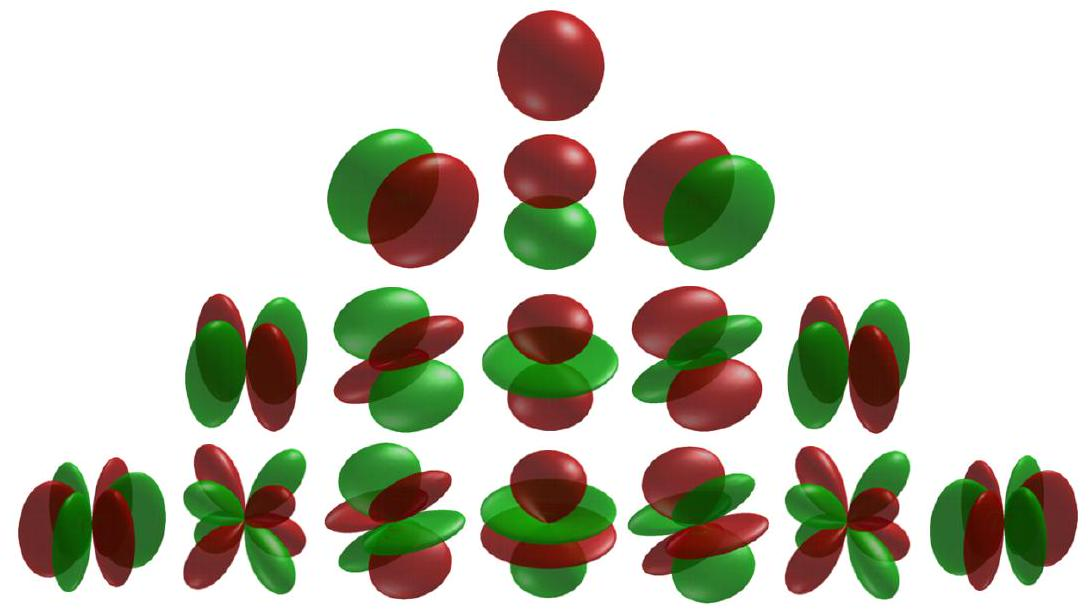
\includegraphics[scale=0.2]{2025_05_21_5017aafc65fbb33f9443g-12}
\end{center}

Figure 4.1: Die $s, p, d$ und $f$ Kugelfunktionen ( $l=0,1,2,3$, von oben nach unten) [Wikipedia]. Die benutzte radiale Abhängigkeit $R_{l m}(r)$ werden wir im Abschnitt ?? im Rahmen des Wasserstoffatoms diskutieren.

Beispiele

$$
\begin{aligned}
Y_{00} & =\frac{1}{\sqrt{4 \pi}} \\
Y_{11} & =-\left(\frac{3}{8 \pi}\right)^{\frac{1}{2}} \sin \vartheta e^{i \varphi} \\
Y_{10} & =\left(\frac{3}{4 \pi}\right)^{\frac{1}{2}} \cos \vartheta \\
Y_{1-1} & =\left(\frac{3}{8 \pi}\right)^{\frac{1}{2}} \sin \vartheta e^{-i \varphi}
\end{aligned}
$$

\section*{Nomenklatur}
Die Zustände mit $l=0,1,2,3$ werden auch als s-, p-, d- und f- Zustände bezeichnet. Die Bezeichnungen kommen aus der optischen Spektroskopkie. Historisch sind sie Abkürzungen für "scharfe","prinzipielle", "diffuse" und "feine" Linie.\\
definiert. Diese Beziehung gilt auch für negative $m$. Wegen

$$
P_{l}^{-m}(z)=(-1)^{m} \frac{(l-m)!}{(l+m)!} P_{l}^{m}(z)
$$

haben wir

$$
Y_{l m}(\varphi, \vartheta)=\left[\frac{(2 l+1)(l-m)!}{4 \pi(l+m)!}\right]^{\frac{1}{2}} P_{l}^{m}(\cos \vartheta) e^{i m \varphi}, \quad Y_{l-m}=(-1)^{m} Y_{l m}^{*}
$$

\subsubsection*{Eigenschaften der Kugelfunktionen}
Viele Formeln werden übersichtlicher, falls man die Variable $z=\cos \vartheta$ einführt:

$$
Y_{l m}(\varphi, \vartheta(z))=\frac{(-1)^{l}}{2^{l} l!} \sqrt{\frac{(2 l+1)(l+m)!}{4 \pi(l-m)!}}\left(1-z^{2}\right)^{-m / 2} \frac{d^{l-m}}{(d z)^{l-m}} \cdot\left(1-z^{2}\right)^{l} \cdot e^{i m \varphi}
$$

\section*{Legendre-Polynome}
Für $m=0$ definiert man

$$
Y_{l m=0}=\left(\frac{2 l+1}{4 \pi}\right)^{\frac{1}{2}} P_{l}(z) \quad P_{l}(z)=\frac{1}{2^{l} l!} \frac{d^{l}\left(z^{2}-1\right)^{l}}{d z^{l}}
$$

Die Funktionen $P_{l}(z)$ heißen Legendre-Polynome. Sie bilden ein vollständiges, orthogonales System im Intervall $[-1,+1]$.

\section*{Erzeugende Funktion}
Legendre-Polynome kann man auch durch ihre erzeugende Funktion definieren, d.h. als Entwicklungskoeffizienten einer geeigneten Taylorreihe. Es sei $|\vec{y}|<|\vec{x}|$, mit $s=|\vec{y}| /|\vec{x}|<$ 1:

$$
\begin{aligned}
|\vec{x}-\vec{y}|^{-1} & =\frac{1}{|\vec{x}|}\left(1-2 z s+s^{2}\right)^{-\frac{1}{2}} \\
& =\frac{1}{|\vec{x}|} \sum_{l=0}^{\infty} P_{l}(z) s^{l}
\end{aligned}
$$

Diese "Entwicklung nach Multipolen" ist u.A. in der Elektrodynamik von zentraler Bedeutung. ${ }^{4}$

\section*{Multipolentwicklung}
Die Funktionen $Y_{l m}(\vartheta, \varphi)$ bilden ein vollständiges System auf der Einheitskugel,

$$
0 \leq \vartheta \leq \pi, \quad 0 \leq \varphi \leq 2 \pi
$$

Ist $f(\varphi, \vartheta)$ eine quadratintegrable Funktion auf der Einheitskugel, $(f, f) \equiv \int d \Omega f^{*} f$, mit $(f, f)<\infty$, dann läßt sich $f(\varphi, \vartheta)$ nach Kugelfunktionen entwickeln:

$$
f(\varphi, \vartheta)=\sum_{l=0}^{\infty} \sum_{m=-l}^{m=+l} f_{l m} Y_{l m}(\vartheta, \varphi)
$$

\section*{Skalarprodukt}
Die Entwicklungskoeffizienten $f_{l m}$ sind durch das Skalarprodukt

$$
f_{l m}=\left(Y_{l m}, f\right)=\int d \Omega Y_{l m}^{*}(\vartheta, \varphi) f(\varphi, \vartheta)
$$

gegeben.

\footnotetext{${ }^{4}$ Z.B. für die Behandlung des Potentials $V(\vec{x})=\frac{1}{4 \pi \varepsilon_{0}} \int d^{3} y \frac{\rho(\vec{y})}{|\vec{x}-\vec{y}|}$. Hier is $\rho(\vec{y})$ die Ladungsdichte.
}\subsection*{Stern-Gerlach Experiment}
Der experimentelle Beweis für die "Quantelung" des Drehimpulses kann aus dem Stern-Gerlach-Versuch gewonnen werden. ${ }^{5}$

\section*{Bahndrehimpuls und magnetisches Dipolmoment}
Bewegt sich eine Punktladung $q$ eines Teilchens mit Masse $m_{0}$ auf einer geschlossenen Kurve $C$, so gehört zu dem Bahndrehimpuls $\vec{l}$ das magnetische Dipolmoment

$$
\vec{\mu}=\frac{q}{2 m_{0}} \vec{l}
$$

\section*{Teilchen in einem inhomogenen Magnetfeld}
Ferner wird auf einen punktförmigen magnetischen Dipol in einem inhomogenen Magnetfeld $\vec{B}(\vec{x})$ die Kraft

$$
\vec{K}(\vec{x})=\operatorname{grad}(\vec{\mu} \cdot \vec{B}(\vec{x}))
$$

ausgeübt.\\
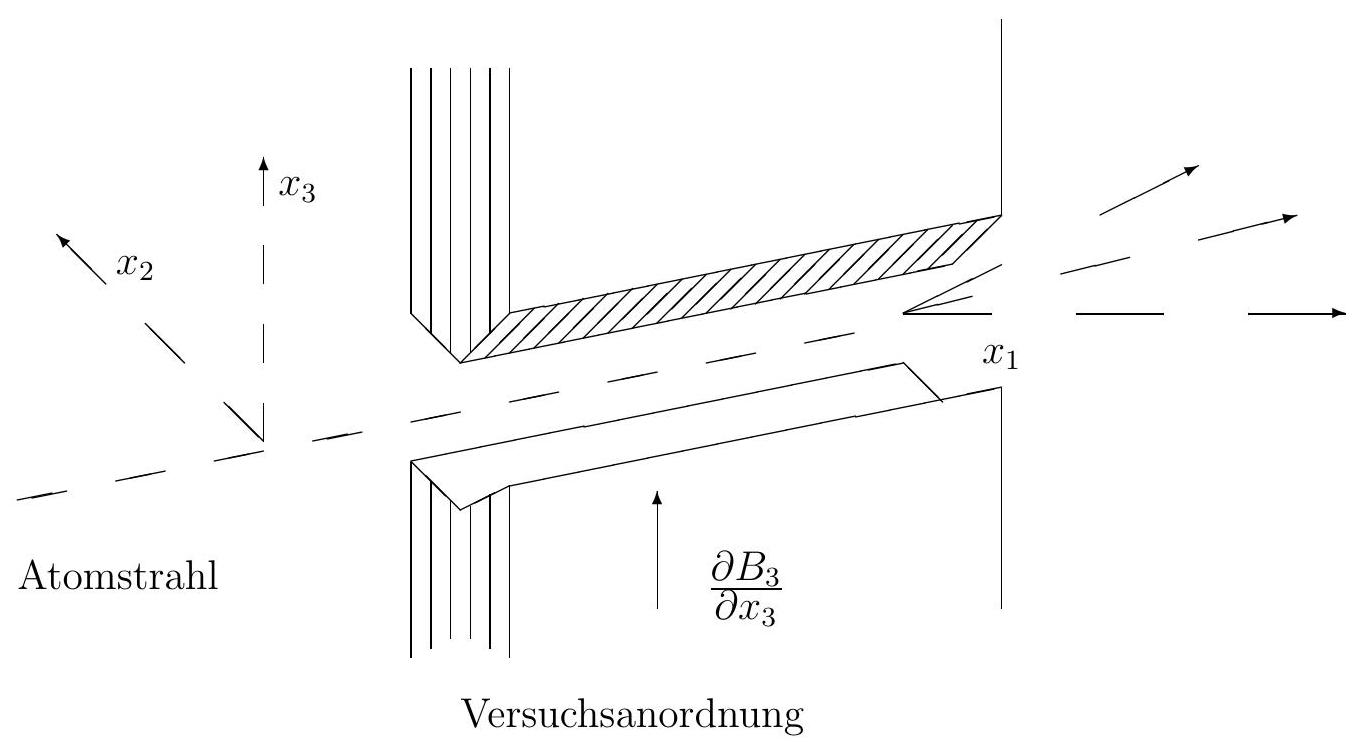
\includegraphics[scale=0.2, center]{2025_05_21_5017aafc65fbb33f9443g-14}

Von links (s. Skizze) werden Atome in der Ebene $x_{2}=0$ in ein inhomogenes Magnetfeld geschossen. Die Elektronen in den Atomen sollen bezüglich des Atomkernes den Drehimpuls (Bahndrehimpuls) $\vec{l}$ haben, und damit das magnetische Moment $\vec{\mu}=-\frac{e_{0}}{2 m_{e}} \vec{l}$, wobei

\footnotetext{${ }^{5}$ Dieser Versuch wurde 1922 von Otto Stern und Walter Gerlach im Physikalischen Institut der Universität Frankfurt durchgeführt.
}
$e_{0}>0$ die Elementarladung ist. Somit erfahren die Elektronen (und damit die Atome) in $x_{3}$-Richtung die Kraft
$$
K_{3}\left(x_{1}, x_{2}=0, x_{3}\right)=\frac{\partial}{\partial x_{3}}\left(\mu_{1} B_{1}+\mu_{2} B_{2}+\mu_{3} B_{3}\right)
$$

Zwischen den Magnetpolen ist $B_{1} \equiv 0$, d.h. $\partial_{3} B_{1}=0$. Ferner gilt $B_{2}\left(x_{2}=0\right)=0$ und damit $\partial_{3} B_{2}\left(x_{2}=0\right)=0$; also

$$
K_{3}\left(x_{1}, x_{2}=0, x_{3}\right)=\mu_{3} \partial_{3} B_{3}
$$

\section*{Aufspaltung des Bahndrehimpulses}
$\overline{\text { Quantenmechanisch gilt } l_{3} \rightarrow \hbar m \text {, mit } l}=0,1, \ldots$ und $\quad-l \leq m \leq l$. Also

$$
\mu_{3}=-\frac{e_{0} \hbar}{2 m_{e}} m, \quad-l \leq m \leq l
$$

Demnach wären also auch die magnetischen (Bahn-) Momente gequantelt. Enthält nun der einfallende Strahl Atome, bei denen äußere Elektronen relativ zum Kern den Bahndrehimpuls $\vec{l}$ haben, und sind (aufgrund der Präparierung) des Strahles etwa alle $x_{3}-$ Komponenten mit vergleichbaren Gewichten vertreten, so spaltet der Strahl aufgrund der Kraft $K_{3}$ in $2 l+1$ Komponenten räumlich auf (Nachweis z.B. durch Photoplatte).

Auf diese Weise kann man direkt nachweisen, daß die quantenmechanischen Bahndrehimpulse ganzzahlige Vielfache von $\hbar$ sind.

$$
\begin{array}{c|}
\hline \text { Die Größe } \mu_{B} \equiv \frac{e_{0} \hbar}{2 m_{e}} \text { heißt Bohr'sches Magneton. } \\
\mu_{B}=5,788382 \cdot 10^{-15} \mathrm{MeV} \text { gauss }^{-1}=5,788382 \cdot 10^{-11} \mathrm{MeV} T^{-1}
\end{array}
$$

\section*{Spin der Elektronen}
In vielen Fällen sind die $2 l+1$ Teilstrahlen nochmal gespalten (Feinstruktur). So hat man z.B. bei Alkali-Metallen für $l=0$ eine Aufspaltung in zwei Teilstrahlen. Dies rührt daher, daß die Elektronen einen Eigendrehimpuls oder Spin, $\vec{S}=\frac{\hbar}{2} \vec{\sigma}$, haben, und zu diesem das magnetische Moment

$$
\vec{\mu}_{e}=-\frac{e_{0}}{2 m_{e}} g \vec{S}, \quad g=2+2(1159,652193 \pm 0,000010) \times 10^{-6}
$$

gehört.






\pagebreak






\section{Rotationsinvariante Potentiale}

\subsection*{Schrödinger-Gleichung für rotationssymmetrische Potentiale}
\section*{Drehimpulserhaltung}
Für ein rotationssymmetrisches Potential $V(\vec{x})=V(|\vec{x}|)$ ist der Hamiltonian invariant unter Rotationen. Klassisch wie quantenmechanisch ist der Drehimpuls eine gute Quantenzahl. Es gilt

$$
\left[\mathbf{L}_{j}, \mathbf{H}\right]=0, \quad j=1,2,3, \quad \text { also auch } \quad\left[\overrightarrow{\mathbf{L}}^{2}, \mathbf{H}\right]=0
$$

Wie wir später noch sehen werden, ist ein Operator genau dann eine Erhaltungsgrösse, wenn er mit dem Hamiltonoperator vertauscht. Aus Abschnitt ?? wissen wir: Vertauschen zwei Operatoren, kann man sie gleichzeitig auf Diagonalform bringen. Dies bedeutet:

\begin{itemize}
  \item Man kann die Eigenfunktionen von
\end{itemize}

$$
\mathbf{H}=\frac{\overrightarrow{\mathbf{p}}^{2}}{2 m}+V(r)
$$

gleichzeitig als Eigenfunktionen zu $\overrightarrow{\mathbf{L}}^{2}$ und $\mathbf{L}_{3}$ wählen.\\
Beweis\\
Wir benutzen

$$
[A B, C]=A[B, C]+[A, C] B \quad[A B, C]=A B C-C A B
$$

um $\left[\mathbf{L}_{i}, \overrightarrow{\mathbf{p}}^{2}\right]=0$ nachzuvollziehen, sowie $\overrightarrow{\mathbf{p}}^{2}=p_{l} p_{l}$ :

$$
\begin{aligned}
\epsilon_{i j k}\left[x_{j} p_{k}, p_{l} p_{l}\right] & =\epsilon_{i j k}\left(x_{j}\left[p_{k}, p_{l} p_{l}\right]+\left[x_{j}, p_{l} p_{l}\right] p_{k}\right)=-\epsilon_{i j k}\left[p_{l} p_{l}, x_{j}\right] p_{k} \\
& =-\epsilon_{i j k}\left(p_{l}\left[p_{l}, x_{j}\right]+\left[p_{l}, x_{j}\right]\right) p_{k} \\
& =i \hbar \epsilon_{i l k}\left(p_{l}+p_{k}\right)
\end{aligned}
$$

Wegen $\epsilon_{i l k}=-\epsilon_{i k l}$ verschwindet der letzte Term.

In Bezug auf das Potential genügt die Bemerkung, dass die Komponenten des Drehimplusoperators mit jeder Operator-Funktion trivialerweise vertauschen, wenn diese nur von $r$ abhängt. Man betrachte z.B. $L_{3}=(\hbar / i) \partial_{\varphi}$.

\section*{Hamilton-Operator in Kugelkoordinaten}
Der Laplace-Operator lautet in sphärischen Koordinaten

$$
\begin{aligned}
\Delta & =\frac{1}{r^{2}} \frac{\partial}{\partial r}\left(r^{2} \frac{\partial}{\partial r}\right)+\frac{1}{r^{2} \sin ^{2} \vartheta}\left(\sin \vartheta \frac{\partial}{\partial \vartheta} \sin \vartheta \frac{\partial}{\partial \vartheta}+\frac{\partial^{2}}{\partial \varphi^{2}}\right) \\
& =\frac{1}{r} \frac{\partial^{2}}{\partial r^{2}} r-\frac{1}{r^{2} \hbar^{2}} \overrightarrow{\mathbf{L}}^{2}
\end{aligned}
$$

Die Herleitung ist länglich, ansonsten aber elementar. Der erste Term in der zweiten Gleichung ist lediglich eine alternative Darstellung, ${ }^{1}$ für den zweiten Term vergleiche Abschnitt ??. Der Ausgangspunkt unserer Überlegungen ist damit

$$
H=-\frac{\hbar^{2}}{2 r m_{0}} \frac{\partial^{2}}{\partial r^{2}} r+\frac{1}{2 m_{0} r^{2}} \overrightarrow{\mathbf{L}}^{2}+V(r)
$$

\section*{Entwicklung nach Kugelfunktionen}
Sei $u(\vec{x})$ eine Lösung der zeitunabhängigen Schrödinger-Gleichung. Wir entwickeln den Winkelanteil nach Kugelfunktionen $Y_{l m}$ :

$$
u(\vec{x})=\sum_{l=0}^{\infty} \sum_{m=-l}^{m=+l} R_{l m}(r) Y_{l m}(\vartheta, \varphi), \quad r=|\vec{x}|
$$

Damit wird die Schrödinger-Gleichung zu

$$
\begin{array}{r}
\sum_{l=0}^{\infty} \sum_{m=-l}^{m=+l}\left[-\frac{\hbar^{2}}{2 r m_{0}} \frac{\partial^{2}\left(r R_{l m}\right)}{\partial r^{2}}+\frac{\hbar^{2} l(l+1)}{2 m_{0} r^{2}} R_{l m}(r)+V(r) R_{l m}(r)\right] Y_{l m}(\vartheta, \varphi) \\
=E \sum_{l=0}^{\infty} \sum_{m=-l}^{m=+l} R_{l m}(r) Y_{l m}(\vartheta, \varphi)
\end{array}
$$

Multipliziert man diese Gleichung mit $Y_{l^{\prime} m^{\prime}}^{*}$ und integriert über $\vartheta$ und $\varphi$, so folgt wegen $\left(Y_{l_{1} m_{1}}, Y_{l_{2} m_{2}}\right)=\delta_{l_{1} l_{2}} \delta_{m_{1} m_{2}}$ für $R_{l m}(r)$ die Gleichung

$$
-\frac{\hbar^{2}}{2 r m_{0}} \frac{\partial^{2}\left(r R_{l m}\right)}{\partial r^{2}}+\left[\frac{\hbar^{2} l(l+1)}{2 m_{0} r^{2}}+V(r)\right] R_{l m}(r)=E R_{l m}(r)
$$

\section*{Zentrifugalpotential}
Im folgenden wird angenommen, daß das Zentrifugalpotential

$$
\frac{\hbar^{2} l(l+1)}{2 m r^{2}}
$$

\footnotetext{${ }^{1}(1 / r) \partial_{r}^{2} r=2 / r+\partial_{r}^{2}=\left(1 / r^{2}\right) \partial_{r}\left(r^{2} \partial_{r}\right)$.
}
für $l \neq 0$ und $r \rightarrow 0$ gegenüber $V(r)$ dominiert, d.h. dass
$$
\lim _{r \rightarrow 0}\left(r^{2} V(r)\right)=0
$$
gilt, wie es für das Coulomb-Potential der Fall ist. Anschaulich bedeutet dieses, daß auch quantenmechanisch das Teilchen nicht in den Ursprung "fallen" soll, die Wahrscheinlichkeitsdichte
$$
w(\vec{x})=u^{*}(\vec{x}) u(\vec{x})
$$
für $\vec{x} \rightarrow 0$ also endlich bleibt, d.h. $R_{l m}(r=0)$ soll endlich sein.

\section*{Verhalten für $r \rightarrow 0$}
Für $r \rightarrow 0$ kann man $E$ und $V(r)$ gegenüber $r^{-2}$ vernachlässigen:

$$
-\frac{d^{2}}{d r^{2}}\left(r R_{l m}(r)\right)-\frac{l(l+1)}{r^{2}} R_{l m}(r) \approx 0, \quad \text { für } \quad r \rightarrow 0 .
$$

Die Lösungen sind

$$
R_{l m}(r) \approx C r^{\nu}, \quad \nu(\nu+1)=l(l+1) ; \quad \quad \nu=l, \quad \text { oder } \quad \nu=-l-1
$$

Wenn $R_{l m}(r=0)<\infty$, kommt nur die reguläre Lösung $\nu=l$ in Frage

\subsection*{Die Bindungszustände des Wasserstoffatoms}
Es sei nun

$$
V(r)=-\frac{Z e_{0}^{2}}{4 \pi \varepsilon_{0} r}
$$

das Potential für ein Elektron mit Ladung $-e_{0}$ im Feld eines Kernes mit Ladung $Z e_{0}$. Mit $R_{l m}(r) \equiv R(r)$ wird die Schrödingergleichung für die radiale Wellenfunktion zu

$$
\left(\frac{d^{2}}{d r^{2}}+\frac{2}{r} \frac{d}{d r}\right) R+\frac{2 m_{0}}{\hbar^{2}}\left[E+\frac{Z e_{0}^{2}}{4 \pi \varepsilon_{0} r}-\frac{\hbar^{2} l(l+1)}{2 m_{0} r^{2}}\right] R(r)=0
$$

Gesucht werden quadratintegrierbare Lösungen mit $E<0$ (gebundene Zustände).

\section*{Dimensionslose Variablen}
Führt man die neuen Variablen

$$
\begin{aligned}
& \rho=\left(\frac{8 m_{0}|E|}{\hbar^{2}}\right)^{\frac{1}{2}} r, \lambda=Z \alpha\left(\frac{c^{2} m_{0}}{2|E|}\right)^{\frac{1}{2}} \\
& \alpha=\frac{e_{0}^{2}}{4 \pi \varepsilon_{0} \hbar c} \approx \frac{1}{137}: \text { Sommerfeldsche } \\
& \text { Feinstrukturkonstante }
\end{aligned}
$$

ein, so erhält man die radiale Schrödingergleichung

$$
\frac{d^{2} R}{d \rho^{2}}+\frac{2}{\rho} \frac{d R}{d \rho}+\left(\frac{\lambda}{\rho}-\frac{1}{4}-\frac{l(l+1)}{\rho^{2}}\right) R=0
$$

Die Kontrolparameter sind der Drehimplus $l(l+1)$ und $\lambda$.

\section*{Verhalten für $r \rightarrow \infty$}
Für große $\rho$ ergibt sich für $R \sim R_{\infty}(\rho)$ näherungsweise

$$
\frac{d^{2} R_{\infty}}{d \rho^{2}}-\frac{1}{4} R_{\infty}=0, \quad R_{\infty} \sim e^{ \pm \rho / 2}
$$

Als normierbare Lösung kommt nur $e^{-\rho / 2}$ in Frage.

\section*{Allgemeine Lösung}
Wir hatten bereits gezeigt, daß $R(\rho) \sim \rho^{l}$ für $\rho \rightarrow 0$ gilt. Daher betrachten wir nun den Ansatz

$$
R(\rho)=\rho^{l} e^{-\rho / 2} g(\rho)
$$

Hiermit finden wir für $g(\rho)$ die Gleichung

$$
\frac{d^{2} g(\rho)}{d \rho^{2}}+\left(\frac{2 l+2}{\rho}-1\right) \frac{d g}{d \rho}+\frac{\lambda-1-l}{\rho} g(\rho)=0
$$

\section*{Taylor-Entwicklung}
Wir entwickeln die Lösung in eine Taylorreihe in $\rho$,

$$
g(\rho)=\sum_{n=0}^{\infty} a_{n} \rho^{n}
$$

und setzen sie ein. Wir finden

$$
\sum_{n=0}^{\infty}\left[n(n-1) a_{n} \rho^{n-2}+\left(\frac{2 l+2}{\rho}-1\right) n a_{n} \rho^{n-1}+(\lambda-1-l) a_{n} \rho^{n-1}\right]=0
$$

bzw.

$$
\sum_{n=0}^{\infty}\left[(n+1)\left(n a_{n+1}+(2 l+2) a_{n+1}\right)+(\lambda-1-l-n) a_{n}\right] \rho^{n-1}=0
$$

Da diese Gleichung für alle $\rho$ gelten soll, müssen die Koeffizienten einzeln verschwinden:

$$
a_{n+1}=\frac{n+l+1-\lambda}{(n+1)(n+2 l+2)} a_{n}
$$

Bricht die Reihe nicht ab, so hätte man für große $n: a_{n+1} \sim \frac{1}{(n+1)} a_{n}$, d.h. $g(\rho)$ verhielte sich für große $\rho$ wie

$$
g(\rho) \sim e^{\rho}
$$

Dies würde jedoch zu einem nicht normierbaren $R(\rho)$ führen. Die Reihe muß für normierbare $R$ also abbrechen.

\section*{Hauptquantenzahl}
Es muß also ein $n=n_{r}$ geben, für welches $a_{n_{r}+1}=0$, d.h.

$$
\lambda=n_{r}+l+1, \quad n_{r} \geq 0
$$

\begin{center}
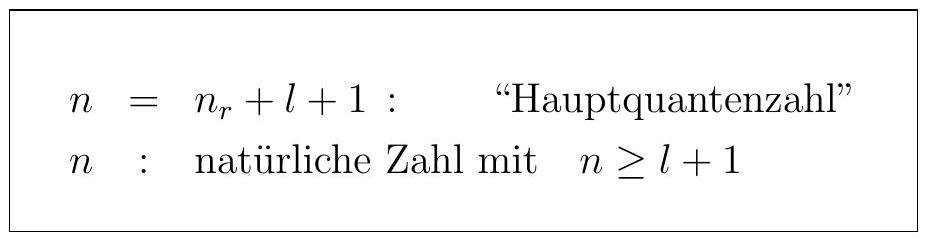
\includegraphics[scale=0.2]{2025_05_21_d5590f158a899e385c7cg-05}
\end{center}

Als muss $\lambda=Z \alpha \sqrt{\frac{c^{2} m_{0}}{2|E|}}$ eine ganze Zahl sein, $\lambda=n$. Hieraus folgt für die möglichen Energiewerte $E=E_{n}$ der gebundenen Zustände des Wasserstoffatoms:

$$
E_{n}=-\frac{1}{2} m_{0} c^{2} \frac{(Z \alpha)^{2}}{n^{2}} \quad \text { (Bohr'sche Formel) }
$$

\section*{Bahn-Quantenzahlen}
Die Abbruchbedingung

$$
a_{n_{r}+1}=0, \quad n-1=n_{r}+l
$$

hat für feste Hauptquantenzahl $n$ noch einen Freiheitsgrad,

$$
l=0,1, \ldots n-1
$$

Dieses sind die erlaubten Werte des Drehimpules.

\section*{Entartungsgrad}
Da zu $l$ schon $2 l+1$ Zustände mit verschiedenen $l_{3}$-Komponenten gehören, so ist der gesamte Entartungsgrad durch

$$
\sum_{l=0}^{n-1}(2 l+1)=n^{2}
$$

gegeben. Zu vorgegebenem $E_{n}$ gehören also $n^{2}$ verschiedene Bahndrehimpuls-Zustände. Berücksichtigt man außerdem, daß zu jedem Bahndrehimpuls-Zustand ( $l, m$ ) noch je 2 Spin-Zustände des Elektrons gehören, so bekommt man schließlich als Entartungsgrad von $E_{n}$ den Wert $d_{n}=2 n^{2}$. Dies ist die Dimension des zu $E_{n}$ gehörigen Unterraumes.

$$
d_{1}=2, \quad d_{2}=8, \quad d_{3}=18 \quad \text { etc. }
$$

Dieses Ergebnis ist für die Atomphysik wichtig.

\section*{Eigenfunktionen des Wasserstoffatoms}
Die Funktionen $g(\rho)$ sind Polynome vom Grad $n_{r}=n-l-1$, mit $n_{r}=0,1, \ldots$ Für gegebene $n$ und $l$ gilt die Rekursionsformel für die Koeffizienten $a_{\nu}$,

$$
a_{\nu+1}=\frac{\nu+l+1-n}{(\nu+1)(\nu+2 l+2)} a_{\nu} \quad \nu=0, \ldots n_{r}
$$

wobei $n_{r}=n-l-1$. Bei geeigneter Wahl von $a_{0}$ sind die Polynome identisch mit denn sogenannten zugeordneten Laguerre'schen Polynomen:

$$
\begin{aligned}
L_{n_{r}}^{\alpha}(\rho) & =\sum_{\nu=0}^{n_{r}}(-1)^{\nu}\binom{n_{r}+\alpha}{n_{r}-\nu} \frac{\rho^{\nu}}{\nu!} \\
& =\frac{1}{n_{r}!} e^{\rho} \rho^{-\alpha} \frac{d^{n_{r}}}{d \rho^{n_{r}}}\left(e^{-\rho} \rho^{n_{r}+\alpha}\right)
\end{aligned}
$$

Für $\alpha=0$ erhält man die Laguerre'schen Polynome. Für das Wasserstoffatom gilt $\alpha=$ $2 l+1$.

\section*{Beispiele}
Die radialen Eigenfunktionen $R_{n l m}(\rho) \equiv R_{n l}(\rho)$ des Wasserstoffatoms mit Energie $E_{n}$ sind

$$
R_{n l}(\rho)=C_{n l} e^{-\frac{1}{2} \rho} \rho^{l} L_{n-l-1}^{2 l+1}(\rho)
$$

wobei $C_{n l}$ der Normierungsfaktor ist. Setzt man

$$
a \equiv \frac{\hbar^{2} 4 \pi \varepsilon_{0}}{m_{e} e^{2}} \quad: \text { Bohr'scher Atomradius }
$$

so hat man z.B. (normiert)

$$
\begin{aligned}
& R_{10}(r)=2\left(\frac{Z}{a}\right)^{3 / 2} e^{-Z r / a} \\
& R_{20}(r)=2\left(\frac{Z}{2 a}\right)^{3 / 2}\left(1-\frac{Z r}{2 a}\right) e^{-Z r /(2 a)} \\
& R_{21}(r)=\frac{1}{\sqrt{3}}\left(\frac{Z}{2 a}\right)^{3 / 2} \frac{Z r}{a} e^{-Z r /(2 a)}
\end{aligned}
$$

\section*{Aufenthaltswahrscheinlichkeit}
Die Wahrscheinlichkeit, das Elektron in einer Kugelschale mit Radius $r$ und $r+\Delta r$ anzutreffen, ist durch

$$
w(\Delta r)=\int_{r}^{r+\Delta r} d r w_{n l}(r), \quad w_{n l}(r)=r^{2} R_{n l}^{2}(r)
$$

gegeben. Das Maximum der Aufenthaltswahrscheinlichkeit liegt für $w_{10}(r)=C_{10}^{2} r^{2} e^{-2 Z r} / a$ bei $r=a / Z$. Im allgemeinen hat $w_{n l}(r)$ genau $n-l$ Maxima.

Die Mittelwerte $<r^{k}>=\int_{0}^{\infty} d r r^{k} w_{n l}(r)$ lassen sich für $k= \pm 1$ einfach berechnen:

$$
<r>=\frac{a}{2 Z}\left[3 n^{2}-l(l+1)\right], \quad<r^{-1}>=\frac{Z}{a n^{2}}
$$

\subsubsection*{Korrekturen}
Die Bohr'sche Formel für die Energieniveaus des Elektrons im Wasserstoffatom stellt nur eine Näherung dar, zu der eine ganze Reihe von Korrekturen kommen (Feinstruktur, Hyperfeinstruktur etc).

\section*{Mitbewegung des Kernes}
Wir haben bisher so getan, als ob der Kern des Wasserstoffatoms unendlich schwer sei (und deshalb ruht). Tatsächlich haben Kern und Elektron die Masse

$$
c^{2} m_{p}=938 \mathrm{MeV}, \quad c^{2} m_{e}=0.51 \mathrm{MeV}
$$

und seine Mitbewegung macht sich bemerkbar.\\
Die Energie $\tilde{E}$ zweier Teilchen mit Koordinaten $\vec{x}_{i}=\left(x_{1}^{(i)}, x_{2}^{(i)}, x_{3}^{(i)}\right), i=1,2$, und wechselseitigem Potential $V\left(\vec{x}_{1}-\vec{x}_{2}\right)$ ist klassisch durch

$$
\tilde{E}=\frac{1}{2 m_{1}} \vec{p}_{1}^{2}+\frac{1}{2 m_{2}} \vec{p}_{2}^{2}+V\left(\vec{x}_{1}-\vec{x}_{2}\right)
$$

gegeben. Das Äquvalenzprinzip,

$$
\vec{p}_{1} \rightarrow \frac{\hbar}{i} \operatorname{grad}_{1}, \quad \vec{p}_{2} \rightarrow \frac{\hbar}{i} \operatorname{grad}_{2}, \quad \operatorname{grad}_{j}=\left(\frac{\partial}{\partial x_{1}^{(j)}}, \frac{\partial}{\partial x_{2}^{(j)}}, \frac{\partial}{\partial x_{3}^{(j)}}\right)
$$

führt zu der stationären Schrödinger-Gleichung für zwei Teilchen:

$$
\left(-\frac{\hbar^{2}}{2 m_{1}} \Delta_{1}-\frac{\hbar^{2}}{2 m_{2}} \Delta_{2}+V\left(\vec{x}_{1}-\vec{x}_{2}\right)\right) \tilde{u}\left(\vec{x}_{1}, \vec{x}_{2}\right)=\tilde{E} \tilde{u}\left(\vec{x}_{1}, \vec{x}_{2}\right)
$$

\section*{Schwerpunktskoordinaten}
Mittels Relativ- und Schwerpunktkoordinaten

$$
\begin{aligned}
\vec{x} & =\vec{x}_{1}-\vec{x}_{2}, & \vec{R}=\frac{\left(m_{1} \vec{x}_{1}+m_{2} \vec{x}_{2}\right)}{\left(m_{1}+m_{2}\right)} & \\
\vec{x}_{1} & =\vec{R}+\frac{\mu}{m_{1}} \vec{x}, & \vec{x}_{2}=\vec{R}-\frac{\mu}{m_{2}} \vec{x}, & \mu=\frac{m_{1} m_{2}}{m_{1}+m_{2}}
\end{aligned}
$$

wird die Kern-Elektron Schrödingergleichung zu

$$
\left(-\frac{\hbar^{2}}{2\left(m_{1}+m_{2}\right)} \Delta_{R}-\frac{\hbar^{2}}{2 \mu} \Delta_{x}+V(\vec{x})\right) \tilde{u}(\vec{x}, \vec{R})=\tilde{E} \tilde{u}(\vec{x}, \vec{R})
$$

die man auch herleiten kann, indem man das Äquivalenzprinzip direkt auf Relativ- und Schwerpunkts-Koordinaten anwendet. Hier is $m_{1}+m_{2}$ die Gesamtmasse und $\mu=m_{1} m_{2} /\left(m_{1}+\right.$ $m_{2}$ ) die Relativmasse, wie schon aus der Mechanik bekannt.

\section*{Seperation der Variablen}
Als Separation der Variablen nennt man Produkt-Ansätze für die Lösung von Differentialgleichungen, wie $\psi(\vec{x}, t)=u(\vec{x}) \exp (i E t / \hbar)$. Der analoge Ansatz für Relativ- und Schwerpunkts-Koordinaten ist

$$
\tilde{u}(\vec{x}, \vec{R})=u(\vec{x}) u(\vec{R}), \quad u(\vec{R})=e^{i \vec{K} \cdot \vec{R}}
$$

wobei wir davon Gebrauch gemacht haben, daß der der Gesamptimpuls $\vec{p}_{1}+\vec{p}_{2}$ erhalten ist, d.h. dass sich die Schwerpunktskoordinate frei bewegt (als ebene Welle). Die Schrödingergleichung für die Relativ-Koordinate ist damit

$$
\left(-\frac{\hbar^{2}}{2 \mu} \Delta_{x}+V(\vec{x})\right) u(\vec{x})=E u(\vec{x}), \quad E=\tilde{E}-\frac{\hbar^{2} \vec{K}^{2}}{2\left(m_{1}+m_{2}\right)}
$$

Dabei ist

$$
\begin{aligned}
\frac{\hbar^{2} \vec{K}^{2}}{2\left(m_{1}+m_{2}\right)} & : \text { kinetische Energie des Schwerpunktes } \\
E & : \text { Energie der Relativbewegung }
\end{aligned}
$$

Die Schrödinger-Gleichung für die Relativbewegung ist also die gleiche wie für die Bewegung in einem äußeren Potential $V(\vec{x})$. Man hat lediglich die Masse $m$ durch die reduzierte Masse $\mu=m_{1} m_{2} /\left(m_{1}+m_{2}\right)$ zu ersetzen.

\section*{Energieniveaus}
Die Energie-Niveaus des Wasserstoffatoms ist somit

$$
E_{n}=-\frac{1}{2} \mu c^{2} \frac{\alpha^{2}}{n^{2}}, \quad \mu=\frac{m_{e}}{1+m_{e} / m_{p}}
$$

Geht man vom Proton zum Deuteron über, so hat man $m_{p} \rightarrow m_{d} \approx 2 m_{p}$ und eine entsprechende Verschiebung der Energieniveaus des schwerer Wasserstoffs. Aufgrund dieses Effektes wurde das Deuteron entdeckt. Eine Reihe weiterer physikalischer Effekte führen zu Korrekturen der Bohr'schen Energieniveaus.

\begin{itemize}
  \item Das magnetischen Moment des Elektrons.
  \item Relativistischen Geschwindigkeit des Elektrons.
  \item Das magnetischen Moment des Kerns.
\end{itemize}

\subsection*{Radialsymmetrische Lösungen für $V(r)=0$}
Die Lösungen der freien Schrödinger-Gleichung lassen sich in verschiedenen Systemen von Basisfunktionen darstellen. Bisher haben wir dazu ebenen Wellen verwendet, die Eigenfunktionen des Impulsoperators.

Hier betrachten wir Lösungen der Form $R_{l m}(r) Y_{l m}(\vartheta, \varphi)$, welche bei Streuprozessen auftreten. Zunächst beschäftigen wir uns mit der Lösung für die radialen Wellenfunktionen, $R_{l m}(r)$. und schreiben kurz $R_{l m}(r) \equiv R_{l}(r)$. Für $V \equiv 0$ hat die radiale Schrödingergleichung die Form

$$
-\frac{\hbar^{2}}{2 m r} \frac{\partial^{2}\left(r R_{l}\right)}{\partial r^{2}}+\frac{\hbar^{2} l(l+1)}{2 m r^{2}} R_{l}(r)=E R_{l}(r)
$$

Da diese freie Teilchen beschreibt, sind die Energie-Eigenwerte kontinuierlich, aber positiv, $E \geq 0$.

\subsubsection*{Sphärische Bessel- und Neumann-Funktionen}
Es gibt verschiedene Wege, dimensionslose Variable für die radiale Schrödingergleichung einzuführen, eine Möglichkeit haben wir auf Seite 4 im Zusammenhang mit der Diskussion gebundener Zustände benutzt. Hier setzen wir

$$
\frac{2 m E}{\hbar^{2}}=k^{2}=|\vec{k}|^{2}, \quad \text { und } \quad \rho \equiv k r
$$

Damit erhalten wir

$$
\frac{d^{2} R_{l}}{d \rho^{2}}+\frac{2}{\rho} \frac{d R_{l}}{d \rho}-\frac{l(l+1)}{\rho^{2}} R_{l}+R_{l}=0
$$

Man beachte, daß die Energie $\hbar^{2} k^{2} /(2 m)$ nur via der Reskalierung des radialen Abstandes eingeht, via $\rho=k r$. Als Differentialgleichung 2. Ordnung hat diese Gleichung zwei unabhängige Lösungen, welche man auch "sphärischen Zylinderfunktionen" nennt.

\section*{Bessel-Funktion}
Die Lösungen der radialen Schrödinger-Gleichung stehen in einem engen Zusammenhang mit den Bessel-Funktionen $J_{\nu}(\rho)$ :

$$
\begin{aligned}
0 & =\frac{d^{2} J_{\nu}}{d \rho^{2}}+\frac{1}{\rho} \frac{d J_{\nu}}{d \rho}+\left(1-\frac{\nu^{2}}{\rho^{2}}\right) J_{\nu}(\rho) \\
J_{\nu}(\rho) & =\frac{\rho^{\nu}}{2^{\nu}} \sum_{k=0}^{\infty}(-1)^{k} \frac{\rho^{2 k}}{2^{2 k} k!\Gamma(\nu+k+1)}
\end{aligned}
$$

Diese werden überall da gebraucht, wo es um Lösungen der Laplace Gleichung in polaroder sphärischen Koordinaten geht. Dabei kann $\nu$ complex sein.

\section*{Sphärische Bessel-Funktion}
Wir betrachten nun die bei $\rho=0$ reguläre Lösung, die sphärische Bessel-Funktion $j_{\nu}(\rho)$ :

$$
j_{l}(\rho)=\left(\frac{\pi}{2 \rho}\right)^{\frac{1}{2}} J_{l+\frac{1}{2}}(\rho), \quad j_{l}(\rho)=(-\rho)^{l}\left(\frac{1}{\rho} \frac{d}{d \rho}\right)^{l}\left(\frac{\sin \rho}{\rho}\right)
$$

Aus der zweiten Darstellung folgt

$$
j_{0}(\rho)=\frac{\sin \rho}{\rho}, \quad j_{1}(\rho)=\frac{\sin \rho}{\rho^{2}}-\frac{\cos \rho}{\rho}
$$

Man kann durch vollständige Induktion verifizieren, dass die $j_{l}(\rho)$ Lösungen der radialen Schrödingergleichung sind. D.h. man beweist zunächst den Fall $l=0$ und schliesst dann aus der Richtigkeit für $l$ auf die Richtigkeit für $l+1$.

\section*{Sphärische Neumann-Funktionen}
Wir betrachten nun die bei $\rho=0$ singuläre Lösung, die sphärische Neumann-Funktionen $n_{l}(\rho)$ :

$$
n_{l}(\rho)=(-1)^{l+1}\left(\frac{\pi}{2 \rho}\right)^{\frac{1}{2}} J_{-l-\frac{1}{2}}(\rho), \quad n_{l}(\rho)=-(-\rho)^{l}\left(\frac{1}{\rho} \frac{d}{d \rho}\right)^{l}\left(\frac{\cos \rho}{\rho}\right)
$$

Mit

$$
n_{0}(\rho)=-\frac{\cos \rho}{\rho}, \quad n_{1}(\rho)=-\frac{\cos \rho}{\rho^{2}}-\frac{\sin \rho}{\rho}
$$

\section*{Grenzwertverhalten}
Für $\rho \rightarrow 0$ gilt

$$
\begin{aligned}
& j_{l}(\rho) \approx \frac{\rho^{l}}{(2 l+1)!!} \quad(2 l+1)!!\equiv 1 \cdot 3 \cdot 5 \cdots(2 l+1) \\
& n_{l}(\rho) \approx \frac{-(2 l-1)!!}{\rho^{l+1}}
\end{aligned}
$$

Für $\rho \rightarrow \infty$ gilt andererseits

$$
j_{l}(\rho) \sim \frac{1}{\rho} \sin \left(\rho-\frac{l \pi}{2}\right), \quad n_{l}(\rho) \sim-\frac{1}{\rho} \cos \left(\rho-\frac{l \pi}{2}\right)
$$

\subsubsection*{Entwicklung von ebenen Wellen nach Legendre-Polynomen}
Ebene Wellen,

$$
e^{i \vec{k} \cdot \vec{x}}=e^{i k r \cos \vartheta}=e^{i \rho z}, \quad \vartheta=\angle(\vec{k}, \vec{x}), \quad \rho=k r, \quad z \cos \vartheta,
$$

sind reguläre Lösungen von $\left(\Delta+k^{2}\right) u(\vec{x})=0$, sie lassen sich daher ebenfalls nach Kugelfunktionen und sphärischen Bessel-Funktionen $j_{l}(\rho)$ entwickeln.

Eine ebene Welle hängt von der Energie $\hbar^{2} k^{2} /(2 m)$ nur via der Reskalierung des radialen Abstandes $\rho=k r \mathrm{ab}$, sie ist zudem rotations-invariant um die Ausbreitungsrichtung $\vec{k}=(0,0, k)$, und damit unabhängig vom Polarwinkel $\varphi$. In der Entwicklung nach Kugelfunktionen $Y_{l m}(\varphi, \vartheta)$ treten daher nur die Terme $m=0$ auf, und damit nur die Legendre Polynome

$$
P_{l}(z)=\left(\frac{4 \pi}{2 l+1}\right)^{1 / 2} Y_{l 0}, \quad z=\cos \vartheta
$$

also

$$
e^{i \rho z}=\sum_{l=0}^{\infty} c_{l} j_{l}(\rho) P_{l}(z)
$$

Der radiale Anteil ist durch die sphärische Besselfunktion $j_{l}(\rho)$ gegeben, da diese die für $\rho \rightarrow 0$ regulär sind.

\section*{Entwicklungskoeffizienten}
Es bleiben die Entwicklungskoeffizienten $c_{l}$ mit Hilfe der Orthogonalitätsrelationen

$$
\int_{-1}^{+1} d z P_{l_{1}}(z) P_{l_{2}}(z)=\frac{2 \delta_{l_{1} l_{2}}}{\left(2 l_{1}+1\right)}, \quad c_{l} j_{l}(\rho)=\frac{2 l+1}{2} \int_{-1}^{+1} d z P_{l}(z) e^{i \rho z}
$$

für Legendre-Polynome zu bestimmen. Wenn wir $z^{n}$ nach $P_{l}(z)$ entwicklen, so tragen nur Terme $l \leq n$ bei. Andererseits ist $P_{l}(z)$ orthogonal zu allen $P_{n}(z)$ mit $n \neq l$, daher gilt

$$
\int_{-1}^{+1} d z z^{n} P_{l}(z)=\left\{\begin{array}{cc}
0 & \text { für } n<l \\
\frac{2 l!}{(2 l+1)!!} & \text { für } n=l
\end{array}\right.
$$

Für $e^{i \rho z}=\sum_{n=0}^{\infty}(i \rho z)^{n} /(n!)$ finden wir daher

$$
\int_{-1}^{+1} d z P_{l}(z) e^{i \rho z}=\frac{2}{(2 l+1)!!}(i \rho)^{l}+O\left(\rho^{l+1}\right)
$$

Wir können jetzt den Grenzwert $\rho \rightarrow 0$ betrachten. Mit $j_{l}(\rho) \rightarrow \rho^{l} /(2 l+1)$ !! erhalten

$$
c_{l} j_{l}(\rho) \approx c_{l} \frac{\rho^{l}}{(2 l+1)!!} \approx \frac{(2 l+1)}{2} \frac{2(i \rho)^{l}}{(2 l+1)!!}+\ldots \quad \text { (höhere Potenzen in } \rho \text { ) }
$$

Ein Koeffizientenvergleich führt via

$$
c_{l}=(2 l+1) i^{l}
$$

zu dem zentralen Ergebnis

$$
e^{i \vec{k} \cdot \vec{x}}=e^{i k r \cos \vartheta}=\sum_{l=0}^{\infty}(2 l+1) i^{l} j_{l}(k r) P_{l}(\cos \vartheta)
$$

\section*{Physikalische Interpretation}
Das asymptotischen Verhaltens der spährischen Bessel Funktion $j_{l}(\rho)$ für große $\rho$ ist

$$
j_{l}(\rho) \sim \frac{1}{\rho} \sin \left(\rho-\frac{l \pi}{2}\right)=-\frac{1}{2 i k r}\left[e^{-i\left(k r-\frac{1}{2} l \pi\right)}-e^{i\left(k r-\frac{1}{2} l \pi\right)}\right]
$$

mit

$$
\begin{aligned}
& \frac{1}{r} e^{-i(\omega t+k r)} \quad: \text { ein-laufende Kugelwelle } \\
& \frac{1}{r} e^{-i(\omega t-k r)} \quad: \text { aus-laufende Kugelwelle }
\end{aligned}
$$

wobei $\omega=\hbar k^{2} /(2 m)$. Um ein- und auslaufende Wellen zu unterscheiden betrachtet man den Ort konstanter Phase, $\omega t+k r=0$. Die sphärische Besselfunktion $j_{l}(\rho)$ ist also für große Abstände ( $k r \gg 1$ ) eine Superposition von ein- und auslaufenden Kugelwellen. Der Drehimpuls $l$ geht nur via der Phasenverschiebung $l \pi / 2$ ein.

Beweis\\
Man bemerke, dass $\sin (\rho-l \pi / 2)$ je nach Quantenzahl $\pm \sin (\rho)$ entspricht ( $l$ gerade), bzw. $\pm \cos (\rho)$ (l ungerade). ${ }^{2}$ Das ist in Einklang mit

$$
j_{l}(\rho)=(-\rho)^{l}\left(\frac{1}{\rho} \frac{d}{d \rho}\right)^{l}\left(\frac{\sin \rho}{\rho}\right)=(-\rho)^{l}\left(\frac{1}{\rho} \frac{d}{d \rho}\right)^{l-1}\left(\frac{\cos \rho}{\rho}-\frac{\sin \rho}{\rho^{2}},\right)
$$

wobei der zweite Term für grosse $\rho$ verschindet.

\subsection*{Elastische Potentialstreuung}
\section*{Voraussetzung}
Für die Formulierung der Streutheorie brauchen wir die Annahme, dass sich die ungebundenen Lösungen der Schrödinger-Gleichung im Unendlichen wie ebene Wellen verhalten. Dazu muss das Potential $V(r)$ schnell genug für $r \rightarrow \infty$ abfallen, man kann zeigen, daß dies für

$$
\lim _{r \rightarrow \infty}(r V(r))=0,
$$

der Fall ist. Wir behandeln hier nicht die Streuung am Coulomb-Potential, die eine gesonderte Behandlung braucht.

\footnotetext{${ }^{2}$ Gemäß dem Ableitungs-Zyklus sin $\rightarrow \cos \rightarrow(-\sin ) \rightarrow(-\cos ) \rightarrow \sin$.
}
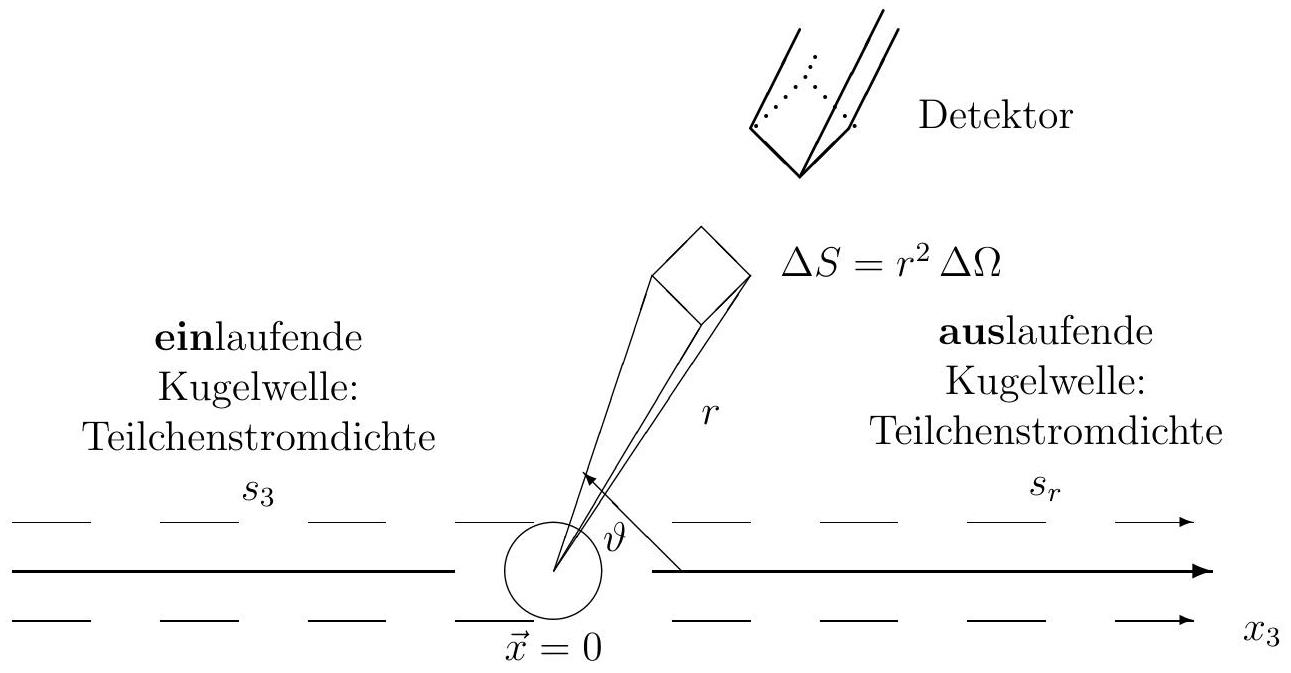
\includegraphics[scale=0.2, center]{2025_05_21_d5590f158a899e385c7cg-13}

\section*{Experimenteller Aufbau}
Längs der $x_{3}$-Achse fallen Teilchen der Stromdichte $s_{3}$ ein ${ }^{3}$ die am Streuzentrum in $\vec{x}=$ 0 (Relativkoordinate) in das Raumwinkelelement $\Delta \Omega$ mit radialer Teilchenstromdichte $s_{r}(r, \vartheta, \varphi)$ gestreut werden. Durch ein Flächenelement $\Delta S$ im Abstand $r$ treten dann pro Zeiteinheit $s_{r} \Delta S$ Teilchen.

Raumwinkelelement : $\Delta \Omega=\sin \vartheta \Delta \vartheta \Delta \varphi$

$$
\text { Fäschenelement : } \Delta S=r^{2} \Delta \Omega
$$

Stromdichte einfallender Teilchen : $s_{3}$\\
radiale Teilchenstromdichte : $\quad s_{r}(r, \vartheta, \varphi)=\vec{s} \cdot \vec{e}_{r}$

\section*{Wirkungsquerschnitt}
Der differentielle Wirkungsquerschnitt für die Streuung in das Raumwinkelelement $\Delta \Omega$ ist durch

$$
\begin{aligned}
\Delta \sigma(\vartheta, \varphi) & =\frac{s_{r} r^{2} \Delta \Omega}{s_{3}} \\
\frac{d \sigma}{d \Omega}(\vartheta, \varphi) & =\frac{s_{r}(r, \vartheta, \varphi) r^{2}}{s_{3}}
\end{aligned}
$$

definiert. Die Größe $d \sigma / d \Omega$ ist i.a. eine Funktion der Energie $E=\hbar^{2} k^{2} /(2 \mu)$, wobei $\mu$ die reduzierte Masse ist. Für rotationssymmetrische $V(\vec{x})$ hängt $d \sigma / d \Omega$ nicht von $\varphi \mathrm{ab}$.

\section*{Streuamplituden}
Sei $u(\vec{x})$ die Lösung der stationären Schrödinger-Gleichung zum Potential $V(r)$. Diese Lösung soll für große $r=|\vec{x}|$ aus einlaufender ebener Welle und auslaufender Kugelwelle

\footnotetext{${ }^{3}$ Vergleich den Abschnitt ?? zur Kontinuitätsgleichung.
}
bestehen,
$$
u(\vec{x}) \sim e^{i \vec{k} \cdot \vec{x}}+f(k, \vartheta) \frac{e^{i k r}}{r}, \quad \vec{k}=(0,0, k)
$$
mit $f(k, \vartheta)=0$ für $V(r)=0$. Die Größe $f(k, \vartheta)$ heißt Streuamplitude. Aus der Kontinuitätsgleichung folgt
$$
s_{3}=\hbar k_{3} / \mu, \quad s_{r}=\hbar k|f(k, \vartheta)|^{2} /\left(\mu r^{2}\right)
$$
und somit
$$
\frac{d \sigma(k, \vartheta)}{d \Omega}=\frac{s_{r} r^{2}}{s_{3}}=|f(k, \vartheta)|^{2}
$$
da $k_{3}=k$.

\section*{Entwicklung nach Partialwellen}
Die Partialwellen-Entwicklung ebener Wellen (siehe Abschnitt 5.3.2) reduziert sich für große $r$ zu

$$
\begin{aligned}
e^{i \vec{k} \cdot \vec{x}} & =\sum_{l=0}^{\infty}(2 l+1) i^{l} j_{l}(k r) P_{l}(\cos \vartheta) \\
& \sim-\frac{1}{2 i k} \sum_{l=0}^{\infty}(2 l+1) i^{l}\left(\frac{e^{-i\left(k r-\frac{1}{2} l \pi\right)}}{r}-\frac{e^{i\left(k r-\frac{1}{2} l \pi\right)}}{r}\right) P_{l}(\cos \vartheta)
\end{aligned}
$$

Diese ebene Welle entspricht dem Fall $V(r)=0$. Falls nun $V(r) \neq 0$, so wird lediglich die Amplitude/Phase der auslaufende Kugelwelle modifiziert. Wir machen den Ansatz

$$
u(\vec{x}) \approx-\frac{1}{2 i k} \sum_{l=0}^{\infty}(2 l+1) i^{l}\left(\frac{e^{-i\left(k r-\frac{1}{2} l \pi\right)}}{r}-S_{l}(k) \frac{e^{i\left(k r-\frac{1}{2} l \pi\right)}}{r}\right) P_{l}(\cos \vartheta)
$$

\section*{Streuphasen}
Bei einer rein elastischen Streuung können keine Teilchen verlorengehen, es werden also nur die Phasen, aber nicht jedoch die Intensitäten der auslaufenden Kugelwelle geändert werden. Also gilt $\left|S_{l}(k)\right|=1$ (bei inelastischer Streuung hat man $\left|S_{l}(k)\right|<1$ ), d.h.

$$
S_{l}(k)=e^{2 i \delta_{l}(k)}
$$

$$
\delta_{l}(k) \quad \text { : zur l-ten "Partialwelle" gehörige Streuphase. }
$$

Der Radialanteil $R_{l}(r)$ der Wellenfunktion verhält sich für große $r$ also asymptotisch wie

$$
R_{l}(r) \sim-\left(\frac{e^{-i\left(k r-\frac{1}{2} l \pi\right)}}{2 i k r}-e^{2 i \delta_{l}(k)} \frac{e^{i\left(k r-\frac{1}{2} l \pi\right)}}{2 i k r}\right)=e^{i \delta_{l}(k)} \frac{\sin \left(k r-\frac{1}{2} l \pi+\delta_{l}(k)\right)}{k r}
$$

\section*{Partialwellenentwicklung für Streuamplituden}
$\overline{\text { Mit } S_{l}=\left(S_{l}-1\right)+1 \text { läßt sich das obige } u(\vec{x}) \text { auch als }}$

$$
u(\vec{x}) \sim e^{i \vec{k} \cdot \vec{x}}+\left[\sum_{l=0}^{\infty}(2 l+1) i^{l} \frac{S_{l}(k)-1}{2 i k} P_{l}(\cos \vartheta) \frac{e^{i\left(k r-\frac{1}{2} l \pi\right)}}{r}\right]
$$

schreiben. Benutzen wir

$$
e^{-\frac{i}{2} l \pi}=i^{-l}, \quad u(\vec{x}) \sim e^{i \vec{k} \cdot \vec{x}}+f(k, \vartheta) \frac{e^{i k r}}{r}
$$

so erhält man für große $r$ mit

$$
f(k, \vartheta)=\sum_{l=0}^{\infty}(2 l+1) \frac{e^{2 i \delta_{l}(k)}-1}{2 i k} P_{l}(\cos \vartheta)
$$

Partialwellenentwicklung für die Streuamplituden $f(k, \vartheta)$.

\section*{Totaler Wirkungsquerschnitt}
Integrieren wir den differentiellen Wirkungsquerschnitt über die Einheitskugel, so erhalten wir den totalen elastischen Wirkungsquerschnitt $\sigma_{e l}(k)$ :

$$
\sigma_{e l}(k)=\int d \Omega|f(k, \vartheta)|^{2}
$$

Wegen der Orthogonalität der $P_{l}(\cos \vartheta)$ und da $\left(e^{2 i \delta_{l}}-1\right) / 2 i=e^{i \delta_{l}} \sin \delta_{l}$, folgt

$$
\sigma_{e l}(k)=\frac{4 \pi}{k^{2}} \sum_{l=0}^{\infty}(2 l+1) \sin ^{2} \delta_{l}(k)
$$

Die Streuphasen $\delta_{l}(k)$ sind bei vorgegebenem Potential aus dem asymptotischen Verhalten der Partialwellen $R_{l}(k r)$ zu bestimmen. Als Beispiel werden wir weiter unten den 3dimensionalen Potentialtopf diskutieren.

\section*{Optisches Theorem}
Für den Imagninätteil $\Im m f(k, \vartheta)$ der Streuamplitude gilt

$$
\Im m f(k, \vartheta=0)=\frac{1}{k} \sum_{l=0}^{\infty}(2 l+1) \sin ^{2} \delta_{l}(k)
$$

da $\Im m\left(e^{i \delta_{l}} \sin \delta_{l}\right)=\sin ^{2} \delta_{l}(k)$ und $P_{l}(1)=1$, und somit

$$
\Im m f(k, \vartheta=0)=\frac{k}{4 \pi} \sigma_{e l}(k)
$$

Dieser Zusammenhang wird das Optisches Theorem genannt. Der Verlust an einfallender Intensität $\left(\sigma_{e l}\right)$ entsteht durch "kohärente" (elastische) Interferenz.

\subsection*{3-dimensionaler Potentialtopf}
Wir betrachten als Beispiel den 3-dimensionalen, rotations-symmetrischen Potentialtopf,

\begin{center}
\begin{tabular}{rlrlrl}
$V(r)$ & $=-V_{0}$ &  & für &  & $r<a$, \\
$V(r)$ & $=0$ &  & für &  & $V_{0}>0$ \\
 &  &  &  &  &  \\
\hline
\end{tabular}
\end{center}

Analog zum endlich tiefen Potentialtopf in einer Dimension (siehe Abschnitt ??), definieren wir

$$
\begin{array}{rlr}
q & =\frac{1}{\hbar} \sqrt{2 \mu\left(V_{0}+E\right)} & \\
\kappa & =\frac{1}{\hbar} \sqrt{-2 \mu E}, & \text { für } E<0 \\
k & =\frac{1}{\hbar} \sqrt{2 \mu E} \quad \text { für } E>0
\end{array}
$$

Wobei $E<0 / E>0$ gebundenen-/Streu-Zuständen entspricht. Wir berachten zuerst $E<0$.

\subsubsection*{Gebundene Zustände}
Für $E<0$ genügt $R_{l}(r)$ den Gleichungen

$$
\begin{array}{ll}
\frac{d^{2} R_{l}}{d r^{2}}+\frac{2}{r} \frac{d R_{l}}{d r}-\frac{l(l+1)}{r^{2}} R_{l}+q^{2} R_{l}=0, & r<a \\
\frac{d^{2} R_{l}}{d r^{2}}+\frac{2}{r} \frac{d R_{l}}{d r}-\frac{l(l+1)}{r^{2}} R_{l}-\kappa^{2} R_{l}=0, & r>a
\end{array}
$$

Für grosse $r$ folgt aus der zweiten Gleichung $R_{l}^{\prime \prime}=\kappa^{2} R_{l}$, also $R_{l} \sim \exp (-\kappa r)$.

\section*{Innerer Zustand}
Für $r<a$ kommt nur die bei $r=0$ reguläre Lösung in Frage, also die sphärische Bessel Funktion

$$
R_{l}(r)=A j_{l}(\rho), \quad r<a
$$

mit $\rho=q r$.

\section*{Äusserer Zustand}
Für $r>a$ muss die Lösung wie $\exp (-\kappa \rho)$ exponentiel abfallen. Welche der sphärischen Funktionen tut das?

Die Bestimmungsgleichungen für $R_{l}$ unterscheiden sich in den Termen $q^{2} R_{l}$, bzw $-\kappa^{2} R_{l}$, mit $q, \kappa \geq 0$. Für die Transformation auf die Normalform führt das zu $\rho=q r$ und $\rho=i \kappa r$, jeweils für die Argumente der entsprechenden sphärichen Funktionen. Die sphärischen Hankel-Funktionen,

$$
h_{l}^{(1)}(\rho) \equiv j_{l}(\rho)+i n_{l}(\rho)
$$

verhalten sich asymptotisch, also für $r \rightarrow \infty$, wie

$$
h_{l}^{(1)}(\rho) \sim \frac{\sin (\rho-l \pi / 2)}{\rho}-\frac{i}{\rho} \cos (\rho-l \pi / 2)=\frac{1}{i \rho} e^{i\left(\rho-\frac{1}{2} l \pi\right)} .
$$

Für $r>a$ erhält daher

$$
R_{l}(r)=B h_{l}^{(1)}(i \kappa r), \quad-\frac{\hbar^{2} \kappa^{2}}{2 \mu}=E=\frac{\hbar^{2} q^{2}}{2 \mu}-V_{0}
$$

wobei wir $\rho=i \kappa r$ eingesetzt haben.

\section*{Randbedingungen}
Die zulässigen Energiewerte $E$ ergeben sich aus den Anschlussbedingungen bei $r= \pm a$,

$$
\begin{aligned}
A j_{l}(a q) & =B h_{l}^{(1)}(i a \kappa) \\
\left.A \frac{d}{d r} j_{l}(r q)\right|_{r=a} & =\left.B \frac{d}{d r} h_{l}^{(1)}(i r \kappa)\right|_{r=a}
\end{aligned}
$$

aus denen die transzendenten Bestimmungsgleichungen

$$
\frac{\frac{d}{d r} j_{l}(r q)}{j_{l}(r q)}=\frac{\frac{d}{d r} h_{l}^{(1)}(i r \kappa)}{h_{l}^{(1)}(i r \kappa)} \quad r=a, \quad l=0,1, \ldots
$$

folgen. Diese Gleichungen sind i.a. nur numerisch zu lösen.

\section*{Tiefer Potentialtopf}
Für einen tiefen Topf, d.h. für $q a \gg 1$ ( da $q \sim \sqrt{V_{0}+E}$ ), kann man auf der linken Seite die asymptotischen Formen für $j_{l}(r q)$ benutzen:

$$
\begin{aligned}
j_{l}(r q) & \sim \frac{1}{r q} \sin \left(r q-\frac{l \pi}{2}\right) \\
\frac{d j_{l}(r q)}{d r} & \sim-\frac{1}{r^{2} q} \sin \left(r q-\frac{l \pi}{2}\right)+\frac{1}{r} \cos \left(r q-\frac{l \pi}{2}\right)
\end{aligned}
$$

Einsetzen ergibt

$$
-\frac{1}{a}+q \cot \left(q a-\frac{l \pi}{2}\right)=\frac{\left.\frac{d}{d r} h_{l}^{(1)}(i r \kappa)\right|_{r=a}}{h_{l}^{(1)}(i a \kappa)}
$$

Da die Hankel-Funktionen die Lösungen für $r>a$ sind (wo $V(x)=0$ ), hängt die rechte Seite nicht von $V_{0} \mathrm{ab}$. Die linke Seite hängt via $q$ jedoch von $V_{0}$ ab, also muß für $|E| \ll V_{0}$ (hieraus folgt: grosses $q$ ) der Kotangens auf der linken Seite asymptotisch klein sein,

$$
\cot \left(q a-\frac{l \pi}{2}\right) \approx 0, \quad q a-\frac{l \pi}{2}=\left(m+\frac{1}{2}\right) \pi, \quad m=0,1, \ldots
$$

oder

$$
a q \approx\left(m+\frac{1}{2}\right) \pi+l \frac{\pi}{2}, \quad m=0,1 \ldots
$$

Via $q=\sqrt{2 \mu\left(V_{0}+E\right)} / \hbar$ ergeben sich hieraus für kleine $|E|$ die Energieeigenwerte der gebundenen Zustände.

\subsubsection*{Streuzustände}
Für Streuzustände is die Energie positive, $E>0$. Das bedeutet für $r>a$ :

$$
R_{l}(r)=B j_{l}(k r)+C n_{l}(k r)
$$

für $r<a$ gilt wie vorher $R_{l}(r)=A j_{l}(q r)$ (wobei jetzt $E>0$ ). Die Stetigkeitsbedingungen bei $r=a$ sind

$$
\frac{\left.\frac{d}{d r} j_{l}(q r)\right|_{r=a}}{j_{l}(q a)}=\frac{\left.\frac{d}{d r}\left(B j_{l}(k r)+C n_{l}(k r)\right)\right|_{r=a}}{B j_{l}(k a)+C n_{l}(k a)}
$$

Damit ist $C / B$ bestimmt.\\
Verhalten für $r \rightarrow \infty$\\
Das asymptotische Verhalten der sphärischen Bessel- und von Neumann-Funktionen für große $r$ bedeutet für die den Radialteil der Lösung

$$
R_{l}(r) \sim \frac{1}{k r}\left[B \sin \left(k r-\frac{l \pi}{2}\right)-C \cos \left(k r-\frac{l \pi}{2}\right)\right]
$$

Mit $\sin (\alpha+\beta)=\sin \alpha \cos \beta+\sin \beta \cos \alpha$ gilt

$$
\begin{aligned}
R_{l}(r) & \sim \frac{e^{i \delta_{l}}}{k r} \sin \left(k r-\frac{l \pi}{2}+\delta_{l}\right) \\
& =\frac{e^{i \delta_{l}}}{k r}\left[\sin \left(k r-\frac{l \pi}{2}\right) \cos \left(\delta_{l}\right)+\cos \left(k r-\frac{l \pi}{2}\right) \sin \left(\delta_{l}\right)\right]
\end{aligned}
$$

für den allgemeinen Ausdruck des Radialanteils durch die Streuphasen $\delta_{l}$ (siehe Abschnit 5.4). Der Vergleich ergibt

$$
B=e^{i \delta_{l}} \cos \left(\delta_{l}\right), \quad C=-e^{i \delta_{l}} \sin \left(\delta_{l}\right), \quad \tan \delta_{l}(k)=-\frac{C}{B}
$$

Wir eliminieren $C / B$ und erhalten schlussendlich die Streuphasen:

$$
\tan \delta_{l}(k)=\frac{\frac{d}{d r} j_{l}(k r) j_{l}(q a)-\frac{d}{d r} j_{l}(q r) j_{l}(k a)}{\frac{d}{d r} n_{l}(k r) j_{l}(q a)-\frac{d}{d r} j_{l}(q r) n_{l}(k a)}
$$

wobei die Ableitungen an der Stelle $r=a$ auszuwerten sind.

\subsubsection*{Grenzfälle}
Niederenergie-Streuung $k a \ll l$\\
$\overline{\text { Der Impuls }} \hbar k=\sqrt{2 \mu E}$ sei klein, und damit auch die kinetische Energie ausserhalb\\
des Potentialtopf. Dieser kann beliebig tief sein, also auch $q=\sqrt{2 \mu\left(V_{0}+E\right)} / \hbar$. Damit können wir aus dem Ausdruck für $\tan \delta_{l}(k)$ nach kleinen $k r$ entwickeln, nicht aber nach $q r$. Wir verwenden

$$
j_{l}(\rho) \approx \frac{\rho^{l}}{(2 l+1)!!}, \quad n_{l}(\rho) \approx-\frac{(2 l-1)!!}{\rho^{l+1}}, \quad \text { für } \quad \rho \rightarrow 0
$$

mit $(2 l+1)!!=(2 l+1) \cdot(2 l-1)!!$, und erhalten

$$
\tan \delta_{l}(k) \approx \frac{2 l+1}{[(2 l+1)!!]^{2}}(k a)^{2 l+1} \frac{l j_{l}(q a)-a \frac{d}{d r} j_{l}(q r)}{(l+1) j_{l}(q a)+a \frac{d}{d r} j_{l}(q r)}
$$

wobei die Ableitung wieder bei $r=a$ zu nehmen sind. Der Factor $(k a)^{2 l+1}$ setzt sich aus $\rho^{l} \cdot \rho^{l+1}$ zusammen.

\section*{Schwellen-Verhalten}
Das Schwellen-Verhalten

$$
\tan \delta_{l}(k) \approx c_{l} k^{2 l+1} \quad \text { für } \quad k \rightarrow 0
$$

gilt nicht nur für den Potentialtopf, sondern für alle Potentiale, deren Streuverhalten für $k \rightarrow 0$ bzw. $r \rightarrow 0$ durch das Zentrifugalpotential dominiert wird.

Schreibt man für den totalen elastischen Wirkungsquerschnitt, siehe Abschnitt 5.4,

$$
\sigma_{e l}(k)=\sum_{l=0}^{\infty} \sigma_{l}(k), \quad \sigma_{l}(k)=\frac{4 \pi(2 l+1)}{k^{2}} \sin ^{2} \delta_{l}(k)
$$

so hat man für $k \rightarrow 0$, da $\sin \alpha \approx \tan \alpha$ für $\alpha \rightarrow 0$,

$$
\begin{aligned}
\sigma_{l}(k) & =\frac{4 \pi(2 l+1)}{k^{2}}\left|C_{l}\right|^{2} k^{4 l+2}, \quad \text { d.h. } \\
\lim _{k \rightarrow 0} \sigma_{l}(k) & = \begin{cases}\text { const. } \neq 0 & \text { für } \quad l=0 \\
0 & \text { für } \quad l \neq 0\end{cases}
\end{aligned}
$$

\section*{Unitärer Limes}
Für gewisse Energien $E_{R}=\hbar^{2} k_{R}^{2} /(2 \mu)$ verschwindet der Nenner in der obigen Formel für $\tan \delta_{l}(k)$. Man hat dann

$$
\tan \delta_{l}\left(k_{R}\right)= \pm \infty, \quad \delta_{l}\left(k_{R}\right)=\left(m+\frac{1}{2}\right) \pi, \quad m \text { ganze Zahl. }
$$

Mit $\sin ^{2}[(n+1 / 2) \pi]=1$ werden die partiellen Streuquerschnitte $\sigma_{l}(k)$ für $k=k_{R}$ maximal,

$$
\sigma_{l}\left(k_{R}\right)=\frac{4 \pi(2 l+1)}{k_{R}^{2}}=\frac{4 \pi \hbar^{2}(2 l+1)}{2 \mu E_{R}}
$$

der unitärer Limes.

\section*{Resonanzstreuung}
Diese Phänomen läßt sich als eine Resonanzerscheinung interpretieren. Der Einfachheit halber sei

$$
\frac{a}{\hbar} \sqrt{2 \mu\left(V_{0}+E\right)}=q a \gg 1 \gg k a=\frac{a}{\hbar} \sqrt{2 \mu+E}
$$

(tiefer Topf und Niederenergiestreuung). Bei dieser Approximation kann man die oben entwickele Näherungsformel für $\tan \delta_{l}$ für Niederenergiestreuung benutzen. An der Resonanz, d.h. für $k=k_{R}$ und $q=q_{R}$, gilt die Bedingung

$$
(l+1) j_{l}\left(q_{R} a\right)+\left.a \frac{d}{d r} j_{l}\left(q_{R} r\right)\right|_{r=a}=0
$$

Wegen der Annahme $\rho=q_{R} a \gg 1$ können wir für die sphärische Besselfunktion den genäherten Ausdruck $j_{l}(\rho) \sim \sin (\rho-l \pi / 2) / \rho$ für große Argumente benutzen (siehe Abschnitt 5.3.2),

$$
\begin{aligned}
0 & =\frac{l+1}{a q_{R}} \sin \left(q_{R} a-\frac{l \pi}{2}\right)+\cos \left(q_{R} a-\frac{l \pi}{2}\right)-\frac{1}{q_{R}^{2}} \sin \left(q_{R} a-\frac{l \pi}{2}\right) \\
& \approx \cos \left(q_{R} a-\frac{l \pi}{2}\right)
\end{aligned}
$$

Hieraus folgt

$$
a q_{R}=m \pi+\frac{1}{2}(l+1) \pi, \quad m \text { ganz. }
$$

Dies sind aber gerade die gleichen Bedingungen wie für die diskreten gebundenen Zustände aus Abschnitt 5.5.1. Im Unterschied zu den (echten) gebundenen Zuständen ist hier jedoch $E_{R}>0$. Es handelt sich um ausgezeichnete diskrete Energieniveaus, die z.B. bei der Streuung angeregt werden, ähnlich wie bei erzwungenen Schwingungen in der Mechanik und Elektrodynamik:

Bei bestimmten Frequenzen $\omega_{R}=E_{R} / \hbar$ der einfallenden Teilchen werden die Eigenschwingungen des streuenden Systems angeregt.

\section*{'Instabile' Bindungszutände}
Resonanz-Niveaus $E_{R}$ lassen sich in gewisser Hinsicht als instabile Bindungszustände interpretieren:\\
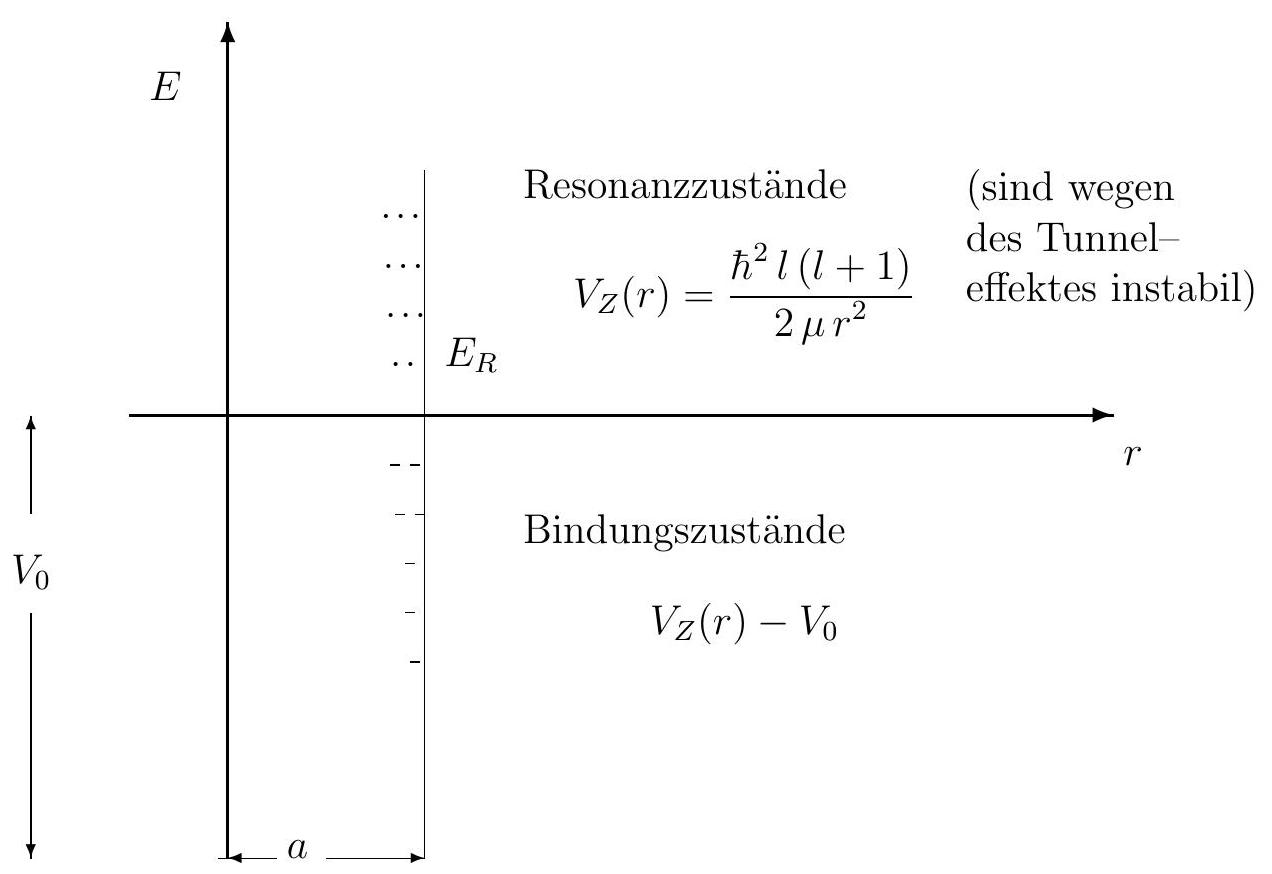
\includegraphics[scale=0.2, center]{2025_05_21_d5590f158a899e385c7cg-21}

\section*{Breit-Wigner Formel}
In der Nähe der Resonanz kann man näherungsweise

$$
\tan \delta_{l}=\gamma_{l} \frac{(k a)^{2 l+1}}{E-E_{R}}, \quad \gamma_{l}=\text { const }
$$

setzen: Schwellenverhalten für den Zähler, Taylor-Entwicklung um die Nullstelle im Nenner. Für den Wirkungsquerschnitt $\sigma_{l}$ der Partialwelle $l$ ergibt sich daraus

$$
\begin{aligned}
\sigma_{l}(E) & =\frac{4 \pi(2 l+1)}{k^{2}} \sin ^{2} \delta_{l}=\frac{4 \pi(2 l+1)}{k^{2}} \frac{\tan ^{2} \delta_{l}}{1+\tan ^{2} \delta_{l}} \\
& =\frac{4 \pi(2 l+1)}{k^{2}} \frac{\left(\gamma_{l}(k a)^{2 l+1}\right)^{2}}{\left(E-E_{R}\right)^{2}+\left(\gamma_{l}(k a)^{2 l+1}\right)^{2}}
\end{aligned}
$$

Dies ist die Breit-Wigner-Formel für den Wirkungsquerschnitt in der Umgebung der Resonanzenergie $E_{R}$.

\section*{Resonanzbreite}
Die entsprechende Amplitude der Partialwelle ist

$$
f_{l}(k)=\frac{1}{2 i k}\left(e^{2 i \delta_{l}(k)}-1\right)=\frac{1}{2 i k}\left(\frac{1+i \tan \delta_{l}}{1-i \tan \delta_{l}}-1\right)=\frac{1}{k} \frac{\tan \delta_{l}}{1-i \tan \delta_{l}}
$$

wobei wir $\exp (2 x)=\exp (x) / \exp (-x)$ verwendet haben. Man erhält

$$
f_{l}(k)=\frac{1}{k} \frac{\gamma_{l}(k a)^{2 l+1}}{E-E_{R}-i \gamma_{l}(k a)^{2 l+1}}
$$

Die Größe

$$
\Gamma_{l}=2 \gamma_{l}(k a)^{2 l+1}
$$

bezeichnet man als die Breite der Resonanz, da $\sigma_{l}\left(E_{R} \pm \frac{1}{2} \Gamma_{l}\right)=\frac{1}{2} \sigma_{l}\left(E_{R}\right)$.\\
Die Resonanzstreuung spielt eine zentral Rolle in der Atom-, Kern- und Elementarteilchenphysik. In ihrer allgemeinen Form gelten die hier hergeleiteten Formeln für viele Potentiale.\\
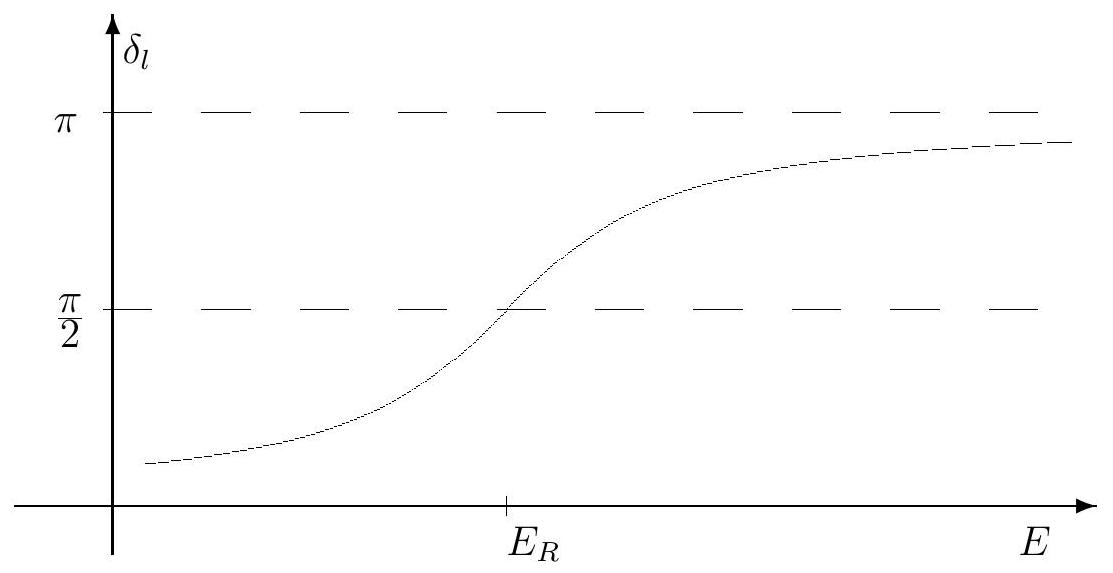
\includegraphics[scale=0.2, center]{2025_05_21_d5590f158a899e385c7cg-22}








\pagebreak



\section*{Der Spin der Elektronen}
\subsection*{Quantenmechanische Beschreibung}
Die Existenz des Spins bedeutet, daß Elektronen, außer der Ortskoordinate $\vec{x}$, oder der Impulskoordinate $\vec{p}$, einen weiteren Freiheitsgrad besitzen: Spin nach "oben" und Spin nach "unten", jeweils bezüglich einer vorgegebenen Richtung (Quantisierungsachse, z.B. die $x_{3}$-Richtung). Und dieses obwohl Elektronen Punktteilchen sind.

\section*{Spinore}
Man verdoppelt die Wellenfunktion $\psi(\vec{x}, t)$ zu einem Spinor $\tilde{\psi}(\vec{x}, t)$,

$$
\psi(\vec{x}, t) \rightarrow \quad \tilde{\psi}(\vec{x}, t)=\binom{\psi_{+}(\vec{x}, t)}{\psi_{-}(\vec{x}, t)}
$$

wobei $\psi_{+}(\vec{x}, t)$ ein Elektron mit Spin "oben" und $\psi_{-}(\vec{x}, t)$ ein Elektron mit Spin "unten" beschreibt.

\section*{Pauli-Matrizen}
Der Spin-Operator $\overrightarrow{\mathbf{S}}$ ist nach Anbschnitt ?? durch die Pauli-Matrizen $\sigma_{i}$ gegeben,

$$
\begin{aligned}
\overrightarrow{\mathbf{S}} & =\frac{\hbar}{2}\left(\sigma_{1}, \sigma_{2}, \sigma_{3}\right) \\
\sigma_{1} & =\left(\begin{array}{cc}
0 & 1 \\
1 & 0
\end{array}\right), \quad \sigma_{2}=\left(\begin{array}{cc}
0 & -i \\
i & 0
\end{array}\right), \quad \sigma_{3}=\left(\begin{array}{cc}
1 & 0 \\
0 & -1
\end{array}\right)
\end{aligned}
$$

Bis auf den Faktor $\hbar / 2$ folgen die Pauli Matrizen den Kommuationsrelationen von Drehimpulsoperatoren,

$$
\left[\sigma_{k}, \sigma_{l}\right]=2 i \epsilon_{k l m} \sigma_{m}, \quad \sigma_{j}^{2}=1, \quad j=1,2,3
$$

\section*{Basiswahl}
Bezeichen wir mit $\tilde{\psi}_{ \pm}$die Zustände mit Spin rauf/runter,

$$
\tilde{\psi}_{+}=\binom{1}{0}, \quad \tilde{\psi}_{-}=\binom{0}{1}
$$

so gilt erwartungsgemäß:

$$
\mathbf{S}_{3} \tilde{\psi}_{+}=\frac{\hbar}{2}\left(\begin{array}{cc}
1 & 0 \\
0 & -1
\end{array}\right)\binom{1}{0}=\frac{\hbar}{2}\binom{1}{0}, \quad \mathbf{S}_{3} \tilde{\psi}_{-}=-\frac{\hbar}{2}\binom{0}{1}
$$

Für festes $\vec{x}$ und $t$ spannen $\tilde{\psi}_{+}$und $\tilde{\psi}_{-}$einen 2-dimionalen Vektorraum auf, dessen Elemente als Spinoren bezeichnet werden.

\section*{Wellenfunktionen}
Ein allgemeines Element des Vektorraums hat komplexen Koeffizienten $c_{+}$und $c_{-}$, die orts- und zeitabhängig sind:

$$
\tilde{\psi}(\vec{x}, t)=c_{+}(\vec{x}, t) \tilde{\psi}_{+}+c_{-}(\vec{x}, t) \tilde{\psi}_{-}=\binom{c_{+}(\vec{x}, t)}{c_{-}(\vec{x}, t)}
$$

Die Entwicklungskoeffizienten $c_{ \pm}(\vec{x}, t)$ entsprechen also Wellenfunktionen $\psi_{ \pm}(\vec{x}, t)$, von denen es pro Elektron nun zwei gibt. Die Norm von $\tilde{\psi}(\vec{x}, t)$ ist durch

$$
(\tilde{\psi}, \tilde{\psi})=\left|c_{+}\right|^{2}+\left|c_{-}\right|^{2}
$$

gegeben. Wegen der physikalischen Interpretation muss $(\tilde{\psi}, \tilde{\psi})=1$ sein. $\left|c_{ \pm}\right|^{2}$ ist damit die Wahrscheinlichkeit dafür, daß ein Elektron im Zustand $\psi$ den Spin parallel/antiparallel zur $x_{3}$-Achse ausgerichtet hat, mit $\left|c_{+}\right|^{2}+\left|c_{-}\right|^{2}=1$.

\section*{Erwartungswerte}
Im folgenden wird die Ortsabhängigkeit von $\tilde{\psi}$ ignoriert und zunächst nur Spineigenschaften betrachtet. Für die Erwartungswerte $\left\langle\mathbf{S}_{j}\right\rangle$ der Komponenten $\mathbf{S}_{j}$ im Zustand $\tilde{\psi}$ ergibt sich

$$
<\mathbf{S}_{1}>=\frac{\hbar}{2}\left(c_{+}^{*}, c_{-}^{*}\right)\left(\begin{array}{ll}
0 & 1 \\
1 & 0
\end{array}\right)\binom{c_{+}}{c_{-}}=\frac{\hbar}{2}\left(c_{+}^{*} c_{-}+c_{-}^{*} c_{+}\right),
$$

und analog

$$
\begin{aligned}
& <\mathbf{S}_{2}>=-\frac{i \hbar}{2}\left(c_{+}^{*} c_{-}-c_{-}^{*} c_{+}\right) \\
& <\mathbf{S}_{3}>=\frac{\hbar}{2}\left(\left|c_{+}\right|^{2}-\left|c_{-}\right|^{2}\right)
\end{aligned}
$$

Als Observable sind die Erwartungswerte reel.

\subsection*{Drehungen von Spins}
Im Abschnitt ?? wurde gezeigt, daß Wellenfunktionen via

$$
\psi(R \vec{x})=e^{-i \overrightarrow{\mathbf{L}} \cdot \vec{\varphi} / \hbar} \psi(\vec{x})
$$

gedreht werden. Dieses gilt für ganzzahligen Drehimpuls $j=0,1,2 \ldots$ Für $j=1 / 2$ ist der Drehimpulsoperatoren $\vec{L}$ durch den Spin-Operator $\vec{S}$ zu ersetzen,

$$
R \tilde{\psi}=e^{-i \overrightarrow{\mathbf{S}} \cdot \vec{\varphi} / \hbar} \tilde{\psi}
$$

wobei $\tilde{\psi}$ ein Spinor ist.

\section*{Drehung um die z-Achse}
Als Beispiel betrachten wir eine Drehung um die 3-Achse, d.h. $\vec{\varphi}=(0,0, \varphi)$ :

$$
\begin{aligned}
e^{-i \mathbf{S}_{3} \varphi / \hbar} & =\sum_{n=0}^{\infty} \frac{(-i \varphi / 2)^{n}}{n!}\left(\begin{array}{cc}
1 & 0 \\
0 & -1
\end{array}\right)^{n} \\
& =\sum_{l=0}^{\infty} \frac{(-i \varphi / 2)^{(2 l)}}{(2 l)!}\left(\begin{array}{ll}
1 & 0 \\
0 & 1
\end{array}\right)+\sum_{l=0}^{\infty} \frac{(-i \varphi / 2)^{(2 l+1)}}{(2 l+1)!}\left(\begin{array}{cc}
1 & 0 \\
0 & -1
\end{array}\right) \\
& =\cos (\varphi / 2)\left(\begin{array}{ll}
1 & 0 \\
0 & 1
\end{array}\right)-i \sin (\varphi / 2)\left(\begin{array}{cc}
1 & 0 \\
0 & -1
\end{array}\right)=\left(\begin{array}{cc}
e^{-i \varphi / 2} & 0 \\
0 & e^{i \varphi / 2}
\end{array}\right)
\end{aligned}
$$

Spin nach oben und unten erhalten also entgegengesetzte Phasen.

$$
\text { Bei einer Drehung um } 2 \pi \text { erhalten Spinoren die Phase }(-1) \text {. }
$$

Um einen Spin in den Ausgangszustand überzuführen bedarf es also einer Drehung um $4 \pi$.

\subsection*{Das magnetische Moment des Elektrons}
\section*{Gyromagnetischer Faktor}
Ein Elektron mit Spin ist ein rotierendes (geladenes) Teilchen. Aus der Elektrodynamik wissen wir, daß ein Ringstrom mit Drehimpuls $\vec{L}=\vec{S}$ ein magnetisches Moment der Grösse

$$
\begin{aligned}
\vec{\mu} & =-\frac{e_{0} g}{2 m_{e}} \overrightarrow{\mathbf{S}} & & \text { mit } \\
g & \approx 2 & & \text { (in guter Näherung) }
\end{aligned}
$$

erzeugt. Der $g$-Faktor heißt gyromagnetischer Faktor. Für klassische Ringströme gilt $g=1$, siehe auch Abschnitt ??.

\section*{Elektron im Magnetfeld}
In einem äußeren Feld $\vec{B}$ hat ein klassisches magnetisches Moment $\vec{\mu}$ die Energie $-\vec{\mu} \cdot \vec{B}$. Nach dem Korrespondenzprinzip führt dies zum Hamilton-Operator

$$
\mathbf{H}=\frac{e_{0} g \hbar}{4 m_{e}} \vec{\sigma} \cdot \vec{B}
$$

Für einen zeitabhängigen Spinor $\tilde{\psi}(t)=\binom{c_{+}(\vec{x}, t)}{c_{-}(\vec{x}, t)}$ erhalten wir die zeithabhängige Schrödinger-Gleichung

$$
i \hbar \frac{d}{d t} \tilde{\psi}(t)=\frac{e_{0} g \hbar}{4 m_{e}}(\vec{\sigma} \cdot \vec{B}) \tilde{\psi}(t)
$$

\section*{Lamor-Frequenz}
Wir betrachten ein konstantes Magnetfeld $\vec{B}=\left(0,0, B_{0}\right)$ und lösen die SchrödingerGleichung mittels des Ansatzes $\tilde{\psi}(t)=e^{-i \omega t}\binom{c_{+}}{c_{-}}$, mit $c_{ \pm}=$const., also

$$
\hbar \omega\binom{c_{+}}{c_{-}}=\frac{e g \hbar B_{0}}{4 m_{e}}\left(\begin{array}{cc}
1 & 0 \\
0 & -1
\end{array}\right)\binom{c_{+}}{c_{-}} .
$$

Die beiden Eigenfrequenzen $\omega_{ \pm}$sind

$$
\omega_{+}=\frac{e_{0} g B_{0}}{4 m_{e}} \equiv \omega_{L} \quad \text { und } \quad \omega_{-}=-\omega_{L}
$$

mit Eigenvektoren sind $(1,0)$ und $(0,1)$. Hier is $\omega_{L}$ die Lamor-Frequenz. ${ }^{1}$ Für einen allgemeinen Anfangszustand $\tilde{\psi}(t=0)=(a, b)$ findet man daher

$$
\tilde{\psi}(t)=\binom{a e^{-i \omega_{L} t}}{b e^{i \omega_{L} t}}, \quad \omega_{L}=\frac{e_{0} g B}{4 m_{e}}, \quad|a|^{2}+|b|^{2}=1
$$

\section*{Präzession}
Als Beispiel betrachten wir einen Anfangszustand, in welchem der Spin entlang der 1Achse ausgericht ist, also senkrecht zum angelegten Magnetfeld.

Als Erstes müssen wir den Eigenvektor $(a, b)$ zu $\mathbf{S}_{1}$ (und zum Eigenwert $\hbar / 2$ ) finden:

$$
\frac{1}{2} \hbar\left(\begin{array}{ll}
0 & 1 \\
1 & 0
\end{array}\right)\binom{a}{b}=\frac{1}{2} \hbar\binom{a}{b}, \quad\binom{a}{b}=\frac{1}{\sqrt{2}}\binom{1}{1} .
$$

\footnotetext{${ }^{1}$ Die hier definierte Larmor-Frequenze gilt für Spin-1/2. Klassisch benutzt man $q g B /(2 m)$. Unter Einberechnung der $g$-Faktoren erhält man sehr ähnliche Werte.
}Wir berechnen nun den Zeit-abhängigen Erwartungswert,

$$
\begin{aligned}
\left(\tilde{\psi}(t), \mathbf{S}_{1} \tilde{\psi}(t)\right) & =<\mathbf{S}_{1}>(t) \\
& =\frac{\hbar}{2} \frac{1}{\sqrt{2}}\left(e^{i \omega_{L} t}, e^{-i \omega_{L} t}\right)\left(\begin{array}{cc}
0 & 1 \\
1 & 0
\end{array}\right)\binom{e^{-i \omega_{L} t}}{e^{i \omega_{L} t}} \frac{1}{\sqrt{2}} \\
& =\frac{\hbar}{2} \cos 2 \omega_{L} t
\end{aligned}
$$

Analog ergibt sich

$$
\begin{aligned}
<\mathbf{S}_{1}>(t) & =\frac{\hbar}{2} \cos 2 \omega_{L} t \\
<\mathbf{S}_{2}>(t) & =\frac{\hbar}{2} \sin 2 \omega_{L} t \\
<\mathbf{S}_{3}>(t) & =0
\end{aligned}
$$

d.h. der Spin "präzediert" mit der doppelten Lamor-Frequenz um die Richtung von $\vec{B}$.

\subsection*{Paramagnetische Resonanz}
Der $g$-Faktor in der Beziehung

$$
\vec{\mu}=\frac{q g}{2 m} \overrightarrow{\mathbf{S}}, \quad \overrightarrow{\mathbf{S}}=\frac{1}{2} \hbar \vec{\sigma}, \quad q: \text { Ladung }
$$

ist im Festkörper keine universelle Konstante, sondern hängt von der chemischen Umgebung ab (via der Spin-Bahn Kopplung, siehe Abschnitt ??). Eine Methode die Größe des $g$-Faktors experimentell zu bestimmen ist die paramagnetische Resonanz.

\section*{RF-Felder}
Analog zu der Induktion von atomaren Übergängen zwischen verschiedenen Niveaus durch Einstrahlen von Licht, kann man Übergänge zwischen den beiden Energieniveaus $\pm \hbar \omega_{L}=$ $\hbar g|q| B_{0} /(4 m)$ eines Spins in einem konstanten Magnetfeld $B_{0}$ induzieren. Dafür benötigt man ein zusätzlich oszillierendes Magnetfeld $B$, typischerweise im Radiofrequenz (RF) Bereich.

Es sei also

$$
\vec{B}=\left(B \cos \omega t, B \sin \omega t, B_{0}\right)
$$

Mit

$$
\vec{\sigma} \cdot \vec{B}=\left(\begin{array}{cc}
B_{0}, & B(\cos \omega t-i \sin \omega t) \\
B(\cos \omega t+i \sin \omega t), & -B_{0}
\end{array}\right)
$$

lautet die Schrödinger-Gleichung (mit $q=-e_{0}$ )

$$
i \hbar \frac{d \tilde{\psi}}{d t}=\frac{\hbar q g}{4 m}\left(\begin{array}{cc}
B_{0}, & B e^{-i \omega t} \\
B e^{i \omega t}, & -B_{0}
\end{array}\right) \tilde{\psi}(t)
$$

\section*{Variation der Konstanten}
Die Energie ist nicht erhalten, da $\mathbf{H}=\mathbf{H}(t)=\hbar \omega_{g} \vec{\sigma} \cdot \vec{B}(t)$ explizit von der Zeit abhängt, analog zu erzwungenen Schwingungen in der Mechanik.

Der Ansatz (Variation der Konstanten)

$$
\tilde{\psi}(t)=\binom{a(t) e^{-i \omega_{L} t}}{b(t) e^{i \omega_{L} t}}, \quad \frac{d \tilde{\psi}}{d t}=\binom{\left(\dot{a}-i \omega_{L} a\right) e^{-i \omega_{L} t}}{\left(\dot{b}+i \omega_{L} b\right) e^{i \omega_{L} t}}
$$

führt zu den Gleichungen

$$
\begin{aligned}
\dot{a} & =-i \omega_{g} e^{i\left(2 \omega_{L}-\omega\right) t} b(t) \\
\dot{b} & =-i \omega_{g} e^{-i\left(2 \omega_{L}-\omega\right) t} a(t) \\
\omega_{g} & =\left(g e_{0} B\right) /(4 m)
\end{aligned}
$$

Differenzieren der 1. Gleichung nach $t$ und Einsetzen der zweiten ergibt

$$
\ddot{a}-i\left(2 \omega_{L}-\omega\right) \dot{a}+\omega_{g}^{2} a=0
$$

Der Ansatz $a(t)=A e^{i \lambda t}$ führt zu einer quadratischen Gleichung für $\lambda$, mit den Lösungen

$$
\lambda_{1,2}=\omega_{L}-\frac{1}{2} \omega \pm \sqrt{\left(\omega_{L}-\frac{1}{2} \omega\right)^{2}+\omega_{g}^{2}}
$$

Die Bewegung des Systems, d.h. des Spinors $\tilde{\psi}(t)$ wird also durch die äussere Frequenz $\omega$ moduliert.

\section*{Induzierte Übergänge}
Wir preparieren das System zur Zeit $t=0$ in den Spin-oben Zustand: $a(0)=1$ und $b(0)=0$, was auch $\dot{a}(0)=0$ bedeutet. Für allg. Zeiten gilt

$$
\begin{aligned}
a(t) & =\left[\cos (\widehat{\omega} t)-i \frac{\omega_{L}-\omega / 2}{\widehat{\omega}} \sin \widehat{\omega} t\right] e^{i\left(\omega_{L}-\omega / 2\right) t} \\
b(t) & =-i \frac{\omega_{g}}{\widehat{\omega}} \sin \widehat{\omega} t e^{-i\left(\omega_{L}-\omega / 2\right) t} \\
\widehat{\omega} & =\sqrt{\left(\omega_{L}-\frac{1}{2} \omega\right)^{2}+\omega_{g}^{2}}
\end{aligned}
$$

Ist $T$ die Zeitspanne, während der das RF-Magnetfeld eingeschaltet ist, so ist am Ende dieser Zeitspanne der Bruchteil $|b(T)|^{2}$ der Spins "umgeklappt":

$$
|b(T)|^{2}=\frac{\omega_{g}^{2}}{\left(\omega_{L}-\frac{\omega}{2}\right)^{2}+\omega_{g}^{2}} \sin ^{2}\left(T \sqrt{\left(\omega_{L}-\frac{\omega}{2}\right)^{2}+\omega_{g}^{2}}\right)
$$

man hat mittels des RF-Feldes Übergänge zwischen den beiden Zeeman-Niveaus $\pm \omega_{L}$ erzeugt.

\section*{Resonanz}
Resonanz liegt vor, falls die Frequenz des RF-Feldes $\omega=2 \omega_{L}$ ist, also genau der Energiedifferenz der beiden Energieniveaus entspricht. Bei Resonanz ist es möglich, alle Spins umzudrehen, $|b(T)|=1$. Man wähle hierfür eine Einschaltzeit $T=\pi /\left(2 \omega_{g}\right)$, da dann $\sin ^{2}=1$ ( $\pi$-Puls).

Die obige "paramagnetische" Resonanzmethode hat viele Anwendungen in der Atomund Kernphysik, der Festkörperphsik (NMR, $\mu$ SR) sowie auch in der Medizin.


\end{document}